% !TEX TS-program = xelatex
% Command for running this example (needs latexmkrc file):
%    latexmk -bibtex -pdf main.tex

%	نمونه پایان‌نامه آماده شده با استفاده از کلاس tehran-thesis، نگارش 1
%	سینا ممکن، دانشگاه تهران 
%	https://github.com/sinamomken/tehran-thesis
%	گروه پارسی‌لاتک
%	http://www.parsilatex.com
%	این نسخه، بر اساس نسخه‌ 0.1 از کلاس IUST-Thesis آقای محمود امین‌طوسی آماده شده است.
%        http://profsite.sttu.ac.ir/mamintoosi

%----------------------------------------------------------------------------------------------
% اگر قصد نوشتن پروژه کارشناسی را دارید، در خط زیر به جای msc، کلمه bsc و اگر قصد نوشتن رساله دکترا را دارید، کلمه phd را قرار دهید. کلیه تنظیمات لازم، به طور خودکار، اعمال می‌شود.

% اگر مایلید پایان‌نامه شما دورو باشد به جای oneside در خط زیر از twoside استفاده کنید.

% برای حاشیه‌نویسی و کم کردن صفحات ابتدایی، گزینه draft را وارد و برای نسخه نهایی آن را حذف کنید.

% برای استفاده از قلم‌های سری IR Series گزینه irfonts را وارد و برای استفاده از قلم‌های X Series 2 آن را حذف کنید.

\documentclass[
twoside
% ,openany
,msc
,irfonts
% ,draft
]{./tex/tehran-thesis}

% فایل commands.tex را مطالعه کنید؛ چون دستورات مربوط به فراخوانی بسته‌ها، فونت و دستورات خاص در این فایل قرار دارد.
% در این فایل، دستورها و تنظیمات مورد نیاز، آورده شده است.
%-------------------------------------------------------------------------------------------------------------------
% دستوراتی که پوشه پیش‌فرض زیرفایل‌های tex را مشخص می‌کند.
%\makeatletter
%\def\input@path{{./tex/}}
%\makeatother
% در ورژن جدید زی‌پرشین برای تایپ متن‌های ریاضی، این سه بسته، حتماً باید فراخوانی شود
\usepackage{amsthm,amssymb,amsmath}
% بسته‌ای برای تنطیم حاشیه‌های بالا، پایین، چپ و راست صفحه
\usepackage[a4paper, top=40mm, bottom=40mm, outer=25mm, inner=35mm]{geometry}
% بسته‌‌ای برای ظاهر شدن شکل‌ها و تعیین آدرس تصاویر
\usepackage[final]{graphicx}
\graphicspath{{./img/}}
% بسته‌های مورد نیاز برای نوشتن کدها، رنگ‌آمیزی آنها و تعیین پوشهٔ کدها
\usepackage[final]{listings}
\usepackage[usenames,dvipsnames,svgnames,table]{xcolor}
\lstset{inputpath=./code/}
% بسته‌ای برای رسم کادر
\usepackage{framed} 
% بسته‌‌ای برای چاپ شدن خودکار تعداد صفحات در صفحه «معرفی پایان‌نامه»
\usepackage{lastpage}
% بسته‌ٔ لازم برای: ۱. تغییر شماره‌گذاری صفحات پیوست. ۲. تصحیح باگ آدرس وب حاوی '%' در مراجع
\usepackage{etoolbox}

%%%%%%%%%%%%%%%%%%%%%%%%%%%%%%%%%%%%
%%% دستورات وابسته به استیل مراجع:
%% اگر از استیل‌های natbib (plainnat-fa، asa-fa، chicago-fa) استفاده می‌کنید، خط زیر را فعال و بعدی‌اش را غیرفعال کنید.
%\usepackage{natbib}
%\newcommand{\citelatin}[1]{\cite{#1}\LTRfootnote{\citeauthor*{#1}}}
%\newcommand{\citeplatin}[1]{\citep{#1}\LTRfootnote{\citeauthor*{#1}}}
%% اگر از سایر استیل‌ها استفاده می‌کنید، خط بالا را غیرفعال و خط‌های زیر را فعال کنید.
\let\citep\cite
\let\citelatin\cite
\let\citeplatin\cite
%%%%%%%%%%%%
% بررسی حالت پیش نویس
\usepackage{ifdraft}
\ifdraft
{%
	% بسته‌ٔ ایجاد لینک‌های رنگی با امکان جهش
	\usepackage[unicode=true,pagebackref=true,
colorlinks,linkcolor=blue,citecolor=blue,final]{hyperref}
	%\usepackage{todonotes}
	\usepackage[firstpage]{draftwatermark}
	\SetWatermarkText{\ \ \ \rl{پیش‌نویس}}
	\SetWatermarkScale{1.2}
}
{ 
	\usepackage[pagebackref=false]{hyperref}
	%\usepackage[disable]{todonotes} % final without TODOs
}

\usepackage[obeyDraft]{todonotes}
\setlength{\marginparwidth}{2cm}

%%%%%%%%%%%%
%%% تصحیح باگ: اگر در مراجع، آدرس وب حاوی '%' بوده و pagebackref فعال باشد، دستورات زیر باید بیایند:
%% برای استیل‌های natbib مثل plainnat-fa، asa-fa، chicago-fa
\makeatletter
\let\ORIG@BR@@lbibitem\BR@@lbibitem
\apptocmd\ORIG@BR@@lbibitem{\endgroup}{}{}
\def\BR@@lbibitem{\begingroup\catcode`\%=12 \ORIG@BR@@lbibitem}
\makeatother
%% برای سایر استیل‌ها
\makeatletter
\let\ORIG@BR@@bibitem\BR@@bibitem
\apptocmd\ORIG@BR@@bibitem{\endgroup}{}{}
\def\BR@@bibitem{\begingroup\catcode`\%=12 \ORIG@BR@@bibitem}
\makeatother
%%%%%%%%%%%%%%%%%%%%%%%%%%%%%%%%%%%%
\usepackage{multirow} % Required for merging rows

% بسته‌ لازم برای تنظیم سربرگ‌ها
\usepackage{fancyhdr}
%\usepackage{enumitem}
\usepackage{setspace}
% بسته‌های لازم برای نوشتن الگوریتم
\usepackage{algorithm}
\usepackage{algorithmic}
% بسته‌های لازم برای رسم بهتر جداول
\usepackage{tabulary}
\usepackage{tabularx}
\usepackage{rotating}
% بسته‌های لازم برای رسم تنظیم بهتر شکل‌ها و زیرشکل‌ها
\usepackage[export]{adjustbox}
\usepackage{subfig}
\usepackage[subfigure]{tocloft}
% بسته‌ای برای رسم نمودارها و نیز صفحه مالکیت اثر
\usepackage{tikz}
% بسته‌ای برای ظاهر شدن «مراجع» و «نمایه» در فهرست مطالب
\usepackage[nottoc]{tocbibind}
% دستورات مربوط به ایجاد نمایه
\usepackage{makeidx}
\makeindex
%%% بسته ایجاد واژه‌نامه با xindy
\usepackage[xindy,toc,acronym,nonumberlist=true]{glossaries}

% بسته‌ای برای افزودن تورفتگی به ابتدای اولین پاراگراف هر بخش
\usepackage{indentfirst}

% بسته زیر باگ ناشی از فراخوانی بسته‌های زیاد را برطرف می‌کند.
\usepackage{morewrites}

\usepackage{tikz}
\usetikzlibrary{shapes.geometric, arrows, positioning}

\tikzstyle{startstop} = [rectangle, rounded corners, minimum width=3cm, minimum height=1cm,text centered, draw=black, fill=gray!10]
\tikzstyle{process} = [rectangle, minimum width=3cm, minimum height=1cm, text centered, draw=black, fill=gray!10]
\tikzstyle{decision} = [diamond, minimum width=3cm, minimum height=1cm, text centered, draw=black, fill=gray!10]
\tikzstyle{arrow} = [thick,->,>=stealth]
%%%%%%%%%%%%%%%%%%%%%%%%%%
% فراخوانی بسته زی‌پرشین (باید آخرین بسته باشد)
\usepackage[extrafootnotefeatures, localise=on, displaymathdigits=persian]{xepersian}

\makeatletter
% تعریف قلم فارسی و انگلیسی و مکان قلم‌ها
\if@irfonts
\settextfont[Path={./font/}, BoldFont={IRLotusICEE_Bold.ttf}, BoldItalicFont={IRLotusICEE_BoldIranic.ttf}, ItalicFont={IRLotusICEE_Iranic.ttf},Scale=1.2]{IRLotusICEE.ttf}
% LiberationSerif or FreeSerif as free equivalents of Times New Roman
\setlatintextfont[Path={./font/}, BoldFont={LiberationSerif-Bold.ttf}, BoldItalicFont={LiberationSerif-BoldItalic.ttf}, ItalicFont={LiberationSerif-Italic.ttf},Scale=1]{LiberationSerif-Regular.ttf}
% چنانچه می‌خواهید اعداد در فرمول‌ها، انگلیسی باشد، خط زیر را غیرفعال کنید
% و گزینهٔ displaymathdigits=persian را از خط ۱۰۹ حذف کنید.
\setdigitfont[Path={./font/}, Scale=1.2]{IRLotusICEE.ttf}
% تعریف قلم‌های فارسی و انگلیسی اضافی برای استفاده در بعضی از قسمت‌های متن
\setiranicfont[Path={./font/}, Scale=1.3]{IRLotusICEE_Iranic.ttf}				% ایرانیک، خوابیده به چپ
\setmathsfdigitfont[Path={./font/}]{IRTitr.ttf}
\defpersianfont\titlefont[Path={./font/}, Scale=1]{IRTitr.ttf}
% برای تعریف یک قلم خاص عنوان لاتین، خط بعد را فعال و ویرایش کنید و خط بعد از آن را غیرفعال کنید.
% \deflatinfont\latintitlefont[Scale=1]{LiberationSerif}
\font\latintitlefont=cmssbx10 scaled 2300 %cmssbx10 scaled 2300
\else
\settextfont{XB Niloofar}
\setlatintextfont{Junicode}
% چنانچه می‌خواهید اعداد در فرمول‌ها، انگلیسی باشد، خط زیر را غیرفعال کنید
% و گزینهٔ displaymathdigits=persian را از خط ۱۰۹ حذف کنید.
\setdigitfont{XB Niloofar}
% تعریف قلم‌های فارسی و انگلیسی اضافی برای استفاده در بعضی از قسمت‌های متن
% \setmathsfdigitfont{XB Titre}
\defpersianfont\titlefont{XB Titre}
\deflatinfont\latintitlefont[Scale=1.1]{Junicode}
\fi
\makeatother

% برای استفاده از قلم نستعلیق خط بعد را فعال کنید.
% \defpersianfont\nastaliq[Scale=1.2]{IranNastaliq}


%%%%%%%%%%%%%%%%%%%%%%%%%%
% راستچین شدن todonotes
\presetkeys{todonotes}{align=right,textdirection=righttoleft}{}
\makeatletter
\providecommand\@dotsep{5}
\def\listtodoname{فهرست کارهای باقیمانده}
\def\listoftodos{\noindent{\Large\vspace{10mm}\textbf{\listtodoname}}\@starttoc{tdo}}
\renewcommand{\@todonotes@MissingFigureText}{شکل}
\renewcommand{\@todonotes@MissingFigureUp}{شکل}
\renewcommand{\@todonotes@MissingFigureDown}{جاافتاده}
\makeatother
% دستوری برای حذف کلمه «چکیده»
% \renewcommand{\abstractname}{}
% دستوری برای حذف کلمه «abstract»
%\renewcommand{\latinabstract}{}
% دستوری برای تغییر نام کلمه «اثبات» به «برهان»
\renewcommand\proofname{\textbf{برهان}}
% دستوری برای تغییر نام کلمه «کتاب‌نامه» به «مراجع»
\renewcommand{\bibname}{مراجع}
% دستوری برای تعریف واژه‌نامه انگلیسی به فارسی
\newcommand\persiangloss[2]{#1\dotfill\lr{#2}\\}
% دستوری برای تعریف واژه‌نامه فارسی به انگلیسی 
\newcommand\englishgloss[2]{#2\dotfill\lr{#1}\\}
% تعریف دستور جدید «\پ» برای خلاصه‌نویسی جهت نوشتن عبارت «پروژه/پایان‌نامه/رساله»
\newcommand{\پ}{پروژه/پایان‌نامه/رساله }

%\newcommand\BackSlash{\char`\\}

%%%%%%%%%%%%%%%%%%%%%%%%%%
% \SepMark{-}

% تعریف و نحوه ظاهر شدن عنوان قضیه‌ها، تعریف‌ها، مثال‌ها و ...
\theoremstyle{definition}
\newtheorem{definition}{تعریف}[section]
\theoremstyle{theorem}
\newtheorem{theorem}[definition]{قضیه}
\newtheorem{lemma}[definition]{لم}
\newtheorem{proposition}[definition]{گزاره}
\newtheorem{corollary}[definition]{نتیجه}
\newtheorem{remark}[definition]{ملاحظه}
\theoremstyle{definition}
\newtheorem{example}[definition]{مثال}

%\renewcommand{\theequation}{\thechapter-\arabic{equation}}
%\def\bibname{مراجع}
\numberwithin{algorithm}{chapter}
\def\listalgorithmname{فهرست الگوریتم‌ها}
\def\listfigurename{فهرست تصاویر}
\def\listname{فهرست جداول}

% دستور های لازم برای تعریف ترجمهٔ دستورات الگوریتم
\makeatletter
\renewcommand{\algorithmicrequire}{\if@RTL\textbf{ورودی:}\else\textbf{Require:}\fi}
\renewcommand{\algorithmicensure}{\if@RTL\textbf{خروجی:}\else\textbf{Ensure:}\fi}
\renewcommand{\algorithmicend}{\if@RTL\textbf{پایان}\else\textbf{end}\fi}
\renewcommand{\algorithmicif}{\if@RTL\textbf{اگر}\else\textbf{if}\fi}
\renewcommand{\algorithmicthen}{\if@RTL\textbf{آنگاه}\else\textbf{then}\fi}
\renewcommand{\algorithmicelse}{\if@RTL\textbf{وگرنه}\else\textbf{else}\fi}
\renewcommand{\algorithmicfor}{\if@RTL\textbf{برای}\else\textbf{for}\fi}
\renewcommand{\algorithmicforall}{\if@RTL\textbf{برای هر}\else\textbf{for all}\fi}
\renewcommand{\algorithmicdo}{\if@RTL\textbf{انجام بده}\else\textbf{do}\fi}
\renewcommand{\algorithmicwhile}{\if@RTL\textbf{تا زمانی که}\else\textbf{while}\fi}
\renewcommand{\algorithmicloop}{\if@RTL\textbf{تکرار کن}\else\textbf{loop}\fi}
\renewcommand{\algorithmicrepeat}{\if@RTL\textbf{تکرار کن}\else\textbf{repeat}\fi}
\renewcommand{\algorithmicuntil}{\if@RTL\textbf{تا زمانی که}\else\textbf{until}\fi}
\renewcommand{\algorithmicprint}{\if@RTL\textbf{چاپ کن}\else\textbf{print}\fi}
\renewcommand{\algorithmicreturn}{\if@RTL\textbf{بازگردان}\else\textbf{return}\fi}
\renewcommand{\algorithmicand}{\if@RTL\textbf{و}\else\textbf{and}\fi}
\renewcommand{\algorithmicor}{\if@RTL\textbf{و یا}\else\textbf{or}\fi} % TODO add better translate
\renewcommand{\algorithmicxor}{\if@RTL\textbf{یا}\else\textbf{xor}\fi} % TODO add better translate
\renewcommand{\algorithmicnot}{\if@RTL\textbf{نقیض}\else\textbf{not}\fi}
\renewcommand{\algorithmicto}{\if@RTL\textbf{تا}\else\textbf{to}\fi}
\renewcommand{\algorithmicinputs}{\if@RTL\textbf{ورودی‌ها}\else\textbf{inputs}\fi}
\renewcommand{\algorithmicoutputs}{\if@RTL\textbf{خروجی‌ها}\else\textbf{outputs}\fi}
\renewcommand{\algorithmicglobals}{\if@RTL\textbf{متغیرهای عمومی}\else\textbf{globals}\fi}
\renewcommand{\algorithmicbody}{\if@RTL\textbf{انجام بده}\else\textbf{do}\fi}
\renewcommand{\algorithmictrue}{\if@RTL\textbf{درست}\else\textbf{true}\fi}
\renewcommand{\algorithmicfalse}{\if@RTL\textbf{نادرست}\else\textbf{false}\fi}
\renewcommand{\algorithmicendif}{\algorithmicend\if@RTL\textbf{ شرط }\else\ \fi\algorithmicif}
\renewcommand{\algorithmicendfor}{\algorithmicend\if@RTL\textbf{ حلقهٔ }\else\ \fi\algorithmicfor}
\renewcommand{\algorithmicendwhile}{\algorithmicend\if@RTL\textbf{ حلقهٔ }\else\ \fi\algorithmicwhile}
\renewcommand{\algorithmicendloop}{\algorithmicend\if@RTL\textbf{ حلقهٔ }\else\ \fi\algorithmicloop}
\renewcommand{\algorithmiccomment}[1]{\{{\itshape #1}\}}
\makeatletter

%%%%%%%%%%%%%%%%%%%%%%%%%%%%
%%% دستورهایی برای سفارشی کردن سربرگ صفحات:
%\newcommand{\SetHeader}[1]{
% دستور زیر معادل با گزینه twoside است.
%\csname@twosidetrue\endcsname
\pagestyle{fancy}
%% دستورات زیر سبک صفحات fancy را تغییر می‌دهد:
% O=Odd, E=Even, L=Left, R=Right
% در صورت oneside بودن، عنوان فصل، سمت چپ ظاهر می‌شود.
\fancyhead{}
\fancyhead[OL]{\small\leftmark}
\fancyhead[ER]{\small\leftmark}
\fancyhead[OR]{\footnotesize\rightmark}
\fancyhead[EL]{\footnotesize\rightmark}
\renewcommand{\headrulewidth}{0.75pt}
% شکل‌دهی شماره و عنوان فصل در سربرگ
\renewcommand{\chaptermark}[1]{\markboth{\@chapapp~\thechapter:\ #1}{}}
\makeatletter
\renewcommand{\rightmark}[1]{\@title}
\makeatother
%}
%%%%%%%%%%%%%%%%%%%%%%%%%%%%
%\def\MATtextbaseline{1.5}
%\renewcommand{\baselinestretch}{\MATtextbaseline}
\doublespacing
%%%%%%%%%%%%%%%%%%%%%%%%%%%%%
% دستوراتی برای اضافه کردن کلمه «فصل» در فهرست مطالب

\newlength\mylenprt
\newlength\mylenchp
\newlength\mylenapp

\renewcommand\cftpartpresnum{\partname~}
\renewcommand\cftchappresnum{\chaptername~}
\renewcommand\cftchapaftersnum{:}

\settowidth\mylenprt{\cftpartfont\cftpartpresnum\cftpartaftersnum}
\settowidth\mylenchp{\cftchapfont\cftchappresnum\cftchapaftersnum}
\settowidth\mylenapp{\cftchapfont\appendixname~\cftchapaftersnum}
\addtolength\mylenprt{\cftpartnumwidth}
\addtolength\mylenchp{\cftchapnumwidth}
\addtolength\mylenapp{\cftchapnumwidth}

\setlength\cftpartnumwidth{\mylenprt}
\setlength\cftchapnumwidth{\mylenchp}	

\makeatletter
{\def\thebibliography#1{\chapter*{\refname\@mkboth
   {\uppercase{\refname}}{\uppercase{\refname}}}\list
   {[\arabic{enumi}]}{\settowidth\labelwidth{[#1]}
   \rightmargin\labelwidth
   \advance\rightmargin\labelsep
   \advance\rightmargin\bibindent
   \itemindent -\bibindent

   \listparindent \itemindent
   \parsep \z@
   \usecounter{enumi}}
   \def\newblock{}
   \sloppy
   \sfcode`\.=1000\relax}}
   
%اگر مایلید در شماره گذاری حرفی و ابجد به جای آ از الف استفاده شود دستورات زیر را فعال کنید.   
%\def\@Abjad#1{%
%  \ifcase#1\or الف\or ب\or ج\or د%
%           \or هـ\or و\or ز\or ح\or ط%
%           \or ی\or ک\or ل\or م\or ن%
%           \or س\or ع\or ف\or ص%
%           \or ق\or ر\or ش\or ت\or ث%
%            \or خ\or ذ\or ض\or ظ\or غ%
%            \else\@ctrerr\fi}
%
% \def\abj@num@i#1{%
%   \ifcase#1\or الف\or ب\or ج\or د%
%            \or هـ‍\or و\or ز\or ح\or ط\fi

%   \ifnum#1=\z@\abjad@zero\fi}   
%  
%   \def\@harfi#1{\ifcase#1\or الف\or ب\or پ\or ت\or ث\or

% ج\or چ\or ح\or خ\or د\or ذ\or ر\or ز\or ژ\or س\or ش\or ص\or ض\or ط\or ظ\or ع\or غ\or

% ف\or ق\or ک\or گ\or ل\or م\or ن\or و\or ه\or ی\else\@ctrerr\fi}

%
\makeatother

%%% امکان درج کد در سند
% در این قسمت رنگ، قلم و قالب‌بندی قسمت‌های مختلف یک کد تعیین می‌شود. 
\lstdefinestyle{myStyle}{
	basicstyle=\ttfamily\scriptsize, % whole listing /w verbatim font
	keywordstyle=\color{blue}\bfseries, % bold black keywords
	identifierstyle=, % nothing happens
	commentstyle=\color{LimeGreen}, % green comments
	stringstyle=\ttfamily\color{red}, % red typewriter font for strings
	showstringspaces=false % no special string spaces
	breaklines=true,
	breakatwhitespace=false,
	numbers=left, % line number formats
	numberstyle=\scriptsize\lr,
	numbersep=10pt,
	frame=single,
	captionpos=b,
	captiondirection=RTL
}
\lstset{style=myStyle} % command to set default style
\def\lstlistingname{\rl{برنامهٔ}}
\def\lstlistlistingname{\rl{فهرست برنامه‌ها}}


% for numbering subsubsections
\setcounter{secnumdepth}{3}
%to include subsubsections in the table of contents
\setcounter{tocdepth}{3}

\makeatletter
\renewcommand{\p@subfigure}{\thefigure.}
\makeatother


% مشخصات پایان‌نامه را در فایلهای faTitle و enTitle وارد نمایید.
% !TeX root=../main.tex
% در این فایل، عنوان پایان‌نامه، مشخصات خود، متن تقدیمی‌، ستایش، سپاس‌گزاری و چکیده پایان‌نامه را به فارسی، وارد کنید.
% توجه داشته باشید که جدول حاوی مشخصات پروژه/پایان‌نامه/رساله و همچنین، مشخصات داخل آن، به طور خودکار، درج می‌شود.
%%%%%%%%%%%%%%%%%%%%%%%%%%%%%%%%%%%%
% دانشگاه خود را وارد کنید
\university{دانشگاه تهران}
% پردیس دانشگاهی خود را اگر نیاز است وارد کنید (مثال: فنی، علوم پایه، علوم انسانی و ...)
\college{پردیس دانشکده‌های فنی}
% دانشکده، آموزشکده و یا پژوهشکده  خود را وارد کنید
\faculty{دانشکدهٔ برق و کامپیوتر}
% گروه آموزشی خود را وارد کنید (در صورت نیاز)
\department{گروه نرم‌افزار}
% رشته تحصیلی خود را وارد کنید
\subject{مهندسی کامپیوتر}
% گرایش خود را وارد کنید
\field{مهندسی نرم‌افزار}
% عنوان پایان‌نامه را وارد کنید
\title{تولید خودکار آزمایه برای سامانه‌های پردازش تراکنش‌های مالی بر مبنای روش آزمون تصادفی تطبیقی}
% نام استاد(ان) راهنما را وارد کنید
\firstsupervisor{دکتر رامتین خسروی}
\firstsupervisorrank{استادیار}
%\secondsupervisor{دکتر راهنمای دوم}
%\secondsupervisorrank{استادیار}
% نام استاد(دان) مشاور را وارد کنید. چنانچه استاد مشاور ندارید، دستورات پایین را غیرفعال کنید.
%\firstadvisor{دکتر مشاور اول}
%\firstadvisorrank{استادیار}
%\secondadvisor{دکتر مشاور دوم}
% نام داوران داخلی و خارجی خود را وارد نمایید.
\internaljudge{دکتر سیامک محمدی}
\internaljudgerank{دانشیار}
\externaljudge{دکتر مجتبی وحیدی اصل}
\externaljudgerank{استادیار}
\externaljudgeuniversity{دانشگاه شهید بهشتی}
% نام نماینده کمیته تحصیلات تکمیلی در دانشکده \ گروه
\graduatedeputy{دکتر سیامک محمدی}
\graduatedeputyrank{دانشیار}
% نام دانشجو را وارد کنید
\name{مهدی}
% نام خانوادگی دانشجو را وارد کنید
\surname{خرسند}
% شماره دانشجویی دانشجو را وارد کنید
\studentID{810100339}
% تاریخ پایان‌نامه را وارد کنید
\thesisdate{شهریور ۱۴۰۳}
% به صورت پیش‌فرض برای پایان‌نامه‌های کارشناسی تا دکترا به ترتیب از عبارات «پروژه»، «پایان‌نامه» و «رساله» استفاده می‌شود؛ اگر  نمی‌پسندید هر عنوانی را که مایلید در دستور زیر قرار داده و آنرا از حالت توضیح خارج کنید.
%\projectLabel{پایان‌نامه}

% به صورت پیش‌فرض برای عناوین مقاطع تحصیلی کارشناسی تا دکترا به ترتیب از عبارت «کارشناسی»، «کارشناسی ارشد» و «دکتری» استفاده می‌شود؛ اگر نمی‌پسندید هر عنوانی را که مایلید در دستور زیر قرار داده و آنرا از حالت توضیح خارج کنید.
%\degree{}
%%%%%%%%%%%%%%%%%%%%%%%%%%%%%%%%%%%%%%%%%%%%%%%%%%%%
%% پایان‌نامه خود را تقدیم کنید! %%
\dedication
{
{\Large تقدیم به:}\\
\begin{flushleft}{
	\huge
خانواده عزیزم
}
\end{flushleft}
}
%% متن قدردانی %%
%% ترجیحا با توجه به ذوق و سلیقه خود متن قدردانی را تغییر دهید.
\acknowledgement{

سپاس خداوندگار حکیم را که با لطف بی‌کران خود، آدمی را به زیور عقل آراست.

در آغاز وظیفه‌  خود  می‌دانم از زحمات بی‌دریغ استاد راهنمای خود،  جناب آقای دکتر رامتین خسروی، صمیمانه تشکر و  قدردانی کنم که در طول انجام این پایان‌نامه با نهایت صبوری همواره راهنما و مشوق من بودند و قطعاً بدون راهنمایی‌های ارزنده‌ ایشان، این مجموعه به انجام نمی‌رسید.


%از همکاری و مساعدت‌های دکتر ... مسئول تحصیلات تکمیلی و سایر کارکنان دانشکده بویژه سرکار خانم ... کمال تشکر را دارم.

%با سپاس بی‌دریغ خدمت دوستان گران‌مایه‌ام، خانم‌ها ... و آقایان ... در آزمایشگاه ...، که با همفکری مرا صمیمانه و مشفقانه یاری داده‌اند.

و در پایان، بوسه می‌زنم بر دستان خداوندگاران مهر و مهربانی، پدر و مادر عزیزم و بعد از خدا، ستایش می‌کنم وجود مقدس‌شان را و تشکر می‌کنم از خانواده عزیزم به پاس عاطفه سرشار و گرمای امیدبخش وجودشان، که بهترین پشتیبان من بودند.
}
%%%%%%%%%%%%%%%%%%%%%%%%%%%%%%%%%%%%
%چکیده پایان‌نامه را وارد کنید
\fa-abstract{

روش آزمون تصادفی تطبیقی برای رفع کاستی‌های روش آزمون تصادفی، مانند تکرارپذیری، ناکارآمدی و تمرکز محدود، در سال ۲۰۰۱ توسط چِن و همکارانش ابداع شد. در ابتدا، این روش روی نرم‌افزارهایی با دامنه ورودی عددی متمرکز شد و با استفاده از انتخاب آزمایه‌های پراکنده روی دامنه ورودی، سعی در رفع اشکالات روش آزمون تصادفی داشت. 
در این روش، برای انتخاب هر آزمایه جدید، تعدادی آزمایه کاندید به صورت تصادفی تولید می‌شد و آزمایه‌ای که بیشترین تفاوت را با مجموعه آزمایه‌های انتخاب‌شده قبلی داشت، انتخاب می‌گردید. میزان تفاوت بین آزمایه‌ها ابتدا در دامنه‌های عددی با نگاشت ورودی‌های نرم‌افزار روی یک فضای چندبعدی و سپس محاسبه فاصله بین نقاط متناظر آزمایه‌ها محاسبه می‌شد.
به دلیل نتایج بهتری که این روش نسبت به روش آزمون تصادفی در دامنه‌های عددی از خود نشان داد، پژوهش‌های متعددی در زمینه پیاده‌سازی روش آزمون تصادفی تطبیقی روی دامنه‌های غیرعددی با ورودی‌های شئ‌گرا انجام شد. نقطه اشتراک تمامی این روش‌ها، ارائه یک راهکار برای نگاشت آزمایه‌های شئ‌گرا روی یک یا چند فضای چندبعدی با استفاده از ورودی‌ها و خروجی‌های سیستم تحت آزمون در حین اجرای آزمایه‌ها و همچنین ارائه یک راهکار برای کاهش هزینه انتخاب آزمایه در تعداد آزمایه‌های بالا بوده‌است. از آنجایی که میزان تفاوت هر آزمایه کاندید باید با هر آزمایه درون مجموعه آزمایه‌های انتخاب‌شده قبلی محاسبه شود، هنگامی که تعداد آزمایه‌های درون مجموعه آزمایه‌های انتخاب‌شده قبلی زیاد است، انتخاب آزمایه جدید هزینه زیادی خواهد داشت.
در این پژوهش، روشی برای محاسبه میزان تفاوت بین آزمایه‌ها مبتنی بر استراتژی جدید امتیازدهی به رفتارهای مشاهده‌شده توسط سیستم تحت آزمون در هنگام اجرای آزمایه ارائه شده است. این روش علاوه بر توانایی محاسبه میزان تفاوت بین دو آزمایه، امکان محاسبه میزان تفاوت بین یک آزمایه و یک مجموعه آزمایه دیگر و یا حتی محاسبه میزان تفاوت بین دو مجموعه آزمایه مجزا را دارد و هزینه انتخاب آزمایه جدید در این روش به تعداد آزمایه‌های انتخاب‌شده قبلی وابسته نیست و عملکرد بهتری با توجه به معیارهای ارزیابی میزان پوشش و معیارهای ارزیابی میزان قدرت تشخیص اشکال نسبت به سایر روش‌های انتخاب آزمایه در روش آزمون تصادفی تطبیقی از خود نشان داده است.
}
% کلمات کلیدی پایان‌نامه را وارد کنید
%\keywords{حداکثر ۵ کلمه یا عبارت، متناسب با عنوان، قالب پایان‌نامه، لاتک}
\keywords{
	آزمون نرم‌افزار،
	تولید آزمایه به صورت خودکار، 
	‌ آزمون تصادفی، 
	 آزمون تصادفی تطبیقی
	}
% انتهای وارد کردن فیلد‌ها
%%%%%%%%%%%%%%%%%%%%%%%%%%%%%%%%%%%%%%%%%%%%%%%%%%%%%%

% مشخصات انگلیسی پایان‌نامه
% !TeX root=../main.tex
% در این فایل، عنوان پایان‌نامه، مشخصات خود و چکیده پایان‌نامه را به انگلیسی، وارد کنید.

%%%%%%%%%%%%%%%%%%%%%%%%%%%%%%%%%%%%
\latinuniversity{University of Tehran}
\latincollege{College of Engineering}
\latinfaculty{Faculty of Engineering Science}
\latindepartment{Software Engineering}
\latinsubject{Computer Engineering}
\latinfield{Software Engineering}
\latintitle{Automatically Generate Testcases for Financial Transaction Processing Systems Based on Adaptive Random Testing}
\firstlatinsupervisor{Dr. Ramtin Khosravi}
%\secondlatinsupervisor{Second Supervisor}
%\firstlatinadvisor{First Advisor}
%\secondlatinadvisor{Second Advisor}
\latinname{Mehdi}
\latinsurname{Khorsand}
\latinthesisdate{September 2024}
\latinkeywords{
	Software Testing, 
	Auto Generate Test Cases, 
	Random Testing, 
	Adaptive Random Testing
	}
\en-abstract{
Adaptive Random Testing (ART) was introduced in 2001 by Chen et al. to address the limitations of traditional random testing methods, such as repeatability, inefficiency, and limited focus. This method is based on the theory that fault and failure points within the input domain are continuous. Initially, ART focused on software with numerical input domains and sought to improve upon the shortcomings of traditional random testing by selecting diverse test cases within its test set.
In ART, a number of candidate test cases are randomly generated, and the one that differs the most from the previously selected test cases is chosen. The difference between test cases was initially measured in numerical domains by mapping the software inputs onto a multi-dimensional space and then calculating the distance between the corresponding points of the test cases.
Due to the better results ART showed compared to traditional random testing in numerical domains, numerous studies have been conducted on implementing ART in non-numerical domains with object-oriented inputs. The common approach in these methods is to map object-oriented test cases onto one or more multi-dimensional spaces using the inputs and outputs of the system under test during the execution of test cases.
Another challenge in developing a strategy for implementing ART is reducing the cost of selecting test cases when the number of test cases is high. Since the difference between each candidate test case and every previously selected test case must be calculated, selecting a new test case becomes costly when the number of previously selected test cases is large.
\newline
In this thesis, a method for calculating the difference between test cases is proposed, based on scoring the behaviors observed by the system under test during the execution of test cases. This method not only allows for calculating the difference between two test cases but also enables the calculation of the difference between a test case and a set of other test cases, or even between two sets of test cases. The cost of selecting a new test case in this method is not dependent on the number of previously selected test cases. Moreover, it shows better performance regarding coverage criteria and fault detection capability compared to other test case selection methods based on distance calculation.
}


% تنظیمات و تعاریف واژه‌نامه و اختصارات
%%% تنظیمات مربوط به بسته  glossaries
%%% تعریف استایل برای واژه‌نامه فارسی به انگلیسی، در این استایل واژه‌های فارسی در سمت راست و واژه‌های انگلیسی در سمت چپ خواهند آمد. از حالت گروه ‌بندی استفاده می‌کنیم، 
%%% یعنی واژه‌ها در گروه‌هایی به ترتیب حروف الفبا مرتب می‌شوند، مثلا:
%%% الف
%%% افتصاد ................................... Economy
%%% اشکال ........................................ Failure
%%% ش
%%% شبکه ...................................... Network
\newglossarystyle{myFaToEn}{%
	\renewenvironment{theglossary}{}{}
	\renewcommand*{\glsgroupskip}{\vskip 10mm}
	\renewcommand*{\glsgroupheading}[1]{\subsection*{\glsgetgrouptitle{##1}}}
	\renewcommand*{\glossentry}[2]{\noindent\glsentryname{##1}\dotfill\space \glsentrytext{##1}
		
	}
}

%% % تعریف استایل برای واژه‌نامه انگلیسی به فارسی، در این استایل واژه‌های فارسی در سمت راست و واژه‌های انگلیسی در سمت چپ خواهند آمد. از حالت گروه ‌بندی استفاده می‌کنیم، 
%% % یعنی واژه‌ها در گروه‌هایی به ترتیب حروف الفبا مرتب می‌شوند، مثلا:
%% % E
%%% Economy ............................... اقتصاد
%% % F
%% % Failure................................... اشکال
%% %N
%% % Network ................................. شبکه

\newglossarystyle{myEntoFa}{%
	%%% این دستور در حقیقت عملیات گروه‌بندی را انجام می‌دهد. بدین صورت که واژه‌ها در بخش‌های جداگانه گروه‌بندی می‌شوند، 
	%%% عنوان بخش همان نام حرفی است که هر واژه در آن گروه با آن شروع شده است. 
	\renewenvironment{theglossary}{}{}
	\renewcommand*{\glsgroupskip}{\vskip 10mm}
	\renewcommand*{\glsgroupheading}[1]{\begin{LTR} \subsection*{\glsgetgrouptitle{##1}} \end{LTR}}
	%%% در این دستور نحوه نمایش واژه‌ها می‌آید. در این جا واژه فارسی در سمت راست و واژه انگلیسی در سمت چپ قرار داده شده است، و بین آن با نقطه پر می‌شود. 
	\renewcommand*{\glossentry}[2]{\noindent\glsentrytext{##1}\dotfill\space \glsentryname{##1}
		
	}
}

%%% تعیین استایل برای فهرست اختصارات
\newglossarystyle{myAbbrlist}{%
	%%% این دستور در حقیقت عملیات گروه‌بندی را انجام می‌دهد. بدین صورت که اختصارات‌ در بخش‌های جداگانه گروه‌بندی می‌شوند، 
	%%% عنوان بخش همان نام حرفی است که هر اختصار در آن گروه با آن شروع شده است. 
	\renewenvironment{theglossary}{}{}
	\renewcommand*{\glsgroupskip}{\vskip 10mm}
	\renewcommand*{\glsgroupheading}[1]{\begin{LTR} \subsection*{\glsgetgrouptitle{##1}} \end{LTR}}
	%%% در این دستور نحوه نمایش اختصارات می‌آید. در این جا حالت کوچک اختصار در سمت چپ و حالت بزرگ در سمت راست قرار داده شده است، و بین آن با نقطه پر می‌شود. 
	\renewcommand*{\glossentry}[2]{\noindent\Glsentrylong{##1}\dotfill\space \glsentrytext{##1} 
		
	}
	%%% تغییر نام محیط abbreviation به فهرست اختصارات
	\renewcommand*{\acronymname}{\rl{فهرست اختصارات}}
}

%%% برای اجرا xindy بر روی فایل .tex و تولید واژه‌نامه‌ها و فهرست اختصارات و فهرست نمادها یکسری  فایل تعریف شده است.‌ Latex داده های مربوط به واژه‌نامه و .. را در این 
%%%  فایل‌ها نگهداری می‌کند. مهم‌ترین option‌ این قسمت این است که 
%%% عنوان واژه‌نامه‌ها و یا فهرست اختصارات و یا فهرست نمادها را می‌توانید در این‌جا مشخص کنید. 
%%% در این جا عباراتی مثل glg، gls، glo و ... پسوند فایل‌هایی است که برای xindy بکار می‌روند. 
\newglossary[glg]{english}{gls}{glo}{واژه‌نامهٔ انگلیسی به فارسی}
\newglossary[blg]{persian}{bls}{blo}{واژه‌نامهٔ فارسی به انگلیسی}
\makeglossaries
\glsdisablehyper
%%% تعاریف مربوط به تولید واژه‌نامه و فهرست اختصارات و فهرست نمادها
%%%  در این فایل یکسری دستورات عمومی برای وارد کردن واژه‌نامه آمده است.
%%%  به دلیل این‌که قرار است این دستورات پایه‌ای را بازنویسی کنیم در این‌جا تعریف می‌کنیم. 
\let\oldgls\gls
\let\oldglspl\glspl

\makeatletter

\renewrobustcmd*{\gls}{\@ifstar\@msgls\@mgls}
\newcommand*{\@mgls}[1] {\ifthenelse{\equal{\glsentrytype{#1}}{english}}{\oldgls{#1}\glsuseri{f-#1}}{\lr{\oldgls{#1}}}}
\newcommand*{\@msgls}[1]{\ifthenelse{\equal{\glsentrytype{#1}}{english}}{\glstext{#1}\glsuseri{f-#1}}{\lr{\glsentryname{#1}}}}

\renewrobustcmd*{\glspl}{\@ifstar\@msglspl\@mglspl}
\newcommand*{\@mglspl}[1] {\ifthenelse{\equal{\glsentrytype{#1}}{english}}{\oldglspl{#1}\glsuseri{f-#1}}{\oldglspl{#1}}}
\newcommand*{\@msglspl}[1]{\ifthenelse{\equal{\glsentrytype{#1}}{english}}{\glsplural{#1}\glsuseri{f-#1}}{\glsentryplural{#1}}}

\makeatother

\newcommand{\newword}[4]{
	\newglossaryentry{#1}     {type={english},name={\lr{#2}},plural={#4},text={#3},description={}}
	\newglossaryentry{f-#1} {type={persian},name={#3},text={\lr{#2}},description={}}
}

%%% بر طبق این دستور، در اولین باری که واژه مورد نظر از واژه‌نامه وارد شود، پاورقی زده می‌شود. 
\defglsentryfmt[english]{\glsgenentryfmt\ifglsused{\glslabel}{}{\LTRfootnote{\glsentryname{\glslabel}}}}

%%% بر طبق این دستور، در اولین باری که واژه مورد نظر از فهرست اختصارات وارد شود، پاورقی زده می‌شود. 
\defglsentryfmt[acronym]{\glsentryname{\glslabel}\ifglsused{\glslabel}{}{\footnote{\glsentrydesc{\glslabel}}}}


%%%%%% ============================================================================================================

%%============================ دستور برای قرار دادن فهرست اختصارات 
\newcommand{\printabbreviation}{
	%\cleardoublepage
	%\phantomsection
	\baselineskip=.75cm
	\setglossarystyle{myAbbrlist}
	%\begin{LTR}
		\Oldprintglossary[type=acronym]	
	%\end{LTR}
	\clearpage
}%

\newcommand{\printacronyms}{\printabbreviation}
%%% در این جا محیط هر دو واژه‌نامه را باز تعریف کرده ایم، تا اولا مشکل قرار دادن صفحه اضافی را حل کنیم، ثانیا عنوان واژه‌نامه ها را با دستور addcontentlist وارد فهرست مطالب کرده ایم.
\let\Oldprintglossary\printglossary
\renewcommand{\printglossary}{
	\let\appendix\relax
	%% تنظیم کننده فاصله بین خطوط در این قسمت
	\clearpage
	%\phantomsection
	%% این دستور موجب این می‌شود که واژه‌نامه‌ها در  حالت دو ستونی نوشته شود. 
	\twocolumn{}
	\setglossarystyle{myFaToEn}
	\Oldprintglossary[type=persian]
	\clearpage
	%\phantomsection
	\setglossarystyle{myEntoFa}
	\Oldprintglossary[type=english]	
	\onecolumn{}
}%
%%%%%%

%%%% A
\newword{Gloss}{Glossary}{واژه‌نامه}{واژه‌نامه‌ها}

\newword{Acronym}{Acronym}{اختصار}{اختصارات}

\newword{Description}{Description}{توصیف}{توصیف‌ها}

\newword{Draft}{Draft}{پیش‌نویس}{پیش‌نویس‌ها}

\newword{Absorption}{Absorption}{جذب}{جذب‌ها}

\newword{RandomVariable}{Random Variable}
{متغیر تصادفی}{متغیرهای تصادفی}

\newword{Action}{Action}
{کنش}{کنش‌ها}

\newword{Optimization}{Optimization}{بهینه‌سازی}{}



\newacronym{a}{$a$}{\rl{شتاب ($m/s^2$)}}
\newacronym{F}{$F$}{\rl{نیرو ($N$)}}


\begin{document}

\pagenumbering{adadi} % یک، دو، ...
% ابتدای درج صفحات مختلف
\coverPage
% بررسی حالت پیش‌نویس
\ifoptiondraft{}{% 
	\besmPage
	\titlePage
	\davaranPage
	%%%%%%%%%%%%%%%%%%%%%%%%%%%
	\esalatPage
	\mojavezPage
	% چنانچه مایل به چاپ صفحات «تقدیم»، «نیایش» و «سپاس‌گزاری» در خروجی نیستید، خط‌های زیر را با گذاشتن ٪  در ابتدای آنها غیرفعال کنید.
	\taghdimPage
	\ghadrdaniPage
} % end ifoptiondraft
\abstractPage
% شروع درج فهرست‌ها
\newpage\cleardoublepage
\pagenumbering{harfi} % آ، ب، ...
\tableofcontents \clearpage
% بررسی حالت پیش‌نویس برای بقیه فهرست‌ها
\ifoptiondraft{
	\listoftodos
}{%
	\listoffigures \clearpage
	\listoftables  \clearpage
	\addcontentsline{toc}{chapter}{\listalgorithmname}
	\listofalgorithms \clearpage
	\addcontentsline{toc}{chapter}{\lstlistlistingname}
	\lstlistoflistings \clearpage
	\printacronyms
} % end ifoptiondraft

\pagestyle{fancy}
\pagenumbering{arabic} % 1, 2, ...

% !TeX root=../main.tex

\chapter{مقدمه}
%% دستور زیر باعث عدم‌نمایش شماره صفحه در اولین صفحهٔ این فصل می‌شود.
%%\thispagestyle{empty}
%\section{آشنایی با این راهنما}
%حروف‌چینی پروژه کارشناسی، پایان‌نامه یا رساله یکی از موارد پرکاربرد استفاده از
%\lr{\LaTeX}
%و زی‌پرشین
%\cite{Khalighi87xepersian}
%است. یک پروژه، پایان‌نامه یا رساله، احتیاج به تنظیمات زیادی از نظر صفحه‌آرایی دارد که وقت زیادی از دانشجو می‌گیرد. به دلیل قابلیت‌های بسیار لاتک در حروف‌چینی، کلاسی با نام 
%\lr{tehran-thesis}
%برای حروف‌چینی پروژه‌ها، پایان‌نامه‌ها و رساله‌های دانشگاه تهران، بر مبنای کلاس مشابه
%\lr{IUST-Thesis}
%تهیه شده است. این کلاس و فایل‌های همراه آن به گونه‌ای طراحی شده است که مطابق با دستورالعمل نگارش و تدوین پایان‌نامه کارشناسی ارشد و دکتری پردیس دانشکده‌های فنی دانشگاه تهران
%\cite{UTThesisGuide}
%باشد.
%
%دستورالعمل نگارش و تدوین پایان‌نامه دانشگاه تهران به دو مقوله می‌پردازد، اول قالب و چگونگی صفحه‌آرایی پایان‌نامه، مانند اندازه و نوع قلم بخشهای مختلف، چینش فصلها، قالب مراجع و مواردی از این قبیل و دوم محتوای هر فصل پایان‌نامه. 
%درصورت استفاده از این کلاس، نیازی نیست که دانشجو نگران مقوله اول باشد و پس از تایپ مطالب خود می‌تواند آنها را با لاتک و ابزار آن اجرا کند تا پایان‌نامه خود را با قالب دانشگاه داشته باشد. همچنین با خواندن این راهنما از ملزومات محتوایی هر فصل پایان‌نامه نیز مطلع خواهد شد.
%
%در ادامهٔ  مقدمهٔ این راهنما، ابتدا چگونگی استفاده از کلاس پایان‌نامه و فایل‌های همراه آن را به صورت فنی شرح می‌دهیم و سپس مطالبی را در مورد ویژگی‌های محتوایی فصل ۱ پایان‌نامه (یعنی مقدمه) خواهیم آورد.
%بقیهٔ فصل‌های این راهنما، تنها خصوصیات محتوایی فصول مختلف پایان‌نامه را شرح خواهند داد. نهایتاً جهت یادآوری، در پیوست‌ها مطالبی دربارهٔ آشنایی با دستورات لاتک، مدیریت مراجع در لاتک و چگونگی رسم جداول، نمودارها و الگوریتم‌ها آورده خواهند شد.
%
%\section{چگونگی استفاده از کلاس پایان‌نامه}
%کلیه فایل‌های لازم برای حروف‌چینی با کلاس فوق، داخل پوشه‌ای به نام
%\lr{tehran-thesis}
%قرار داده شده است. توجه داشته باشید که برای استفاده از این کلاس باید فونت‌های
%\lr{IRLotusICEE}
%و
%\lr{IRTitr}
%را داشته باشید (که همراه با این کلاس هست و نیاز به نصب نیست).
%قلم‌های
%\lr{IRLotusICEE}
%مستخرج از قلم‌های استاندارد
%\lr{IRLotus}
%شورای عالی اطلاع‌رسانی%
%\footnote{
%قلم‌های استاندارد
%\lr{IRFonts}
%از شورای عالی اطلاع‌رسانی، منطبق بر آخرین نسخه استاندارد یونیکد، استاندارد ملی ۶۲۱۹ و استاندارد
%\lr{Adobe Glyph Naming}
%هستند.
%}
%هستند که توسط دکتر بابایی‌زاده اصلاحاتی روی آنها صورت پذیرفته است: تبدیل صفر توپر به صفر توخالی (جهت تمایز بیشتر با نقطه) و اضافه شدن
%\textit{\textbf{حالت توپر و ایرانیک توأم}}،
%که این موارد در قلم‌های شورای عالی اطلاع‌رسانی وجود ندارد.
%
%\subsection{این همه فایل؟!}
%\label{muchFiles}
%از آنجایی که یک پایان‌نامه یا رساله، یک نوشته بلند محسوب می‌شود، لذا اگر همه تنظیمات و مطالب پایان‌نامه را داخل یک فایل قرار بدهیم، باعث شلوغی و سردرگمی می‌شود. به همین خاطر، قسمت‌های مختلف پایان‌نامه یا رساله  داخل فایل‌های جداگانه قرار گرفته است. مثلاً تنظیمات پایه‌ای کلاس داخل فایل
%\lr{tehran-thesis.cls}، 
%قسمت مشخصات فارسی پایان‌نامه داخل 
%\lr{faTitle.tex}،
%مطالب فصل اول داخل 
%\lr{chapter1.tex}
%و تنظیمات قابل تغییر توسط کاربر داخل 
%\lr{commands.tex}،
%قرار داده شده است.
%\textbf{
%	فایل اصلی این مجموعه، فایل
%	\lr{main.tex}
%	می‌باشد.
%}
%% یعنی بعد از تغییر فایل‌های دیگر، برای دیدن نتیجه تغییرات، باید این فایل را اجرا کرد. بقیه فایل‌ها به این فایل، کمک می‌کنند تا بتوانیم خروجی کار را ببینیم.
%اگر به فایل 
%\lr{main.tex}
%دقت کنید، متوجه می‌شوید که قسمت‌های مختلف پایان‌نامه، توسط دستورهایی مانند 
%\lr{input}
%و
%\lr{include}
%به فایل اصلی، یعنی 
%\lr{main.tex}
%معرفی شده‌اند.
%با توجه به ساختار محتوایی دستورالعمل، در فایل
%\lr{main.tex}
%فرض شده که پایان‌نامه یا رساله شما، از ۵ فصل و تعدادی پیوست تشکیل شده است. با اینحال، شما می‌توانید به راحتی فصل‌ها و پیوست‌ها را با صلاحدید اساتید راهنما، کم و زیاد کنید. این کار، بسیار ساده است. فرض کنید بخواهید یک فصل دیگر هم به پایان‌نامه اضافه کنید. برای این کار، کافی است یک فایل با نام دلخواه مثلاً 
%\lr{chapter6}
%و با پسوند 
%\lr{.tex}
%بسازید و آن را داخل پوشه 
%\lr{tehran-thesis}
%قرار دهید و سپس این فایل را با دستور 
%\verb!% !TeX root=../main.tex
\chapter{بحث و نتیجه‌گیری}\label{chapter6}

در این پژوهش، الگوریتم‌های تصادفی تطبیقی از لحظه ابداع تا آخرین پژوهش انجام‌شده به‌صورت خلاصه و کامل در فصل دو توضیح داده شده و متوجه شدیم که هدف این الگوریتم‌ها انتخاب آزمایه‌های پراکنده روی دامنه ورودی سیستم تحت آزمون است تا اثربخشی و کارایی مجموعه آزمایه‌های نهایی افزایش یابد.
مجموعه پژوهش‌هایی که تاکنون در این زمینه انجام شده‌اند، به‌صورت خلاصه و دسته‌بندی‌شده شرح داده شده‌اند و نحوه کار آخرین ایده پیاده‌سازی آزمون تصادفی تطبیقی که نسبت به روش‌های قبلی عملکرد بهتری از خود نشان داده است، به‌صورت کامل و دقیق توضیح داده شد.

سپس در فصل \ref{chapter4}، روال کار روش پیشنهادی انتخاب آزمایه مبتنی بر امتیازدهی به‌صورت دقیق و مرحله‌به‌مرحله با ذکر چند مثال توضیح داده شد و شباهت‌ها و تفاوت‌های آن با روال کار روش‌های انتخاب آزمایه مبتنی بر محاسبه فاصله بررسی گردید.
همچنین مشاهده شد که روش ارائه‌شده در این پژوهش انعطاف‌پذیری بالایی دارد و آزمونگر امکان تعریف معیارهای ارزیابی آزمایه متفاوتی برای انتخاب آزمایه در این روش را دارد.

در نهایت، در فصل \ref{chapter5}، عملکرد روش پیشنهادی در این پژوهش با آخرین ایده پیاده‌سازی روش آزمون تصادفی تطبیقی مقایسه شد و مشاهده شد که روش پیشنهادی در این پژوهش نسبت به آخرین ایده پیاده‌سازی روش آزمون تصادفی تطبیقی، در معیارهای ارزیابی میزان پوشش و قدرت تشخیص اشکال عملکرد بهتری از خود نشان می‌دهد. همچنین مشخص شد که هزینه زمانی و فضایی روش پیشنهادی در این پژوهش، برخلاف سایر روش‌های پیاده‌سازی آزمون تصادفی تطبیقی، به تعداد آزمایه‌های انتخاب‌شده قبلی وابسته نیست.
\section{جمع‌بندی نتایج}

برای جمع‌بندی، روش‌های انتخاب آزمایه مبتنی بر محاسبه فاصله نسبت به روش‌های انتخاب آزمایه مبتنی بر امتیازدهی، برتری‌های زیر را دارند.

\begin{itemize}
	
	\item[\checkmark] عملکرد بهتر در پوشش کد سیستم تحت آزمون.
	\item[\checkmark] قدرت تشخیص اشکال بیشتر و مشاهده شکست با تعداد آزمایه‌های کمتر و در زمان کمتر.
	\item[\checkmark] اولین روش آزمون تصادفی تطبیقی که هزینه فضایی و زمانی آن به تعداد مجموعه آزمایه‌های تولیدشده قبلی وابسته نیست.
	\item[\checkmark] انعطاف‌پذیری بالا که امکان تعریف معیارهای امتیازدهی جدید را به آزمونگر می‌دهد.
	\item[\checkmark] جامعیت استراتژی پیشنهادی و امکان پیاده‌سازی روی انواع مختلف سیستم‌های نرم‌افزاری.

\end{itemize}

\section{گسترش ایده انتخاب آزمایه مبتنی بر امتیازدهی}

تاکنون برتری‌های روش آزمون تصادفی تطبیقی مبتنی بر امتیازدهی نسبت به روش آزمون تصادفی تطبیقی مبتنی بر محاسبه فاصله از جهات و دیدگاه‌های مختلف بررسی شده‌اند و روش انتخاب آزمایه مبتنی بر امتیازدهی به‌عنوان یک روش جدید و کارآمد برای پیاده‌سازی آزمون تصادفی تطبیقی معرفی شده است. در ادامه، چند نمونه از کارهایی که می‌توان برای بهبود و گسترش بیشتر این روش انجام داد، بررسی خواهیم کرد.

\subsection{کاهش هزینه انتخاب آزمایه}

همان‌طور که مشاهده کردید، برای انتخاب آزمایه باید لیست رفتارهای مشاهده‌شده توسط هر آزمایه را در اختیار داشته باشیم و آن‌ها را با لیست رفتارهای مشاهده‌شده توسط آزمایه‌های انتخاب‌شده قبلی مقایسه کنیم. به ازای هر رفتار درون لیست رفتارهای مشاهده‌شده توسط آزمایه کاندید، باید تعداد دفعاتی که آن رفتار توسط آزمایه‌های قبلی مشاهده شده است را بدانیم تا بتوانیم امتیاز و ارزش آن رفتار را تعیین کنیم.

در این پژوهش، فرآیند مقایسه و پیدا کردن یک رفتار درون لیست رفتارها به‌صورت خطی انجام شده است و برای هر بار یافتن یک رفتار درون لیست رفتارها، تمام اعضای لیست مشاهده می‌شوند.

با توجه به تعریف رفتار در عناصر تکرارشونده، رفتار هر عنصر تکرارشونده ترتیبی از عملیات‌های تعریف‌شده است که آن عنصر تکرارشونده در فرآیند اجرای خود انجام می‌دهد. دلیل مشاهده رفتارهای متفاوت برای یک عنصر تکرارشونده، وجود شرط‌ها درون کد آن عنصر است. در واقع، اگر درون کد یک عنصر تکرارشونده شرطی وجود نداشته باشد، آن عنصر تنها یک رفتار خواهد داشت و رفتار آن همیشه ثابت خواهد بود.

با توجه به این نکته، می‌توان رفتارهای مشاهده‌شده توسط آزمایه‌ها را به جای لیست، در قالب یک گراف یا درخت ذخیره کرد. در این صورت، دیگر نیازی به مشاهده تمام رفتارهای درون یک لیست برای یافتن یک رفتار نیست که این امر می‌تواند در نهایت موجب کاهش هزینه فضایی و زمانی الگوریتم انتخاب آزمایه مبتنی بر امتیازدهی شود.

\subsection{ارائه ابزار}

در روش آزمون تصادفی تطبیقی مبتنی بر امتیازدهی، با توجه به فلوچارت نمایش داده شده در شکل \ref{scoringflowcahrt}، در ابتدا چند آزمایه تصادفی به‌صورت خودکار تولید می‌شود و سپس این آزمایه‌ها روی سیستم تحت آزمون اجرا می‌شوند و رفتارهای مشاهده‌شده توسط هر آزمایه به‌دست می‌آید. سپس با توجه به رفتارهای مشاهده‌شده توسط هر آزمایه کاندید و مجموعه رفتارهای مشاهده‌شده توسط آزمایه‌های قبلی، امتیاز هر آزمایه کاندید محاسبه شده و آزمایه با بیشترین امتیاز انتخاب می‌شود.

تنها بخشی که نیاز به دخالت آزمونگر دارد، اضافه کردن دستوراتی درون کد سیستم تحت آزمون است که کلاس ضبط‌کننده رفتارها را فراخوانی می‌کند. برای این که این کار بدون دخالت مستقیم آزمونگر و به‌صورت خودکار انجام شود، می‌توان راهکارهایی اندیشید.

یکی از این راهکارها استفاده از کتابخانه‌هایی است که می‌توان مراحل اجرای کد را با آن‌ها ردیابی کرد؛ مانند کتابخانه تِرِیس
\LTRfootnote{trace - \hyperlink{https://docs.python.org/3/library/trace.html}{docs.python.org/3/library/trace}}
در پایتون\LTRfootnote{Python} یا کتابخانه جِی‌دی‌آی
\LTRfootnote{JDI (Java Debugger Interface) - \hyperlink{https://docs.oracle.com/javase/8/docs/jdk/api/jpda/jdi/}{docs.oracle.com/javase/8/docs/jdk/api/jpda/jdi}}
 در جاوا\LTRfootnote{Java} که مسیر اجرای کد سیستم تحت آزمون را می‌توان با این کتابخانه‌ها دنبال کرد. البته کتابخانه‌های ذکر شده تنها به‌عنوان مثال بیان شده‌اند و ممکن است در عمل از کتابخانه‌های دیگری نیز استفاده شود. هدف از بیان این مطلب این است که خودکارسازی کامل فرآیند تولید آزمایه در روش آزمون تصادفی تطبیقی مبتنی بر امتیازدهی غیرممکن نیست و با دنبال کردن خودکارسازی کامل، می‌توان یک ابزار برای این روش ارائه کرد.



!
%داخل فایل
%\lr{main.tex}
% فراخوانی کنید.
%
%\subsection{از کجا شروع کنم؟}
%قبل از هر چیز، باید یک توزیع تِک مناسب مانند تک‌لایو
%\lr{(TeXLive)}
%را روی سیستم خود نصب کنید. تک‌لایو  را می‌توانید از 
% \href{http://www.tug.org/texlive}{سایت رسمی آن}%
%\LTRfootnote{\lr{\url{http://www.tug.org/texlive}}}
% دانلود کنید یا مستقیماً از مخازن توزیع لینوکس خود بگیرید (مثلاً در اوبونتو با دستور
%\LRE{\verb!sudo apt install texlive-full!}).
%برای نصب تک‌لایو و اجرای اسناد زی‌پرشین می‌توانید از
%\href{http://parsilatex.com/site/shop/}{دی‌وی‌دی مجموعه پارسی‌لاتک}%
%\LTRfootnote{\lr{\url{http://parsilatex.com/site/shop/}}}
%و فایل راهنمای موجود در آن هم کمک بگیرید.
%
%برای تایپ و پردازش اسناد لاتک باید از یک ویرایشگر مناسب استفاده کنید. ویرایشگرهای
%\lr{TeXWroks},
%\lr{TeXstudio},
%\lr{Texmaker}
%و
%\lr{BiDiTeXmaker}
%بدین منظور تولید شده‌اند. می‌توان ویرایش‌گر 
% \href{https://bitbucket.org/srazi/biditexmaker3}{\lr{BiDiTeXmaker}}%
% \LTRfootnote{\lr{\url{https://bitbucket.org/srazi/biditexmaker3}}}
%را که بویژه برای کار با زی‌پرشین و مطالب دوجهته بهبود یافته است، بهینه‌ترین ویرایشگر لاتک برای کار با اسناد فارسی عنوان کرد.
% 
%حال اگر نوشتن \پ اولین تجربه شما از کار با لاتک است، توصیه می‌شود که یک‌بار به صورت اجمالی، کتاب «%
%\href{http://www.tug.ctan.org/tex-archive/info/lshort/persian/lshort.pdf}{مقدمه‌ای نه چندان کوتاه بر
%\lr{\LaTeXe}}%
%\LTRfootnote{\lr{\url{http://www.tug.ctan.org/tex-archive/info/lshort/persian/lshort.pdf}\hfill}}»
%ترجمه دکتر مهدی امیدعلی را مطالعه کنید. این کتاب، کتاب بسیار کاملی است که خیلی از نیازهای شما در ارتباط با حروف‌چینی را برطرف می‌کند.
%اگر تک لایو کامل را داشته باشید، این کتاب را هم دارید. کافیست در خط فرمان دستور زیر را بزنید:
%\begin{latin}
%	\texttt{texdoc lshort-persian}
%\end{latin}
%اگر عجله دارید، برخی دستورات پایه‌ای مورد نیاز در پیوست \ref{app:latexIntro} بیان شده‌اند.
% 
%بعد از موارد گفته شده، فایل 
%\lr{main.tex}
%و
%\lr{faTitle.tex}
%را باز کنید و مشخصات پایان‌نامه خود مثل نام، نام خانوادگی، عنوان پایان‌نامه و ... را جایگزین مشخصات موجود در فایل
%\lr{faTitle.tex}
% کنید. نیازی نیست نگران چینش این مشخصات در فایل پی‌دی‌اف خروجی باشید، زیرا کلاس 
%\lr{tehran-thesis}
%همه این کارها را بطور خودکار برای شما انجام می‌دهد. در ضمن، موقع تغییر دادن دستورهای داخل فایل
%\lr{faTitle.tex}
% کاملاً دقت کنید؛ این دستورها، خیلی حساس هستند و ممکن است با یک تغییر کوچک، موقع اجرا، خطا بگیرید. برای دیدن خروجی کار، فایل 
%\lr{faTitle.tex}
% را 
%\lr{Save}
%(نه 
%\lr{Save As})
%کنید و بعد به فایل 
%\lr{main.tex}
%برگشته و آن را اجرا کنید%
%\footnote{
%	البته فایلهای این مجموعه به گونه‌ای هستند که در
%	\lr{TeXWorks} یا
%	\lr{TeXstudio}
%	بدون بازگشت به فایل اصلی، می‌توانید سند خود را اجرا کنید.
%}.
% حال اگر می‌خواهید مشخصات انگلیسی \پ را هم عوض کنید، فایل 
%\lr{enTitle.tex}
%را باز کنید و مشخصات داخلش را تغییر دهید.
%%\RTLfootnote{
%%برای نوشتن پروژه کارشناسی، نیازی به وارد کردن مشخصات انگلیسی پروژه نیست. بنابراین، این مشخصات بطور خودکار، نادیده گرفته می‌شود.
%%}
%در اینجا هم برای دیدن خروجی باید این فایل را ذخیره کرده، بعد به فایل 
%\lr{main.tex}
%برگشته و آن را اجرا کرد.
%
%برای راحتی بیشتر، کلاس 
%\lr{tehran-thesis.cls}
%طوری طراحی شده است که کافی است فقط  یک‌بار مشخصات \پ را (در فایل‌های
%\lr{faTitle.tex}
%و
%\lr{enTitle.tex})
%وارد کنید و هر جای دیگر که این مشخصات لازم باشند، به طور خودکار درج می‌شوند. با این حال، اگر مایل بودید، می‌توانید تنظیمات موجود را تغییر دهید؛ گرچه، در صورتیکه کاربر مبتدی هستید و یا با ساختار فایل‌های  
%\lr{cls}
% آشنایی ندارید، بهتر است به فایل 
%\lr{tehran-thesis.cls}
%دست نزنید.
%
%نکته دیگری که باید به آن توجه کنید این است که در قالب آماده شده، سه گزینه به نام‌های
%\lr{bsc}،
%\lr{msc}
%و
%\lr{phd}
%برای نوشتن پروژه، پایان‌نامه و رساله، در نظر گرفته شده است. بنابراین اگر قصد تایپ پروژهٔ کارشناسی، پایان‌نامهٔ کارشناسی ارشد یا رسالهٔ دکتری را دارید، به ترتیب باید از گزینه‌های
%\lr{bsc}،
%\lr{msc}
%و
%\lr{phd}
%در فایل 
%\lr{main.tex}
%استفاده کنید. با انتخاب هر کدام از این گزینه‌ها، تنظیمات مربوط به آنها به طور خودکار، اعمال می‌شود.
%
%
%\subsection[مطالب پایان‌نامه را چطور بنویسم؟]
%{مطالب \پ را چطور بنویسم؟}
%\subsubsection{نوشتن فصل‌ها}
%همان‌طور که در بخش \ref{muchFiles} گفته شد برای جلوگیری از شلوغی، قسمت‌های مختلف \پ از جمله فصل‌ها، در فایل‌های جداگانه‌ای قرار داده شده‌اند. 
%مثلاً اگر می‌خواهید مطالب فصل ۱ را تایپ کنید، باید فایل‌های 
%\lr{main.tex}
%و
%\lr{chapter1.tex}
%را باز کرده و مطالب خود را جایگزین محتویات داخل 
%\lr{chapter1.tex}
%نمایید. دقت شود که در ابتدای برخی فایلها دستوراتی نوشته شده است و از شما خواسته شده که آن دستورات را حذف نکنید.
%
%%توجه کنید که همان‌طور که قبلاً هم گفته شد، تنها فایل قابل اجرا، 
%%\lr{main.tex}
%%است. لذا برای دیدن حاصل (خروجی) فایل خود، باید  
%%\lr{chapter1.tex}
%%را ذخیره کرده و سپس فایل 
%%\lr{main.tex}
%%را اجرا کنید.
%
%نکته بسیار مهمی که در اینجا باید گفته شود این است که سیستم \lr{\TeX}، محتویات یک فایل تِک را به ترتیب پردازش می‌کند.  بنابراین، اگر مثلاً  دو فصل اول خود را نوشته و خروجی آنها را دیده‌اید و مشغول تایپ مطالب فصل ۳ هستید، بهتر است
%که دو دستور 
%\verb!% !TeX root=../main.tex

\chapter{مقدمه}
%% دستور زیر باعث عدم‌نمایش شماره صفحه در اولین صفحهٔ این فصل می‌شود.
%%\thispagestyle{empty}
%\section{آشنایی با این راهنما}
%حروف‌چینی پروژه کارشناسی، پایان‌نامه یا رساله یکی از موارد پرکاربرد استفاده از
%\lr{\LaTeX}
%و زی‌پرشین
%\cite{Khalighi87xepersian}
%است. یک پروژه، پایان‌نامه یا رساله، احتیاج به تنظیمات زیادی از نظر صفحه‌آرایی دارد که وقت زیادی از دانشجو می‌گیرد. به دلیل قابلیت‌های بسیار لاتک در حروف‌چینی، کلاسی با نام 
%\lr{tehran-thesis}
%برای حروف‌چینی پروژه‌ها، پایان‌نامه‌ها و رساله‌های دانشگاه تهران، بر مبنای کلاس مشابه
%\lr{IUST-Thesis}
%تهیه شده است. این کلاس و فایل‌های همراه آن به گونه‌ای طراحی شده است که مطابق با دستورالعمل نگارش و تدوین پایان‌نامه کارشناسی ارشد و دکتری پردیس دانشکده‌های فنی دانشگاه تهران
%\cite{UTThesisGuide}
%باشد.
%
%دستورالعمل نگارش و تدوین پایان‌نامه دانشگاه تهران به دو مقوله می‌پردازد، اول قالب و چگونگی صفحه‌آرایی پایان‌نامه، مانند اندازه و نوع قلم بخشهای مختلف، چینش فصلها، قالب مراجع و مواردی از این قبیل و دوم محتوای هر فصل پایان‌نامه. 
%درصورت استفاده از این کلاس، نیازی نیست که دانشجو نگران مقوله اول باشد و پس از تایپ مطالب خود می‌تواند آنها را با لاتک و ابزار آن اجرا کند تا پایان‌نامه خود را با قالب دانشگاه داشته باشد. همچنین با خواندن این راهنما از ملزومات محتوایی هر فصل پایان‌نامه نیز مطلع خواهد شد.
%
%در ادامهٔ  مقدمهٔ این راهنما، ابتدا چگونگی استفاده از کلاس پایان‌نامه و فایل‌های همراه آن را به صورت فنی شرح می‌دهیم و سپس مطالبی را در مورد ویژگی‌های محتوایی فصل ۱ پایان‌نامه (یعنی مقدمه) خواهیم آورد.
%بقیهٔ فصل‌های این راهنما، تنها خصوصیات محتوایی فصول مختلف پایان‌نامه را شرح خواهند داد. نهایتاً جهت یادآوری، در پیوست‌ها مطالبی دربارهٔ آشنایی با دستورات لاتک، مدیریت مراجع در لاتک و چگونگی رسم جداول، نمودارها و الگوریتم‌ها آورده خواهند شد.
%
%\section{چگونگی استفاده از کلاس پایان‌نامه}
%کلیه فایل‌های لازم برای حروف‌چینی با کلاس فوق، داخل پوشه‌ای به نام
%\lr{tehran-thesis}
%قرار داده شده است. توجه داشته باشید که برای استفاده از این کلاس باید فونت‌های
%\lr{IRLotusICEE}
%و
%\lr{IRTitr}
%را داشته باشید (که همراه با این کلاس هست و نیاز به نصب نیست).
%قلم‌های
%\lr{IRLotusICEE}
%مستخرج از قلم‌های استاندارد
%\lr{IRLotus}
%شورای عالی اطلاع‌رسانی%
%\footnote{
%قلم‌های استاندارد
%\lr{IRFonts}
%از شورای عالی اطلاع‌رسانی، منطبق بر آخرین نسخه استاندارد یونیکد، استاندارد ملی ۶۲۱۹ و استاندارد
%\lr{Adobe Glyph Naming}
%هستند.
%}
%هستند که توسط دکتر بابایی‌زاده اصلاحاتی روی آنها صورت پذیرفته است: تبدیل صفر توپر به صفر توخالی (جهت تمایز بیشتر با نقطه) و اضافه شدن
%\textit{\textbf{حالت توپر و ایرانیک توأم}}،
%که این موارد در قلم‌های شورای عالی اطلاع‌رسانی وجود ندارد.
%
%\subsection{این همه فایل؟!}
%\label{muchFiles}
%از آنجایی که یک پایان‌نامه یا رساله، یک نوشته بلند محسوب می‌شود، لذا اگر همه تنظیمات و مطالب پایان‌نامه را داخل یک فایل قرار بدهیم، باعث شلوغی و سردرگمی می‌شود. به همین خاطر، قسمت‌های مختلف پایان‌نامه یا رساله  داخل فایل‌های جداگانه قرار گرفته است. مثلاً تنظیمات پایه‌ای کلاس داخل فایل
%\lr{tehran-thesis.cls}، 
%قسمت مشخصات فارسی پایان‌نامه داخل 
%\lr{faTitle.tex}،
%مطالب فصل اول داخل 
%\lr{chapter1.tex}
%و تنظیمات قابل تغییر توسط کاربر داخل 
%\lr{commands.tex}،
%قرار داده شده است.
%\textbf{
%	فایل اصلی این مجموعه، فایل
%	\lr{main.tex}
%	می‌باشد.
%}
%% یعنی بعد از تغییر فایل‌های دیگر، برای دیدن نتیجه تغییرات، باید این فایل را اجرا کرد. بقیه فایل‌ها به این فایل، کمک می‌کنند تا بتوانیم خروجی کار را ببینیم.
%اگر به فایل 
%\lr{main.tex}
%دقت کنید، متوجه می‌شوید که قسمت‌های مختلف پایان‌نامه، توسط دستورهایی مانند 
%\lr{input}
%و
%\lr{include}
%به فایل اصلی، یعنی 
%\lr{main.tex}
%معرفی شده‌اند.
%با توجه به ساختار محتوایی دستورالعمل، در فایل
%\lr{main.tex}
%فرض شده که پایان‌نامه یا رساله شما، از ۵ فصل و تعدادی پیوست تشکیل شده است. با اینحال، شما می‌توانید به راحتی فصل‌ها و پیوست‌ها را با صلاحدید اساتید راهنما، کم و زیاد کنید. این کار، بسیار ساده است. فرض کنید بخواهید یک فصل دیگر هم به پایان‌نامه اضافه کنید. برای این کار، کافی است یک فایل با نام دلخواه مثلاً 
%\lr{chapter6}
%و با پسوند 
%\lr{.tex}
%بسازید و آن را داخل پوشه 
%\lr{tehran-thesis}
%قرار دهید و سپس این فایل را با دستور 
%\verb!% !TeX root=../main.tex
\chapter{بحث و نتیجه‌گیری}\label{chapter6}

در این پژوهش، الگوریتم‌های تصادفی تطبیقی از لحظه ابداع تا آخرین پژوهش انجام‌شده به‌صورت خلاصه و کامل در فصل دو توضیح داده شده و متوجه شدیم که هدف این الگوریتم‌ها انتخاب آزمایه‌های پراکنده روی دامنه ورودی سیستم تحت آزمون است تا اثربخشی و کارایی مجموعه آزمایه‌های نهایی افزایش یابد.
مجموعه پژوهش‌هایی که تاکنون در این زمینه انجام شده‌اند، به‌صورت خلاصه و دسته‌بندی‌شده شرح داده شده‌اند و نحوه کار آخرین ایده پیاده‌سازی آزمون تصادفی تطبیقی که نسبت به روش‌های قبلی عملکرد بهتری از خود نشان داده است، به‌صورت کامل و دقیق توضیح داده شد.

سپس در فصل \ref{chapter4}، روال کار روش پیشنهادی انتخاب آزمایه مبتنی بر امتیازدهی به‌صورت دقیق و مرحله‌به‌مرحله با ذکر چند مثال توضیح داده شد و شباهت‌ها و تفاوت‌های آن با روال کار روش‌های انتخاب آزمایه مبتنی بر محاسبه فاصله بررسی گردید.
همچنین مشاهده شد که روش ارائه‌شده در این پژوهش انعطاف‌پذیری بالایی دارد و آزمونگر امکان تعریف معیارهای ارزیابی آزمایه متفاوتی برای انتخاب آزمایه در این روش را دارد.

در نهایت، در فصل \ref{chapter5}، عملکرد روش پیشنهادی در این پژوهش با آخرین ایده پیاده‌سازی روش آزمون تصادفی تطبیقی مقایسه شد و مشاهده شد که روش پیشنهادی در این پژوهش نسبت به آخرین ایده پیاده‌سازی روش آزمون تصادفی تطبیقی، در معیارهای ارزیابی میزان پوشش و قدرت تشخیص اشکال عملکرد بهتری از خود نشان می‌دهد. همچنین مشخص شد که هزینه زمانی و فضایی روش پیشنهادی در این پژوهش، برخلاف سایر روش‌های پیاده‌سازی آزمون تصادفی تطبیقی، به تعداد آزمایه‌های انتخاب‌شده قبلی وابسته نیست.
\section{جمع‌بندی نتایج}

برای جمع‌بندی، روش‌های انتخاب آزمایه مبتنی بر محاسبه فاصله نسبت به روش‌های انتخاب آزمایه مبتنی بر امتیازدهی، برتری‌های زیر را دارند.

\begin{itemize}
	
	\item[\checkmark] عملکرد بهتر در پوشش کد سیستم تحت آزمون.
	\item[\checkmark] قدرت تشخیص اشکال بیشتر و مشاهده شکست با تعداد آزمایه‌های کمتر و در زمان کمتر.
	\item[\checkmark] اولین روش آزمون تصادفی تطبیقی که هزینه فضایی و زمانی آن به تعداد مجموعه آزمایه‌های تولیدشده قبلی وابسته نیست.
	\item[\checkmark] انعطاف‌پذیری بالا که امکان تعریف معیارهای امتیازدهی جدید را به آزمونگر می‌دهد.
	\item[\checkmark] جامعیت استراتژی پیشنهادی و امکان پیاده‌سازی روی انواع مختلف سیستم‌های نرم‌افزاری.

\end{itemize}

\section{گسترش ایده انتخاب آزمایه مبتنی بر امتیازدهی}

تاکنون برتری‌های روش آزمون تصادفی تطبیقی مبتنی بر امتیازدهی نسبت به روش آزمون تصادفی تطبیقی مبتنی بر محاسبه فاصله از جهات و دیدگاه‌های مختلف بررسی شده‌اند و روش انتخاب آزمایه مبتنی بر امتیازدهی به‌عنوان یک روش جدید و کارآمد برای پیاده‌سازی آزمون تصادفی تطبیقی معرفی شده است. در ادامه، چند نمونه از کارهایی که می‌توان برای بهبود و گسترش بیشتر این روش انجام داد، بررسی خواهیم کرد.

\subsection{کاهش هزینه انتخاب آزمایه}

همان‌طور که مشاهده کردید، برای انتخاب آزمایه باید لیست رفتارهای مشاهده‌شده توسط هر آزمایه را در اختیار داشته باشیم و آن‌ها را با لیست رفتارهای مشاهده‌شده توسط آزمایه‌های انتخاب‌شده قبلی مقایسه کنیم. به ازای هر رفتار درون لیست رفتارهای مشاهده‌شده توسط آزمایه کاندید، باید تعداد دفعاتی که آن رفتار توسط آزمایه‌های قبلی مشاهده شده است را بدانیم تا بتوانیم امتیاز و ارزش آن رفتار را تعیین کنیم.

در این پژوهش، فرآیند مقایسه و پیدا کردن یک رفتار درون لیست رفتارها به‌صورت خطی انجام شده است و برای هر بار یافتن یک رفتار درون لیست رفتارها، تمام اعضای لیست مشاهده می‌شوند.

با توجه به تعریف رفتار در عناصر تکرارشونده، رفتار هر عنصر تکرارشونده ترتیبی از عملیات‌های تعریف‌شده است که آن عنصر تکرارشونده در فرآیند اجرای خود انجام می‌دهد. دلیل مشاهده رفتارهای متفاوت برای یک عنصر تکرارشونده، وجود شرط‌ها درون کد آن عنصر است. در واقع، اگر درون کد یک عنصر تکرارشونده شرطی وجود نداشته باشد، آن عنصر تنها یک رفتار خواهد داشت و رفتار آن همیشه ثابت خواهد بود.

با توجه به این نکته، می‌توان رفتارهای مشاهده‌شده توسط آزمایه‌ها را به جای لیست، در قالب یک گراف یا درخت ذخیره کرد. در این صورت، دیگر نیازی به مشاهده تمام رفتارهای درون یک لیست برای یافتن یک رفتار نیست که این امر می‌تواند در نهایت موجب کاهش هزینه فضایی و زمانی الگوریتم انتخاب آزمایه مبتنی بر امتیازدهی شود.

\subsection{ارائه ابزار}

در روش آزمون تصادفی تطبیقی مبتنی بر امتیازدهی، با توجه به فلوچارت نمایش داده شده در شکل \ref{scoringflowcahrt}، در ابتدا چند آزمایه تصادفی به‌صورت خودکار تولید می‌شود و سپس این آزمایه‌ها روی سیستم تحت آزمون اجرا می‌شوند و رفتارهای مشاهده‌شده توسط هر آزمایه به‌دست می‌آید. سپس با توجه به رفتارهای مشاهده‌شده توسط هر آزمایه کاندید و مجموعه رفتارهای مشاهده‌شده توسط آزمایه‌های قبلی، امتیاز هر آزمایه کاندید محاسبه شده و آزمایه با بیشترین امتیاز انتخاب می‌شود.

تنها بخشی که نیاز به دخالت آزمونگر دارد، اضافه کردن دستوراتی درون کد سیستم تحت آزمون است که کلاس ضبط‌کننده رفتارها را فراخوانی می‌کند. برای این که این کار بدون دخالت مستقیم آزمونگر و به‌صورت خودکار انجام شود، می‌توان راهکارهایی اندیشید.

یکی از این راهکارها استفاده از کتابخانه‌هایی است که می‌توان مراحل اجرای کد را با آن‌ها ردیابی کرد؛ مانند کتابخانه تِرِیس
\LTRfootnote{trace - \hyperlink{https://docs.python.org/3/library/trace.html}{docs.python.org/3/library/trace}}
در پایتون\LTRfootnote{Python} یا کتابخانه جِی‌دی‌آی
\LTRfootnote{JDI (Java Debugger Interface) - \hyperlink{https://docs.oracle.com/javase/8/docs/jdk/api/jpda/jdi/}{docs.oracle.com/javase/8/docs/jdk/api/jpda/jdi}}
 در جاوا\LTRfootnote{Java} که مسیر اجرای کد سیستم تحت آزمون را می‌توان با این کتابخانه‌ها دنبال کرد. البته کتابخانه‌های ذکر شده تنها به‌عنوان مثال بیان شده‌اند و ممکن است در عمل از کتابخانه‌های دیگری نیز استفاده شود. هدف از بیان این مطلب این است که خودکارسازی کامل فرآیند تولید آزمایه در روش آزمون تصادفی تطبیقی مبتنی بر امتیازدهی غیرممکن نیست و با دنبال کردن خودکارسازی کامل، می‌توان یک ابزار برای این روش ارائه کرد.



!
%داخل فایل
%\lr{main.tex}
% فراخوانی کنید.
%
%\subsection{از کجا شروع کنم؟}
%قبل از هر چیز، باید یک توزیع تِک مناسب مانند تک‌لایو
%\lr{(TeXLive)}
%را روی سیستم خود نصب کنید. تک‌لایو  را می‌توانید از 
% \href{http://www.tug.org/texlive}{سایت رسمی آن}%
%\LTRfootnote{\lr{\url{http://www.tug.org/texlive}}}
% دانلود کنید یا مستقیماً از مخازن توزیع لینوکس خود بگیرید (مثلاً در اوبونتو با دستور
%\LRE{\verb!sudo apt install texlive-full!}).
%برای نصب تک‌لایو و اجرای اسناد زی‌پرشین می‌توانید از
%\href{http://parsilatex.com/site/shop/}{دی‌وی‌دی مجموعه پارسی‌لاتک}%
%\LTRfootnote{\lr{\url{http://parsilatex.com/site/shop/}}}
%و فایل راهنمای موجود در آن هم کمک بگیرید.
%
%برای تایپ و پردازش اسناد لاتک باید از یک ویرایشگر مناسب استفاده کنید. ویرایشگرهای
%\lr{TeXWroks},
%\lr{TeXstudio},
%\lr{Texmaker}
%و
%\lr{BiDiTeXmaker}
%بدین منظور تولید شده‌اند. می‌توان ویرایش‌گر 
% \href{https://bitbucket.org/srazi/biditexmaker3}{\lr{BiDiTeXmaker}}%
% \LTRfootnote{\lr{\url{https://bitbucket.org/srazi/biditexmaker3}}}
%را که بویژه برای کار با زی‌پرشین و مطالب دوجهته بهبود یافته است، بهینه‌ترین ویرایشگر لاتک برای کار با اسناد فارسی عنوان کرد.
% 
%حال اگر نوشتن \پ اولین تجربه شما از کار با لاتک است، توصیه می‌شود که یک‌بار به صورت اجمالی، کتاب «%
%\href{http://www.tug.ctan.org/tex-archive/info/lshort/persian/lshort.pdf}{مقدمه‌ای نه چندان کوتاه بر
%\lr{\LaTeXe}}%
%\LTRfootnote{\lr{\url{http://www.tug.ctan.org/tex-archive/info/lshort/persian/lshort.pdf}\hfill}}»
%ترجمه دکتر مهدی امیدعلی را مطالعه کنید. این کتاب، کتاب بسیار کاملی است که خیلی از نیازهای شما در ارتباط با حروف‌چینی را برطرف می‌کند.
%اگر تک لایو کامل را داشته باشید، این کتاب را هم دارید. کافیست در خط فرمان دستور زیر را بزنید:
%\begin{latin}
%	\texttt{texdoc lshort-persian}
%\end{latin}
%اگر عجله دارید، برخی دستورات پایه‌ای مورد نیاز در پیوست \ref{app:latexIntro} بیان شده‌اند.
% 
%بعد از موارد گفته شده، فایل 
%\lr{main.tex}
%و
%\lr{faTitle.tex}
%را باز کنید و مشخصات پایان‌نامه خود مثل نام، نام خانوادگی، عنوان پایان‌نامه و ... را جایگزین مشخصات موجود در فایل
%\lr{faTitle.tex}
% کنید. نیازی نیست نگران چینش این مشخصات در فایل پی‌دی‌اف خروجی باشید، زیرا کلاس 
%\lr{tehran-thesis}
%همه این کارها را بطور خودکار برای شما انجام می‌دهد. در ضمن، موقع تغییر دادن دستورهای داخل فایل
%\lr{faTitle.tex}
% کاملاً دقت کنید؛ این دستورها، خیلی حساس هستند و ممکن است با یک تغییر کوچک، موقع اجرا، خطا بگیرید. برای دیدن خروجی کار، فایل 
%\lr{faTitle.tex}
% را 
%\lr{Save}
%(نه 
%\lr{Save As})
%کنید و بعد به فایل 
%\lr{main.tex}
%برگشته و آن را اجرا کنید%
%\footnote{
%	البته فایلهای این مجموعه به گونه‌ای هستند که در
%	\lr{TeXWorks} یا
%	\lr{TeXstudio}
%	بدون بازگشت به فایل اصلی، می‌توانید سند خود را اجرا کنید.
%}.
% حال اگر می‌خواهید مشخصات انگلیسی \پ را هم عوض کنید، فایل 
%\lr{enTitle.tex}
%را باز کنید و مشخصات داخلش را تغییر دهید.
%%\RTLfootnote{
%%برای نوشتن پروژه کارشناسی، نیازی به وارد کردن مشخصات انگلیسی پروژه نیست. بنابراین، این مشخصات بطور خودکار، نادیده گرفته می‌شود.
%%}
%در اینجا هم برای دیدن خروجی باید این فایل را ذخیره کرده، بعد به فایل 
%\lr{main.tex}
%برگشته و آن را اجرا کرد.
%
%برای راحتی بیشتر، کلاس 
%\lr{tehran-thesis.cls}
%طوری طراحی شده است که کافی است فقط  یک‌بار مشخصات \پ را (در فایل‌های
%\lr{faTitle.tex}
%و
%\lr{enTitle.tex})
%وارد کنید و هر جای دیگر که این مشخصات لازم باشند، به طور خودکار درج می‌شوند. با این حال، اگر مایل بودید، می‌توانید تنظیمات موجود را تغییر دهید؛ گرچه، در صورتیکه کاربر مبتدی هستید و یا با ساختار فایل‌های  
%\lr{cls}
% آشنایی ندارید، بهتر است به فایل 
%\lr{tehran-thesis.cls}
%دست نزنید.
%
%نکته دیگری که باید به آن توجه کنید این است که در قالب آماده شده، سه گزینه به نام‌های
%\lr{bsc}،
%\lr{msc}
%و
%\lr{phd}
%برای نوشتن پروژه، پایان‌نامه و رساله، در نظر گرفته شده است. بنابراین اگر قصد تایپ پروژهٔ کارشناسی، پایان‌نامهٔ کارشناسی ارشد یا رسالهٔ دکتری را دارید، به ترتیب باید از گزینه‌های
%\lr{bsc}،
%\lr{msc}
%و
%\lr{phd}
%در فایل 
%\lr{main.tex}
%استفاده کنید. با انتخاب هر کدام از این گزینه‌ها، تنظیمات مربوط به آنها به طور خودکار، اعمال می‌شود.
%
%
%\subsection[مطالب پایان‌نامه را چطور بنویسم؟]
%{مطالب \پ را چطور بنویسم؟}
%\subsubsection{نوشتن فصل‌ها}
%همان‌طور که در بخش \ref{muchFiles} گفته شد برای جلوگیری از شلوغی، قسمت‌های مختلف \پ از جمله فصل‌ها، در فایل‌های جداگانه‌ای قرار داده شده‌اند. 
%مثلاً اگر می‌خواهید مطالب فصل ۱ را تایپ کنید، باید فایل‌های 
%\lr{main.tex}
%و
%\lr{chapter1.tex}
%را باز کرده و مطالب خود را جایگزین محتویات داخل 
%\lr{chapter1.tex}
%نمایید. دقت شود که در ابتدای برخی فایلها دستوراتی نوشته شده است و از شما خواسته شده که آن دستورات را حذف نکنید.
%
%%توجه کنید که همان‌طور که قبلاً هم گفته شد، تنها فایل قابل اجرا، 
%%\lr{main.tex}
%%است. لذا برای دیدن حاصل (خروجی) فایل خود، باید  
%%\lr{chapter1.tex}
%%را ذخیره کرده و سپس فایل 
%%\lr{main.tex}
%%را اجرا کنید.
%
%نکته بسیار مهمی که در اینجا باید گفته شود این است که سیستم \lr{\TeX}، محتویات یک فایل تِک را به ترتیب پردازش می‌کند.  بنابراین، اگر مثلاً  دو فصل اول خود را نوشته و خروجی آنها را دیده‌اید و مشغول تایپ مطالب فصل ۳ هستید، بهتر است
%که دو دستور 
%\verb!% !TeX root=../main.tex

\chapter{مقدمه}
%% دستور زیر باعث عدم‌نمایش شماره صفحه در اولین صفحهٔ این فصل می‌شود.
%%\thispagestyle{empty}
%\section{آشنایی با این راهنما}
%حروف‌چینی پروژه کارشناسی، پایان‌نامه یا رساله یکی از موارد پرکاربرد استفاده از
%\lr{\LaTeX}
%و زی‌پرشین
%\cite{Khalighi87xepersian}
%است. یک پروژه، پایان‌نامه یا رساله، احتیاج به تنظیمات زیادی از نظر صفحه‌آرایی دارد که وقت زیادی از دانشجو می‌گیرد. به دلیل قابلیت‌های بسیار لاتک در حروف‌چینی، کلاسی با نام 
%\lr{tehran-thesis}
%برای حروف‌چینی پروژه‌ها، پایان‌نامه‌ها و رساله‌های دانشگاه تهران، بر مبنای کلاس مشابه
%\lr{IUST-Thesis}
%تهیه شده است. این کلاس و فایل‌های همراه آن به گونه‌ای طراحی شده است که مطابق با دستورالعمل نگارش و تدوین پایان‌نامه کارشناسی ارشد و دکتری پردیس دانشکده‌های فنی دانشگاه تهران
%\cite{UTThesisGuide}
%باشد.
%
%دستورالعمل نگارش و تدوین پایان‌نامه دانشگاه تهران به دو مقوله می‌پردازد، اول قالب و چگونگی صفحه‌آرایی پایان‌نامه، مانند اندازه و نوع قلم بخشهای مختلف، چینش فصلها، قالب مراجع و مواردی از این قبیل و دوم محتوای هر فصل پایان‌نامه. 
%درصورت استفاده از این کلاس، نیازی نیست که دانشجو نگران مقوله اول باشد و پس از تایپ مطالب خود می‌تواند آنها را با لاتک و ابزار آن اجرا کند تا پایان‌نامه خود را با قالب دانشگاه داشته باشد. همچنین با خواندن این راهنما از ملزومات محتوایی هر فصل پایان‌نامه نیز مطلع خواهد شد.
%
%در ادامهٔ  مقدمهٔ این راهنما، ابتدا چگونگی استفاده از کلاس پایان‌نامه و فایل‌های همراه آن را به صورت فنی شرح می‌دهیم و سپس مطالبی را در مورد ویژگی‌های محتوایی فصل ۱ پایان‌نامه (یعنی مقدمه) خواهیم آورد.
%بقیهٔ فصل‌های این راهنما، تنها خصوصیات محتوایی فصول مختلف پایان‌نامه را شرح خواهند داد. نهایتاً جهت یادآوری، در پیوست‌ها مطالبی دربارهٔ آشنایی با دستورات لاتک، مدیریت مراجع در لاتک و چگونگی رسم جداول، نمودارها و الگوریتم‌ها آورده خواهند شد.
%
%\section{چگونگی استفاده از کلاس پایان‌نامه}
%کلیه فایل‌های لازم برای حروف‌چینی با کلاس فوق، داخل پوشه‌ای به نام
%\lr{tehran-thesis}
%قرار داده شده است. توجه داشته باشید که برای استفاده از این کلاس باید فونت‌های
%\lr{IRLotusICEE}
%و
%\lr{IRTitr}
%را داشته باشید (که همراه با این کلاس هست و نیاز به نصب نیست).
%قلم‌های
%\lr{IRLotusICEE}
%مستخرج از قلم‌های استاندارد
%\lr{IRLotus}
%شورای عالی اطلاع‌رسانی%
%\footnote{
%قلم‌های استاندارد
%\lr{IRFonts}
%از شورای عالی اطلاع‌رسانی، منطبق بر آخرین نسخه استاندارد یونیکد، استاندارد ملی ۶۲۱۹ و استاندارد
%\lr{Adobe Glyph Naming}
%هستند.
%}
%هستند که توسط دکتر بابایی‌زاده اصلاحاتی روی آنها صورت پذیرفته است: تبدیل صفر توپر به صفر توخالی (جهت تمایز بیشتر با نقطه) و اضافه شدن
%\textit{\textbf{حالت توپر و ایرانیک توأم}}،
%که این موارد در قلم‌های شورای عالی اطلاع‌رسانی وجود ندارد.
%
%\subsection{این همه فایل؟!}
%\label{muchFiles}
%از آنجایی که یک پایان‌نامه یا رساله، یک نوشته بلند محسوب می‌شود، لذا اگر همه تنظیمات و مطالب پایان‌نامه را داخل یک فایل قرار بدهیم، باعث شلوغی و سردرگمی می‌شود. به همین خاطر، قسمت‌های مختلف پایان‌نامه یا رساله  داخل فایل‌های جداگانه قرار گرفته است. مثلاً تنظیمات پایه‌ای کلاس داخل فایل
%\lr{tehran-thesis.cls}، 
%قسمت مشخصات فارسی پایان‌نامه داخل 
%\lr{faTitle.tex}،
%مطالب فصل اول داخل 
%\lr{chapter1.tex}
%و تنظیمات قابل تغییر توسط کاربر داخل 
%\lr{commands.tex}،
%قرار داده شده است.
%\textbf{
%	فایل اصلی این مجموعه، فایل
%	\lr{main.tex}
%	می‌باشد.
%}
%% یعنی بعد از تغییر فایل‌های دیگر، برای دیدن نتیجه تغییرات، باید این فایل را اجرا کرد. بقیه فایل‌ها به این فایل، کمک می‌کنند تا بتوانیم خروجی کار را ببینیم.
%اگر به فایل 
%\lr{main.tex}
%دقت کنید، متوجه می‌شوید که قسمت‌های مختلف پایان‌نامه، توسط دستورهایی مانند 
%\lr{input}
%و
%\lr{include}
%به فایل اصلی، یعنی 
%\lr{main.tex}
%معرفی شده‌اند.
%با توجه به ساختار محتوایی دستورالعمل، در فایل
%\lr{main.tex}
%فرض شده که پایان‌نامه یا رساله شما، از ۵ فصل و تعدادی پیوست تشکیل شده است. با اینحال، شما می‌توانید به راحتی فصل‌ها و پیوست‌ها را با صلاحدید اساتید راهنما، کم و زیاد کنید. این کار، بسیار ساده است. فرض کنید بخواهید یک فصل دیگر هم به پایان‌نامه اضافه کنید. برای این کار، کافی است یک فایل با نام دلخواه مثلاً 
%\lr{chapter6}
%و با پسوند 
%\lr{.tex}
%بسازید و آن را داخل پوشه 
%\lr{tehran-thesis}
%قرار دهید و سپس این فایل را با دستور 
%\verb!\include{chapter6}!
%داخل فایل
%\lr{main.tex}
% فراخوانی کنید.
%
%\subsection{از کجا شروع کنم؟}
%قبل از هر چیز، باید یک توزیع تِک مناسب مانند تک‌لایو
%\lr{(TeXLive)}
%را روی سیستم خود نصب کنید. تک‌لایو  را می‌توانید از 
% \href{http://www.tug.org/texlive}{سایت رسمی آن}%
%\LTRfootnote{\lr{\url{http://www.tug.org/texlive}}}
% دانلود کنید یا مستقیماً از مخازن توزیع لینوکس خود بگیرید (مثلاً در اوبونتو با دستور
%\LRE{\verb!sudo apt install texlive-full!}).
%برای نصب تک‌لایو و اجرای اسناد زی‌پرشین می‌توانید از
%\href{http://parsilatex.com/site/shop/}{دی‌وی‌دی مجموعه پارسی‌لاتک}%
%\LTRfootnote{\lr{\url{http://parsilatex.com/site/shop/}}}
%و فایل راهنمای موجود در آن هم کمک بگیرید.
%
%برای تایپ و پردازش اسناد لاتک باید از یک ویرایشگر مناسب استفاده کنید. ویرایشگرهای
%\lr{TeXWroks},
%\lr{TeXstudio},
%\lr{Texmaker}
%و
%\lr{BiDiTeXmaker}
%بدین منظور تولید شده‌اند. می‌توان ویرایش‌گر 
% \href{https://bitbucket.org/srazi/biditexmaker3}{\lr{BiDiTeXmaker}}%
% \LTRfootnote{\lr{\url{https://bitbucket.org/srazi/biditexmaker3}}}
%را که بویژه برای کار با زی‌پرشین و مطالب دوجهته بهبود یافته است، بهینه‌ترین ویرایشگر لاتک برای کار با اسناد فارسی عنوان کرد.
% 
%حال اگر نوشتن \پ اولین تجربه شما از کار با لاتک است، توصیه می‌شود که یک‌بار به صورت اجمالی، کتاب «%
%\href{http://www.tug.ctan.org/tex-archive/info/lshort/persian/lshort.pdf}{مقدمه‌ای نه چندان کوتاه بر
%\lr{\LaTeXe}}%
%\LTRfootnote{\lr{\url{http://www.tug.ctan.org/tex-archive/info/lshort/persian/lshort.pdf}\hfill}}»
%ترجمه دکتر مهدی امیدعلی را مطالعه کنید. این کتاب، کتاب بسیار کاملی است که خیلی از نیازهای شما در ارتباط با حروف‌چینی را برطرف می‌کند.
%اگر تک لایو کامل را داشته باشید، این کتاب را هم دارید. کافیست در خط فرمان دستور زیر را بزنید:
%\begin{latin}
%	\texttt{texdoc lshort-persian}
%\end{latin}
%اگر عجله دارید، برخی دستورات پایه‌ای مورد نیاز در پیوست \ref{app:latexIntro} بیان شده‌اند.
% 
%بعد از موارد گفته شده، فایل 
%\lr{main.tex}
%و
%\lr{faTitle.tex}
%را باز کنید و مشخصات پایان‌نامه خود مثل نام، نام خانوادگی، عنوان پایان‌نامه و ... را جایگزین مشخصات موجود در فایل
%\lr{faTitle.tex}
% کنید. نیازی نیست نگران چینش این مشخصات در فایل پی‌دی‌اف خروجی باشید، زیرا کلاس 
%\lr{tehran-thesis}
%همه این کارها را بطور خودکار برای شما انجام می‌دهد. در ضمن، موقع تغییر دادن دستورهای داخل فایل
%\lr{faTitle.tex}
% کاملاً دقت کنید؛ این دستورها، خیلی حساس هستند و ممکن است با یک تغییر کوچک، موقع اجرا، خطا بگیرید. برای دیدن خروجی کار، فایل 
%\lr{faTitle.tex}
% را 
%\lr{Save}
%(نه 
%\lr{Save As})
%کنید و بعد به فایل 
%\lr{main.tex}
%برگشته و آن را اجرا کنید%
%\footnote{
%	البته فایلهای این مجموعه به گونه‌ای هستند که در
%	\lr{TeXWorks} یا
%	\lr{TeXstudio}
%	بدون بازگشت به فایل اصلی، می‌توانید سند خود را اجرا کنید.
%}.
% حال اگر می‌خواهید مشخصات انگلیسی \پ را هم عوض کنید، فایل 
%\lr{enTitle.tex}
%را باز کنید و مشخصات داخلش را تغییر دهید.
%%\RTLfootnote{
%%برای نوشتن پروژه کارشناسی، نیازی به وارد کردن مشخصات انگلیسی پروژه نیست. بنابراین، این مشخصات بطور خودکار، نادیده گرفته می‌شود.
%%}
%در اینجا هم برای دیدن خروجی باید این فایل را ذخیره کرده، بعد به فایل 
%\lr{main.tex}
%برگشته و آن را اجرا کرد.
%
%برای راحتی بیشتر، کلاس 
%\lr{tehran-thesis.cls}
%طوری طراحی شده است که کافی است فقط  یک‌بار مشخصات \پ را (در فایل‌های
%\lr{faTitle.tex}
%و
%\lr{enTitle.tex})
%وارد کنید و هر جای دیگر که این مشخصات لازم باشند، به طور خودکار درج می‌شوند. با این حال، اگر مایل بودید، می‌توانید تنظیمات موجود را تغییر دهید؛ گرچه، در صورتیکه کاربر مبتدی هستید و یا با ساختار فایل‌های  
%\lr{cls}
% آشنایی ندارید، بهتر است به فایل 
%\lr{tehran-thesis.cls}
%دست نزنید.
%
%نکته دیگری که باید به آن توجه کنید این است که در قالب آماده شده، سه گزینه به نام‌های
%\lr{bsc}،
%\lr{msc}
%و
%\lr{phd}
%برای نوشتن پروژه، پایان‌نامه و رساله، در نظر گرفته شده است. بنابراین اگر قصد تایپ پروژهٔ کارشناسی، پایان‌نامهٔ کارشناسی ارشد یا رسالهٔ دکتری را دارید، به ترتیب باید از گزینه‌های
%\lr{bsc}،
%\lr{msc}
%و
%\lr{phd}
%در فایل 
%\lr{main.tex}
%استفاده کنید. با انتخاب هر کدام از این گزینه‌ها، تنظیمات مربوط به آنها به طور خودکار، اعمال می‌شود.
%
%
%\subsection[مطالب پایان‌نامه را چطور بنویسم؟]
%{مطالب \پ را چطور بنویسم؟}
%\subsubsection{نوشتن فصل‌ها}
%همان‌طور که در بخش \ref{muchFiles} گفته شد برای جلوگیری از شلوغی، قسمت‌های مختلف \پ از جمله فصل‌ها، در فایل‌های جداگانه‌ای قرار داده شده‌اند. 
%مثلاً اگر می‌خواهید مطالب فصل ۱ را تایپ کنید، باید فایل‌های 
%\lr{main.tex}
%و
%\lr{chapter1.tex}
%را باز کرده و مطالب خود را جایگزین محتویات داخل 
%\lr{chapter1.tex}
%نمایید. دقت شود که در ابتدای برخی فایلها دستوراتی نوشته شده است و از شما خواسته شده که آن دستورات را حذف نکنید.
%
%%توجه کنید که همان‌طور که قبلاً هم گفته شد، تنها فایل قابل اجرا، 
%%\lr{main.tex}
%%است. لذا برای دیدن حاصل (خروجی) فایل خود، باید  
%%\lr{chapter1.tex}
%%را ذخیره کرده و سپس فایل 
%%\lr{main.tex}
%%را اجرا کنید.
%
%نکته بسیار مهمی که در اینجا باید گفته شود این است که سیستم \lr{\TeX}، محتویات یک فایل تِک را به ترتیب پردازش می‌کند.  بنابراین، اگر مثلاً  دو فصل اول خود را نوشته و خروجی آنها را دیده‌اید و مشغول تایپ مطالب فصل ۳ هستید، بهتر است
%که دو دستور 
%\verb!\include{chapter1}!
%و
%\verb!\include{chapter2}!
%را در فایل 
%\lr{main.tex}،
%غیرفعال%
%\footnote{
%برای غیرفعال کردن یک دستور، کافی است در ابتدای آن، علامت درصد انگلیسی (\%) بگذارید.
%}
% کنید. در غیر این صورت، ابتدا مطالب دو فصل اول پردازش شده و سپس مطالب فصل ۳ پردازش می‌شود که این کار باعث طولانی شدن زمان پردازش می‌گردد. هر زمان که خروجی کل \پ را خواستید، تمام فصل‌ها را دوباره در
%\lr{main.tex}
%فعال نمائید.
%بدیهتاً لازم نیست فصل‌های \پ را به ترتیب تایپ کنید. مثلاً می‌توانید ابتدا مطالب فصل ۳ را تایپ نموده و سپس مطالب فصل ۱ را تایپ کنید. 
%\subsubsection{مراجع}
%برای وارد کردن مراجع \پ کافی است فایل 
%\lr{MyReferences.bib}
%را باز کرده و مراجع خود را به شکل اقلام نمونهٔ داخل آن، وارد کنید.  سپس از \lr{bibtex} برای تولید مراجع با قالب مناسب استفاده نمائید. برای توضیحات بیشتر بخش \ref{Sec:Ref} از پیوست \ref{app:latexIntro} و نیز پیوست \ref{app:refMan} را ببینید.
%
%\subsubsection{واژه‌نامه فارسی به انگلیسی و برعکس}
%برای وارد کردن معادل فارسی اصطلاحات لاتین در متن و تهیه فهرست واژه‌نامه از آنها، از بستهٔ
%\lr{glossaries}
%و نرم‌افزار
%\lr{xindy}
%استفاده می‌شود. بدین منظور کافی است اصطلاحات لاتین و ترجمهٔ آنها را در فایل
%\lr{words.tex}
%وارد کرده و هر جای متن که خواستید با دستورات
%\verb|gls{label}|
%یا \verb|glspl{label}|
%معادل فارسی مفرد یا جمع یک اصطلاح را بیاورید.
%
%مثلا در اینجا، واژهٔ
%«\gls{Action}»
%برای بار اول و دوباره
%«\gls{Action}»
%برای بار دوم در متن ظاهر شده است.
%جهت توضیحات بیشتر به پیوست
%\ref{app:refMan}
%مراجعه کنید.
%\subsubsection{نمایه}
%برای وارد کردن نمایه، باید از 
%\lr{xindy}
%استفاده کنید. 
%%زیرا 
%%\lr{MakeIndex}
%%با حروف «گ»، «چ»، «پ»، «ژ» و «ک» مشکل دارد و ترتیب الفبایی این حروف را رعایت نمی‌کند. همچنین، فاصله بین هر گروه از کلمات در 
%%\lr{MakeIndex}،
%%به درستی رعایت نمی‌شود که باعث زشت شدن حروف‌چینی این قسمت می‌شود. 
%راهنمای چگونگی کار با 
%\lr{xindy} 
%را می‌توانید در ویکی پارسی‌لاتک و یا مثالهای موجود در دی‌وی‌دی «مجموعه پارسی‌لاتک»، پیدا کنید.
%
%\subsection{اگر سوالی داشتم، از کی بپرسم؟}
%برای پرسیدن سوال‌های خود موقع حروف‌چینی با زی‌پرشین، می‌توانید به
%\href{http://qa.parsilatex.com}{سایت پرسش و پاسخ پارسی‌لاتک}%
%\LTRfootnote{http://qa.parsilatex.com}
%یا
%\href{http://forum.parsilatex.com}{بایگانی تالارگفتگوی قدیمی پارسی‌لاتک}%
%\LTRfootnote{http://forum.parsilatex.com}
%مراجعه کنید. شما هم می‌توانید روزی به سوال‌های دیگران در اینترنت جواب دهید.
%بستهٔ زی‌پرشین و بسیاری از بسته‌های مرتبط با آن مانند
%\lr{bidi} و
%\lr{Persian-bib}،
%مجموعه پارسی‌لاتک، مثالهای مختلف موجود در آن، قالب پایان‌نامه دانشگاههای مختلف و سایت پارسی‌لاتک همه به صورت داوطلبانه توسط افراد گروه پارسی‌لاتک و گروه
%\lr{Persian TeX}
%و بدون هیچ کمک مالی انجام شده‌اند. کار اصلی نوشتن و توسعه زی‌پرشین توسط آقای وفا خلیقی انجام شده است که این کار بزرگ را به انجام رساندند.
%اگر مایل به کمک به گروه پارسی‌لاتک هستید به سایت این گروه مراجعه فرمایید:
%\begin{center}
%	\url{http://www.parsilatex.com}
%\end{center}
%
%\section{محتویات فصل اول یک پایان‌نامه}
%فصل اول یک پایان‌نامه باید به مقدمه یا کلیات تحقیق بپردازد.
%هدف از فصل مقدمه%
%\LTRfootnote{Introduction}،
%شرح مختصر مسأله تحقیق، اهمیت و انگیزه محقق از پرداختن به آن موضوع، بهمراه اشاره‌ای کوتاه به روش و مراحل تحقیق است. مقدمه، اولین فصل از ساختار اصلی \پ بوده و زمینه اطلاعاتی لازم را برای خواننده فراهم می‌آورد. در طول مقدمه باید سعی شود موضوع تحقیق با زبانی روشن، ساده و بطور عمیق و هدفمند به خواننده معرفی شود. این فصل باید خواننده را مجذوب و اهمیت موضوع تحقیق را آشکار سازد. در مقدمه باید با ارائهٔ سوابق، شواهد تحقیقی و اطلاعات موجود (با ذکر منبع) با روشی منظم، منطقی و هدف‌دار، خواننده را جهت داد و به سوی راه حل مورد نظر هدایت کرد. مقدمه مناسب‌ترین جا برای ارائهٔ اختصارات و بعضی توضیحات کلی است، توضیحاتی که شاید نتوان در مباحث دیگر آنها را شرح داد.
%
%مقدمه، یکی از ارکان اساسی و اصلی پایان نامه است که مهمترین قسمت‌های آن عبارتند از: 
%
%\subsection{عنوان تحقیق} 
%باید شناختی دقیق و روشن از حوزهٔ موضوع تحقیق را عرضه دارد و خالی از هرگونه ابهام و پیچیدگی باشد.
%
%\subsection{مسأله تحقیق}
%وظیفه اصلی مقدمه بیان این مطلب به خواننده است که چرا انجام تحقیق را به عهده گرفته‌اید. اگر دلیل شما برای انجام این کار پاسخگویی به سؤال مورد علاقه‌تان است، با مشکل زیادی روبه‌رو نخواهید بود. یکی از بهترین روش‌ها برای نوشتن مقدمهٔ یک پایان‌نامه، طرح پرسش یا پرسش‌هایی مهم و اساسی است که کار تحقیقاتی شما از آغاز تا پایان قصد پاسخ دادن به آن را دارد. گاهی می‌توانید ابتدا اهمیت موضوع را بیان و سپس پرسش خود را در آن موضوع مطرح کنید.
%
%\subsection{تاریخچه‌ای از موضوع تحقیق}
%به طور کلی تشریح روندهای تحقیقاتی در محدودهٔ مورد مطالعه، مستلزم ارجاع به کارهای دیگران است. بعضی از نویسندگان برای کارهای دیگران هیچ اعتباری قائل نمی‌شوند و در مقابل، بعضی دیگر از نویسندگان در توصیف کارهای دیگران، بسیار زیاده‌روی می‌کنند. اکثر مواقع، ارجاع به مقالات دو سال قبل از کارتان، بهتر از نوشتن سطرهای مرجع است. در این قسمت باید به طور مختصر به نظرات و تحقیقات مربوط به موضوع و یا مسائل و مشکلات حل نشده در این حوزه و همچنین توجه و علاقه جامعه به این موضوع، اشاره شود.
%
%\subsection{تعریف موضوع تحقیق}
%در این قسمت محقق، موضوع مورد علاقه و یا نیاز احساس شدهٔ خود را در حوزه تحقیق بیان می‌دارد و عوامل موجود در موقعیت را تعریف و تعیین می‌کند.
%
%\subsection{هدف یا هدف‌های کلی و آرمانی تحقیق}
%این قسمت باید با جملات مثبت و کلی طرح شود و از طولانی شدن مطالب پرهیز شود.
%
%\subsection{روش انجام تحقیق}
%در این قسمت، پژوهشگر روش کاری خود را بیان می‌دارد و شیوه‌های گوناگونی را که در گردآوری مطالب خود بکار برده، ذکر می‌کند. همچنین اگر روش آماری خاصی را در تهیه و تدوین اطلاعات به کار برده است، آن شیوه را نیز اینجا بیان می‌کند.
%
%\subsection{نوآوری، اهمیت و ارزش تحقیق}
%در این قسمت، در مورد نوآوری علمی و عملی تحقیق که محقق به آن دست خواهد یافت، بحث می‌شود. ممکن است لازم باشد تا برخی نمودارهای خلاصه در این بخش استفاده شوند. به عنوان مثال، نموداری از مقاله
%\cite{kim2016integrated}
%در شکل
%\ref{fig:sampleDiagram}
%آمده است.
%\begin{figure}[ht]
%	\centerline{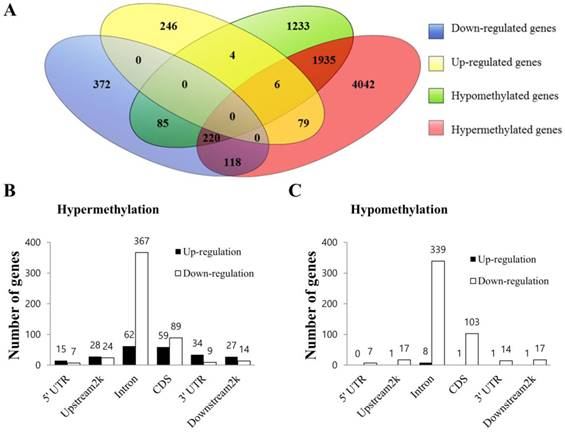
\includegraphics[width=0.8\textwidth]{journal-of-cancer_sample-result}}
%	\caption{یک نمونه نمودار خلاصه برای نمایش نوآوری در نتایج
%		%\cite{kim2016integrated}
%	}
%	\label{fig:sampleDiagram}
%\end{figure}\\
%طبیعتاً به صلاحدید نگارنده، شکل‌ها و نمودار‌ها می توانند در بخش های مختلف، خصوصا فصل
%\ref{chap:results}
%مورد استفاده قرار گیرند.
%
%\subsection{تعریف واژه‌ها (اختیاری)}
%در این قسمت محقق باید واژه‌هایی را که ممکن است برای خواننده آشنا نباشد، تعریف کند.
%
%\subsection{خلاصه فصل‌ها}
%در آخرین قسمتِ فصل اول پایان‌نامه، خلاصه‌ای اشاره‌وار از فصل‌های آتی آورده می‌شود تا خواننده بتواند تصویری واضح از دیگر قسمت‌های پایان‌نامه در ذهن خود ترسیم کند.
%
%\section{جمع‌بندی}
%در این فصل به دو مقولهٔ نحوه استفاده از قالب \پ دانشگاه تهران و نیز ویژگی‌هایی که محتویات فصل اول پایان‌نامه (یعنی مقدمه) باید داشته باشند، پرداخته شد. با توجه به اینکه این راهنما نحوه استفاده از قالب را شرح داده، ملزومات محتوایی هر فصل پایان‌نامه را توضیح می‌دهد و در پیوست‌ها نیز نحوهٔ کار با لاتک را یادآوری خواهد کرد، بنابراین مطالعهٔ کامل آن مقداری وقت شما را خواهد گرفت؛ اما مطمئن باشید از اتلاف وقت شما در ادامه کارتان تا حد زیادی جلوگیری خواهد کرد. در نوشتن متن حاضر سعی شده است علاوه بر ایجاد یک قالب لاتک برای پایان‌نامه‌های دانشگاه تهران، نکات محتوایی هر فصل نیز گوشزد گردد. طبیعتاً برای نگارش پایان‌نامهٔ خود می‌بایست مطالب تمام فصل‌ها را خودتان بازنویسی کنید.
%
%در ادامهٔ این راهنما، تنها فصل‌هایی که یک پایان‌نامه باید داشته باشد و نیز خصوصیات یا ساختاری که محتویات هر فصل باید از آنها برخوردار باشد%
%\footnote{از روی فایل «تمپلیت نگارش و تدوین پایان‌نامه \cite{UTThesisGuide}»}،
%آورده می‌شوند. نهایتاً  در پیوست‌ها، مطالبی در باب یادآوری دستورات لاتک، نحوه نوشتن فرمول‌ها، تعاریف، قضایا، مثال‌ها، درج تصاویر، نمودارها، جداول و الگوریتم‌ها و نیز مدیریت مراجع، آمده است.
%
%همچنین توصیه اکید دارم که رفع خطاهایی که احتمالاً با آنها مواجه می‌شوید را به آخر موکول نفرمایید و به محض برخورد با خطا، آن را اشکال‌زدایی و برطرف نمائید.!
%و
%\verb!% !TeX root=../main.tex
\chapter{پیشینه پژوهش}
%\thispagestyle{empty} 
\section{تولید آزمایه به صورت خودکار}
تولید خودکار آزمایه 
\LTRfootnote{Testcase}
به معنای ایجاد سناریوهای آزمون به صورت خودکار، بدون نیاز به دخالت دستی است. در این روش آزمونگر از تکنیک‌ها و ابزارهای ویژه‌ای استفاده می‌کند تا سناریوهای متنوعی برای آزمون نرم‌افزار تحت آزمون
\LTRfootnote{System Under Test}
 ایجاد کند. مزایای این روش عبارت‌اند از:
\begin{itemize}
	\item \textbf{پوشش گسترده‌تر آزمون:} تولید خودکار آزمایه‌ها، مواردی را پوشش می‌دهد که ممکن است در آزمون‌های دستی نادیده گرفته شوند. این امر به ویژه در آزمون نرم‌افزارهای پیچیده و بزرگ اهمیت بیشتری دارد.
	\item \textbf{افزایش کارایی آزمون:} با خودکارسازی فرآیند تولید آزمایه‌ها، می‌توان تعداد زیادی آزمایه در مدت زمان کوتاهی ایجاد کرد، که این کارایی در فازهای توسعه و نگهداری نرم‌افزار بسیار مفید است.
	\item \textbf{کشف باگ‌های ناشناخته:} تولید خودکار آزمایه‌ها به شناسایی باگ‌هایی کمک می‌کند که ممکن است در سناریوهای پیش‌بینی‌نشده رخ دهند. آزمون‌های تصادفی به خصوص در این زمینه بسیار مؤثر هستند.
	\item \textbf{کاهش دخالت انسانی:} خودکارسازی تولید آزمایه‌ها باعث کاهش خطاهای انسانی می‌شود و دقت و اطمینان آزمون‌ها را افزایش می‌دهد.
\end{itemize}

\section{آزمون تصادفی}
آزمون تصادفی \LTRfootnote{Random Testing} یک روش آزمون نرم‌افزار جعبه سیاه\LTRfootnote{Black Box Testing} است که در آن سیستم تحت آزمون با ورودی‌های تولید شده به صورت تصادفی ارزیابی می‌شود. هدف اصلی آزمون تصادفی، شناسایی اشکالات نرم‌افزار و اطمینان از قابلیت اطمینان و استحکام نرم‌افزار در مواجهه با انواع مختلف سناریوهای ورودی است.
\subsection{فرآیند تولید آزمایه توسط آزمون تصادفی}
فرآیند تولید آزمایه به صورت خودکار توسط روش آزمون تصادفی را می‌توان به صورت زیر ترسیم کرد:

\begin{enumerate}
	\item \textbf{تعریف فضای ورودی\LTRfootnote{Input Domain}:} در این مرحله محدوده و نوع ورودی‌هایی که نرم‌افزار می‌تواند بپذیرد، مشخص می‌گردد. این شامل تعیین دامنه‌های ورودی و محدودیت‌ها برای اطمینان از صحت موارد آزمون تولید شده است.
	\item \textbf{تولید موارد آزمون:} مجموعه‌ای از مقادیر ورودی به صورت تصادفی در داخل فضای ورودی تعریف شده تولید می‌شود. این ورودی‌ها باید طیف گسترده‌ای از سناریوهای ممکن را پوشش دهند تا احتمال کشف اشکالات افزایش یابد.
	\item \textbf{اجرای آزمون:} نرم‌افزار با استفاده از ورودی‌های تولید شده تصادفی اجرا شده و رفتار و خروجی‌های آن برای هر گونه ناهنجاری یا نتایج غیرمنتظره نظارت می‌شود.
	\item \textbf{ارزیابی خروجی‌ها:} خروجی‌های واقعی نرم‌افزار با خروجی‌های مورد انتظار (در صورت موجود بودن) مقایسه می‌شوند تا هر گونه تفاوت شناسایی گردد. در مواردی که خروجی مورد انتظار از پیش تعیین نشده است، از روش‌های اکتشافی یا اوراکل‌ها
		\LTRfootnote{Oracle}
	 برای ارزیابی درستی رفتار سیستم تحت آزمون استفاده می‌شود.
	\item \textbf{شناسایی و تحلیل اشکالات:} هر گونه انحراف یا خرابی که در حین آزمون شناسایی شود، تحلیل می‌گردد تا علل زیربنایی آن تشخیص داده شود.
\end{enumerate}


\subsection{مزایای آزمون تصادفی}
آزمون تصادفی چندین مزیت دارد که آن را به یک تکنیک ارزشمند در آزمون نرم‌افزار تبدیل می‌کند:
\begin{itemize}
	\item \textbf{سادگی:} این روش به سادگی قابل پیاده‌سازی است و نیازی به دانش عمیق از ساختار داخلی نرم‌افزار ندارد. موارد آزمون می‌توانند به صورت خودکار و بدون تلاش دستی، به صورت نامحدود تولید شوند.
	\item \textbf{خودکارسازی:} آزمون تصادفی می‌تواند به طور کامل خودکار شود و امکان آزمون پیوسته و بدون نیاز به نظارت انسانی را فراهم کند. این امر نیاز به دخالت انسانی را کاهش می‌دهد.
	\item \textbf{پوشش گسترده:} با تولید مجموعه‌ای متنوع از ورودی‌های تصادفی، آزمون تصادفی می‌تواند طیف گسترده‌ای از سناریوهای ورودی را پوشش دهد. این امر احتمال کشف اشکالات نادر یا غیرمنتظره‌ای که ممکن است از طریق دیگر روش‌های آزمون نرم‌افزار شناسایی نشوند را افزایش می‌دهد.
\end{itemize}

\subsection{معایب آزمون تصادفی}
با وجود مزایای آن، آزمون تصادفی چندین محدودیت دارد که می‌تواند بر اثربخشی آن تأثیر بگذارد:
\begin{itemize}
	\item \textbf{ناکارآمدی:} این روش می‌تواند از نظر زمان و منابع محاسباتی ناکارآمد باشد. بسیاری از ورودی‌های تولید شده ممکن است موارد آزمون معناداری را تحریک نکنند، که منجر به هدر رفتن تلاش‌ها و منابع استفاده شده جهت آزمون می‌شود.
	\item \textbf{تکرارپذیری:} آزمون تصادفی ممکن است موارد آزمون تکراری تولید کند که ارزش افزوده زیادی ندارند. نبود تمرکز بر نواحی بحرانی می‌تواند منجر به حجم بالای آزمون‌ها با نرخ شناسایی اشکال پایین شود.
	\item \textbf{تمرکز محدود:} آزمون تصادفی نواحی ورودی خاص یا نقاط خرابی بحرانی را اولویت‌بندی نمی‌کند. بنابراین، ممکن است اشکالات مهمی که در نواحی کمتر آزمون شده متمرکز شده‌اند را نادیده بگیرد.
\end{itemize}

%===============================================================================================================

\section{آزمون تصادفی تطبیقی}
آزمون تصادفی تطبیقی \LTRfootnote{Adaptive Random Testing}  با هدف بهبود آزمون تصادفی سنتی به وجود آمد و به ناکارآمدی‌ها و محدودیت‌های آن پرداخت. مفهوم آزمون تصادفی تطبیقی برای افزایش قابلیت‌های شناسایی اشکال آزمون تصادفی، با استفاده از استراتژی‌های تطبیقی که انتخاب موارد آزمون را هدایت می‌کنند، معرفی شد. آزمون تصادفی تطبیقی هدف دارد تا نرخ شناسایی اشکال بهتر را با حفظ مزایای سادگی و خودکارسازی آزمون تصادفی، بیشتر کند.

\subsection{فرضیه اصلی آزمون تصادفی تطبیقی}

توسعه آزمون تصادفی تطبیقی به دلیل نیاز به کاهش تکرارپذیری و ناکارآمدی مرتبط با تولید موارد آزمون به صورت تصادفی خالص به وجود آمد. محققان مشاهده کردند که اشکالات نرم‌افزار تمایل دارند در برخی نواحی فضای ورودی متمرکز شوند و به عبارت دیگر \textbf{نقاط خطا و شکست درون دامنه ورودی به صورت ناحیه‌ای هستند و تمایل به پیوسته بودن دارند.} در نتیجه هر چه تراکم آزمایه‌ها روی دامنه ورودی بیشتر باشد، احتمال کشف خطای جدید بیشتر خواهد بود. آزمون تصادفی تطبیقی از این مشاهده بهره می‌برد و از بازخورد موارد آزمون قبلی برای هدایت تولید موارد آزمون بعدی استفاده می‌کند. به طور کلی، آزمون تصادفی تطبیقی، آزمون تصادفی سنتی را با استفاده از تکنیک‌هایی که توزیع یکنواخت‌تری از موارد آزمون را در سراسر فضای ورودی تضمین می‌کنند، تقویت می‌کند. اصل کلیدی روش آزمون تصادفی تطبیقی این است که حداکثر تنوع موارد آزمون را به دست آورد و به این ترتیب، احتمال شناسایی خطا را افزایش دهد.

\subsection{فرآیند تولید آزمایه توسط آزمون تصادفی تطبیقی}

فرآیند تولید آزمایه به صورت خودکار توسط روش آزمون تصادفی تطبیقی را می‌توان به صورت زیر ترسیم کرد:
\begin{itemize}
	\item \textbf{تولید مجموعه کاندید\LTRfootnote{Candidate Set}:} در این مرحله ابتدایی، یک مجموعه‌ای از آزمایه‌ها با استفاده از روش آزمون تصادفی تولید می‌شود. این آزمایه‌ها به صورت تصادفی روی فضای ورودی تعریف شده از نرم‌افزار ایجاد می‌شوند.
	\item \textbf{انتخاب آزمایه:} از مجموعه کاندید تولید شده، یک آزمایه بر اساس یک استراتژی خاص که منحصراً به روش آزمون تصادفی تطبیقی مربوط است، انتخاب می‌شود. این استراتژی معمولاً به منظور به حداکثر رساندن فاصله آزمایه‌ها در فضای ورودی عمل می‌کند. با انتخاب آزمایه‌هایی که به طور گسترده‌تری پراکنده شده‌اند، آزمون تصادفی تطبیقی سعی دارد که احتمال کشف خطاها را نسبت به آزمون تصادفی سنتی افزایش دهد.
	\item \textbf{تکرار:} آزمایه انتخاب شده به مجموعه آزمایه‌های انتخاب شده \LTRfootnote{Executed Set}اضافه می‌شود و مراحل فوق به صورت تکراری انجام می‌شود. فرآیند تولید یک مجموعه کاندید جدید و انتخاب یک آزمایه ادامه می‌یابد تا زمانی که شرط خاتمه ارضاء شود که برای مثال شرط خاتمه می‌تواند رسیدن به تعداد مشخصی آزمایه باشد.
\end{itemize}
با دنبال کردن این مراحل، آزمون تصادفی تطبیقی تلاش می‌کند تا با تمرکز بر توزیع یکنواخت‌تر آزمایه‌ها، قابلیت کشف خطا را در مقایسه با آزمون تصادفی سنتی بهبود بخشد.

\subsection{مزایای آزمون تصادفی تطبیقی}
آزمون تصادفی تطبیقی چندین مزیت دارد که آن را به جایگزینی برتر برای آزمون تصادفی سنتی تبدیل می‌کند. در ادامه به برخی از این مزیت‌ها اشاره شده است:
\begin{itemize}
	\item \textbf{کاهش تکرارپذیری:} آزمون تصادفی تطبیقی با تولید موارد آزمون متنوع تکرارپذیری را کاهش می‌دهد. این امر ارزش هر مورد آزمون را به حداکثر می‌رساند و تلاش‌های بیهوده آزمون را به حداقل می‌رساند.
	\item \textbf{افزایش کارایی و نرخ شناسایی اشکال بالاتر:}‌ به دنبال کاهش تکرارپذیری موارد آزمون، کارایی روش آزمون تصادفی تطبیقی افزایش می‌یابد و فرآیند آزمون را بهبود می‌بخشد، که این خود منجر به نرخ شناسایی اشکال بالاتر با تعداد آزمایه کمتر می‌شود.
	\item \textbf{پوشش متعادل:} روش آزمون تصادفی تطبیقی، پوشش متعادل‌تری از فضای ورودی را به دست می‌آورد و خطر نادیده گرفتن نواحی مهم را کاهش می‌دهد. این پوشش جامع، استحکام کلی نرم‌افزار را افزایش می‌دهد.
	\item \textbf{بهینه‌سازی منابع:} با بهبود کارایی تولید موارد آزمون، آزمون تصادفی تطبیقی از منابع محاسباتی و زمانی بهینه استفاده می‌کند. این امر آزمون تصادفی تطبیقی را به یک راه‌حل عملی و مقیاس‌پذیر برای آزمون نرم‌افزار در مقیاس بزرگ تبدیل می‌کند.
\end{itemize}

\subsection{سربار محاسباتی پیاده سازی آزمون تصادفی تطبیقی}
در مرحله انتخاب آزمایه از فرآیند پیاده‌سازی روش آزمون تصادفی تطبیقی، لازم است که فاصله بین هر آزمایه درون مجموعه کاندید و هر آزمایه درون مجموعه آزمایه‌های انتخاب‌شده در مراحل قبلی محاسبه شود. آزمایه‌ای که بیشترین فاصله را با مجموعه آزمایه‌های انتخاب‌شده دارد، انتخاب می‌شود. در این مرحله، تعداد محاسبات فاصله باید به اندازه‌ی (تعداد آزمایه‌های درون مجموعه کاندید × تعداد آزمایه‌های درون مجموعه آزمایه‌های انتخاب‌شده) انجام شود. با افزایش تعداد اعضای مجموعه آزمایه‌های انتخاب‌شده در هر بار تکرار فرآیند، سربار محاسباتی الگوریتم آزمون تصادفی تطبیقی افزایش می‌یابد. همچنین، تعداد اعضای درون مجموعه کاندید نیز تأثیر مستقیمی بر افزایش سربار محاسباتی الگوریتم دارد. در ادامه، استراتژی‌هایی که تاکنون برای کاهش اندازه مجموعه کاندید، کاهش تعداد آزمایه‌های درون مجموعه آزمایه‌های انتخاب‌شده در مراحل قبلی الگوریتم، و در نهایت کاهش تعداد محاسبات فاصله ارائه شده‌اند، شرح داده می‌شود.

\subsubsection{اندازه مجموعه کاندید ثابت}
اولین و پرکاربردترین استراتژی پیاده‌سازی الگوریتم آزمون تصادفی تطبیقی، استراتژی "انتخاب آزمایه از مجموعه کاندید با اندازه ثابت\LTRfootnote{Fixed Sized Candidate Set (FSCS)}" است. در این استراتژی، که توسط [نام پژوهشگر/منبع] ارائه شده است، اندازه مجموعه کاندید در کل روند اجرای الگوریتم ثابت در نظر گرفته می‌شود. بهترین مقدار برای اندازه مجموعه کاندید طبق پژوهش [نام پژوهشگر/منبع] برابر با ۱۰ اعلام شده است. البته، هر چه اندازه مجموعه کاندید را افزایش دهیم، این امر می‌تواند بر اثربخشی آزمایه‌های نهایی تأثیر داشته باشد. اما بر اساس این پژوهش، هنگامی که اندازه مجموعه کاندید از ۱۰ بیشتر باشد، میزان افزایش اثربخشی مجموعه آزمایه‌ها خیلی قابل توجه نیست.

\subsubsection{بزرگ شدن فضای آزمون در آزمون تصادفی تطبیقی}
یکی از چالش‌های اصلی و مهم در آزمون تصادفی تطبیقی، بزرگ شدن فضای آزمون است. با افزایش تعداد آزمایه‌های انتخاب شده، محاسبه فاصله هر آزمایه جدید با آزمایه‌های قبلی زمان‌بر و ناکارآمد می‌شود. این مسئله باعث افزایش پیچیدگی محاسباتی و کاهش کارایی فرآیند آزمون می‌شود. برای مقابله با این مشکل، استراتژی‌های مختلفی ارائه شده‌اند که هدف آن‌ها کاهش فضای آزمون و بهبود کارایی تولید آزمایه‌ها است.
\begin{itemize}
	\item \textbf{استراتژی فراموشی\LTRfootnote{Forgetting Strategy}:} استراتژی فراموشی به منظور مدیریت فضای آزمون و جلوگیری از بزرگ شدن بیش از حد آن استفاده می‌شود. در این روش، زمانی که مجموعه آزمایه‌های از قبل انتخاب‌شده به توزیع یکنواخت مناسبی می‌رسند، این مجموعه پاک می‌شود. با این کار، فقط آزمایه‌های جدیدتر و مرتبط‌تر در فرآیند محاسبه فاصله‌ها لحاظ می‌شوند. در این استراتژی با پاک کردن آزمایه‌های قدیمی‌تر، حجم داده‌های مورد نیاز برای محاسبه فاصله‌ها کاهش می‌یابد و محاسبات سریع‌تر و کارآمدتر انجام می‌شود. البته، احتمال از دست رفتن اطلاعات مفید از آزمایه‌های قبلی وجود دارد و همچنین معیارهای فراموشی باید به دقت تنظیم شوند تا بهترین نتیجه حاصل شود.
	
	\item \textbf{خوشه‌بندی \lr{K}-مرکز\LTRfootnote{K-means Clustering Strategy}:} خوشه‌بندی \lr{K}-مرکز یکی دیگر از استراتژی‌های کاهش فضای آزمون است. در این روش، آزمایه‌های انتخاب‌شده به خوشه‌هایی تقسیم می‌شوند و هر خوشه با یک نماینده (میانگین) که مرکز خوشه است، مشخص می‌شود. برای انتخاب آزمایه جدید، فاصله بین آزمایه‌های کاندید و نمایندگان خوشه‌ها محاسبه می‌شود. این استراتژی علاوه بر کاهش تعداد محاسبات فاصله، باعث مدیریت بهتر فضای آزمون می‌شود و فضای آزمون به صورت خوشه‌بندی‌شده نگهداری می‌شود. با این حال، این روش ممکن است پیچیدگی اجرای الگوریتم را افزایش دهد و تعیین تعداد خوشه‌ها (\lr{K}) باید به دقت انجام شود تا بهترین نتیجه حاصل شود.
	
	\item \textbf{استراتژی شبکه‌بندی\LTRfootnote{Grid Strategy}:} در این روش، فضای ورودی به سلول‌های کوچکتری تقسیم می‌شود. آزمایه‌های انتخاب‌شده در هر سلول ذخیره می‌شوند و برای انتخاب آزمایه جدید، فقط سلول‌های مجاور مورد بررسی قرار می‌گیرند. این استراتژی علاوه بر کاهش تعداد محاسبات فاصله، باعث مدیریت بهتر فضای آزمون می‌شود و فضای آزمون به صورت شبکه‌بندی‌شده نگهداری می‌شود. با این حال، این روش به پیاده‌سازی دقیق شبکه‌بندی نیاز دارد و اندازه سلول‌ها باید به دقت تنظیم شود تا بهترین نتیجه حاصل شود.

\end{itemize}

\subsection{اولین پیاده‌سازی روش آزمون تصادفی تطبیقی}
اولین پیاده‌سازی روش آزمون تصادفی تطبیقی روی برنامه‌هایی با ورودی عددی\LTRfootnote{Numerical Input Domain} انجام شد. در این پیاده‌سازی، هر آزمایه که مجموعه‌ای از ورودی‌های عددی بود، به صورت یک نقطه درون یک فضای چندبعدی (تعداد ابعاد برابر با تعداد ورودی‌ها) مدل‌سازی شد. در ادامه، این الگوریتم روی یک مثال ساده بررسی می‌شود.

فرض کنید که یک برنامه به نام \lr{Sum} دارید که دو عدد به عنوان ورودی دریافت کرده و حاصل جمع آن‌ها را برمی‌گرداند. در این الگوریتم، آزمایه‌های این برنامه روی یک فضای دوبعدی به صورت نقطه مدل خواهند شد (برای مثال، آزمایه با ورودی‌های ۱۰ و ۱۵ در فضای ورودی دوبعدی نقطه \lr{(10,15)} را تشکیل می‌دهد) و فاصله بین آن‌ها، همان فاصله اقلیدسی\LTRfootnote{Euclidean distance} بین دو نقطه در نظر گرفته می‌شود.

این روش با روش آزمون تصادفی سنتی روی چند برنامه مختلف با ورودی عددی پیاده‌سازی شد و نتایج نشان داد که این روش از روش آزمون تصادفی سنتی کارایی و عملکرد بهتری دارد.

اما مهم‌ترین مشکل این روش این بود که تنها روی برنامه‌هایی با ورودی عددی قابل پیاده‌سازی بود. با این حال، این مسئله باعث شد که زمینه پژوهشی جدیدی برای محققان ایجاد شود تا راهکاری برای محاسبه فاصله بین دو آزمایه با ورودی‌های غیرعددی\LTRfootnote{Obejctive} ارائه دهند. در اکثر راهکارهای ارائه‌شده، تلاش بر این بوده که هر آزمایه را به عنوان یک نقطه در یک یا چند فضای چندبعدی مدل کنند و سپس با استفاده از محاسبات ریاضی رایج برای محاسبه فاصله در فضاهای چندبعدی، مانند فاصله اقلیدسی، فاصله بین دو نقطه را به دست آورده و به عنوان فاصله بین دو آزمایه ارائه دهند.

\subsection{آخرین ایده پیاده‌سازی ارائه شده برای روش آزمون تصادفی تطبیقی}
آخرین روشی که تاکنون در این حوزه توسط [نام پژوهشگر/منبع] ارائه شده است، شامل روش‌های \lr{WTClustering-ART} و \lr{TFClustering-ART} می‌باشد. در ادامه به بررسی دقیق ساختار و نحوه کارکرد هر کدام از این روش‌ها پرداخته شده است.

\subsubsection{تبدیل فرکانس }
کاهوچی و همکارانش روش‌هایی بر مبنای تبدیل فرکانس\LTRfootnote{Frequency Transform}، که قبلاً برای تبدیل رشته‌ها در جستجوی تشابه رشته‌ها استفاده می‌شد، پیشنهاد کردند. این روش یک رشته با طول تعریف‌شده را با تعداد دفعات هر کاراکتر در رشته به یک بردار فرکانس\LTRfootnote{Frequency Vector} تبدیل می‌کند. تعریف دقیق بردار فرکانس در ادامه آورده شده است.

\begin{itemize}
	\item \textbf{بردار فرکانس:}
	فرض کنید که \(\Sigma = \{m_1, m_2, \dots, m_n\}\) لیست توابع در یک برنامه فرضی باشد و \(s\) ترتیب فراخوانی توابع توسط آزمایه \(t\) باشد. حال بردار فرکانس به صورت 
	\(f(s) = \{f_1, f_2, \dots, f_n\}\)
	 تعریف خواهد شد که \(f_i\) تعداد دفعاتی است که تابع \(m_i\) در ترتیب فراخوانی توابع (\(s\)) حضور دارد.
	
	برای مثال فرض کنید که \(\Sigma = \{a, b, c, d, e\}\) و \(s = abddc\) ترتیب فراخوانی توابع در حین اجرای آزمایه \(t\) باشد. در این وضعیت، تابع \(a\) یک بار، \(b\) یک بار، \(c\) صفر بار، \(d\) دو بار و \(e\) یک بار فراخوانی شده است. در نتیجه:
	\[
	f(s) = \{1, 1, 0, 2, 1\}
	\]
	
	حال با توجه به اینکه هر آزمایه به یک لیست عددی با طول \(n\) (یک نقطه در فضای \(n\) بعدی) تبدیل شده است، اکنون می‌توان به سادگی فاصله بین آزمایه‌ها را با استفاده از محاسبه فاصله بین نقطه‌های متناظر آزمایه‌ها به دست آورد.
	
\end{itemize}

\subsubsection{تبدیل موجک}
اگرچه تبدیل فرکانس می‌تواند به راحتی آزمایه‌های شیء‌گرا را به بردارهایی برای اندازه‌گیری عدم تشابه تبدیل کند، اما فقط بر فرکانس فراخوانی توابع تمرکز می‌کند و به ترتیب فراخوانی توابع اهمیتی نمی‌دهد. از آنجایی که ترتیب واقعی فراخوانی توابع معمولاً بر نتایج اجرا تأثیر می‌گذارد، عدم تشابه محاسبه‌شده رضایت‌بخش نیست.

برای مثال، فرض کنید \(\Sigma = \{a, b, c, d, e\}\) و \(s_1 = acbe\) ترتیب فراخوانی توابع در آزمایه \(t_1\) و \(s_2 = bcae\) ترتیب فراخوانی توابع در آزمایه \(t_2\) باشد. بعد از انجام تبدیل فرکانس، دو بردار فرکانس\\ \(f(s_1) = f(s_2) = \{1, 1, 1, 0, 1\}\) به دست خواهد آمد. فاصله بین آزمایه \(t_1\) و \(t_2\) با توجه به مقایسه بردارهای فرکانس این دو آزمایه صفر است، در حالی که ترتیب فراخوانی توابع در دو آزمایه کاملاً یکسان نیست.

از این رو، روش تبدیل موجک در این مقاله ارائه شد که علاوه بر تعداد فراخوانی هر تابع، به ترتیب فراخوانی توابع نیز تا حدی اهمیت می‌دهد. تبدیل موجک\LTRfootnote{Wavelet Transform} ابزاری ریاضی است که برای تجزیه و تحلیل سیگنال‌ها و داده‌ها در حوزه زمان و فرکانس استفاده می‌شود. در این مقاله، از تبدیل موجک برای اندازه‌گیری عدم تشابه بین تست‌ کیس‌های شیءگرا استفاده می‌شود. این معیار با تجزیه و تحلیل سیگنال‌های مربوط به ویژگی‌های آزمایه‌ها، میزان تفاوت بین آن‌ها را محاسبه می‌کند. در روش
 \lr{ART\_WTClustering} 
 از موجک هار \LTRfootnote{Haar Wavelet} برای مدل‌سازی اطلاعات فرکانس و اطلاعات ترتیب فراخوانی توابع استفاده شده است. در ادامه، معیار تبدیل موجک با مثال توضیح داده شده است.

\begin{itemize}
	\item \textbf{تعریف تبدیل موجک آزمایه:}
فرض کنید \(s = m_1 m_2 \dots m_j\) ترتیب فراخوانی توابع باشد. \(s_1\) یک زیررشته از \(s\) است که حاوی نیمه اول عناصر \(s\) است و \(s_2\) یک زیررشته دیگر از \(s\) است که حاوی نیمه دوم عناصر \(s\) است. تبدیل موجک \(s\) به صورت \(W(s) = [A, B]\) تعریف می‌شود که \(A = f(s)\) و \(B = B_1 - B_2\) که \(B_1 = f(s_1)\) و \(B_2 = f(s_2)\) است.

برای مثال فرض کنید که \(\Sigma = \{a, b, c, d, e\}\) و \(s = abdde\) ترتیب فراخوانی توابع در حین اجرای آزمایه \(t\) باشد. حال مقادیر \(A\) , \(B\) و \(W(s)\) به صورت زیر محاسبه خواهند شد:
\begin{align*}
	A = f(s) &= \{1, 1, 0, 2, 1\} \\
	s_1 = ab \quad & \Rightarrow \quad B_1 = \{1, 1, 0, 0, 0\} \\
	s_2 = dde \quad &\Rightarrow \quad B_2 = \{0, 0, 0, 2, 1\} \\
	B = B_1 - B_2 \quad &\Rightarrow \quad B = \{1, 1, 0, -2, -1\} \\
	W(s) = [A, B] \quad &\Rightarrow \quad W(s) = \left[\{1, 1, 0, 2, 1\}, \{1, 1, 0, -2, -1\}\right]
\end{align*}

\item \textbf{محاسبه فاصله بین آزمایه‌‌ها:}
فرض کنید \(\Sigma = \{m_1, m_2, \dots, m_n\}\) لیست توابع درون یک برنامه فرضی باشد. اگر \(s_1\) ترتیب فراخوانی توابع توسط آزمایه \(t_1\) و \(s_2\) ترتیب فراخوانی توابع توسط آزمایه \(t_2\) باشد، آنگاه \(W(s_1) = [A_1, B_1]\) و \(W(s_2) = [A_2, B_2]\) خواهد بود که \(A_1 = \{A_{11}, A_{12}, \dots, A_{1n}\}\) و \(B_1 = \{B_{11}, B_{12}, \dots, B_{1n}\}\) و \(A_2 = \{A_{21}, A_{22}, \dots, A_{2n}\}\) و \(B_2 = \{B_{21}, B_{22}, \dots, B_{2n}\}\) که فاصله \(WT\_D\) بین این دو آزمایه به صورت زیر محاسبه خواهد شد:
\[
WT\_D(t_1, t_2) = \sqrt{\sum_{i=1}^{n} (A_{1i} - A_{2i})^2} + \sqrt{\sum_{i=1}^{n} (B_{1i} - B_{2i})^2}
\]


\end{itemize}

\subsubsection{تبدیل فرکانس سه‌بخشی}
تا حدی، استفاده مستقیم از تبدیل موجک برای آزمایه‌های شیءگرا نامناسب است. دلیل اصلی این است که، اگرچه دنباله فراخوانی توابع را به دو قسمت تقسیم می‌کند و آنها را حفظ می‌کند، اما تنها تفریق نیمه اول و دوم این دنباله نمی‌تواند تفاوت بین توالی فراخوانی توابع را نمایش دهد. برای پرداختن به این موضوع، در این مقاله پیشنهاد شده است که از تبدیل فرکانس سه‌بخشی \LTRfootnote{Trisection Frequency Conversion (TFC)} استفاده شود. این معیار نه تنها به تعداد فراخوانی هر تابع در حین اجرای آزمایه‌ها توجه دارد بلکه ترتیب فراخوانی توابع در حین اجرای آزمایه‌های مختلف نیز اهمیت دارد.

\begin{itemize}

\item \textbf{تعریف معیار تبدیل فرکانس سه‌بخشی:}
فرض کنید که \(s = m_1 m_2 \dots m_j\) ترتیب فراخوانی توابع در حین اجرای آزمایه \(t\) باشد و \(s_1\) نیمه اول \(s\) و \(s_2\) نیمه دوم \(s\) باشد. معیار تبدیل فرکانس سه‌بخشی برای \(s\) به صورت \(TF(s) = [A, B, C]\) نمایش داده می‌شود که \(A = f(s)\)، \(B = f(s_1)\) و \(C = f(s_2)\) است.

\item \textbf{محاسبه فاصله بین آزمایه‌‌ها:}

فرض کنید \(\Sigma = \{m_1, m_2, \dots, m_n\}\) لیست توابع در یک برنامه فرضی باشد. یک آزمایه \(t_1\) با دنباله فراخوانی توابع \(s_1\) و یک آزمایه \(t_2\) با دنباله فراخوانی توابع \(s_2\) را در نظر بگیرید. فرض کنید\\ \(TF(s_1) = [A_1, B_1, C_1]\) و \(TF(s_2) = [A_2, B_2, C_2]\) که در آن \(A_1 = \{A_{11}, A_{12}, \dots, A_{1n}\}\)، \(B_1 = \{B_{11}, B_{12}, \dots, B_{1n}\}\)، \(C_1 = \{C_{11}, C_{12}, \dots, C_{1n}\}\)، \(A_2 = \{A_{21}, A_{22}, \dots, A_{2n}\}\)، \(B_2 = \{B_{21}, B_{22}, \dots, B_{2n}\}\)، و \(C_2 = \{C_{21}, C_{22}, \dots, C_{2n}\}\). تفاوت ترتیب بین \(s_1\) و \(s_2\) به صورت \(\sum_{i=1}^{j} \left(1 - \delta_{s_{1i} s_{2i}}\right)\) تعریف می‌شود، که \(\delta_{s_{1i} s_{2i}}\) نماد دلتای کرونکر استاندارد است، به طوری که اگر \(s_{1i} = s_{2i}\) باشد آنگاه \(\delta_{s_{1i} s_{2i}} = 1\) و در غیر اینصورت \(\delta_{s_{1i} s_{2i}} = 0\). فاصله \(TFC\)  یا \(TFC\_D\) بین این دو آزمایه به صورت زیر تعریف می‌شود:

\[
TFC\_D(t_1, t_2) = \sqrt{\sum_{i=1}^{n} (A_{1i} - A_{2i})^2} + \sqrt{\sum_{i=1}^{n} (B_{1i} - B_{2i})^2}
\]
\[
+ \sqrt{\sum_{i=1}^{n} (C_{1i} - C_{2i})^2} + \sum_{i=1}^{n} \left(1 - \delta_{s_{1i} s_{2i}}\right)
\quad
\]

\end{itemize}

\subsubsection{مقایسه بین \(TFC\_D\) و \(WT\_D\):}
در اینجا به بررسی تفاوت‌های \(WT\_D\) و \(TFC\_D\) در یک مثال پرداخته شده است. دو آزمایه \(t_1\) و \(t_2\) را در نظر بگیرید که ترتیب فراخوانی توابع توسط این دو آزمایه به صورت \(s_1 = abce\) و \(s_2 = abec\) است که \(s_{11} = ab\)، \(s_{12} = ce\)، \(s_{21} = ab\) و \(s_{22} = ec\) است. در نتیجه:

\begin{align*}
	W(s_1) &= \left[\langle 1, 1, 1, 0, 1 \rangle, \langle 1, 1, -1, 0, -1 \rangle \right] \\
	W(s_2) &= \left[\langle 1, 1, 1, 0, 1 \rangle, \langle 1, 1, -1, 0, -1 \rangle \right]
\end{align*}

است و در نتیجه \({WT\_D}(s_1, s_2)\) برابر است با:

\[
WT\_D(s_1, s_2) = \sqrt{0^2 + 0^2 + 0^2 + 0^2 + 0^2} + \sqrt{0^2 + 0^2 + 0^2 + 0^2 + 0^2} = 0
\]
\textbf{}
از طرفی با توجه به تعریف \(TF(s_i)\) مقادیر \(TF(s_1)\) و \(TF(s_2)\) و \(TFC\_D(s_1, s_2)\) به صورت زیر محاسبه می‌شوند:
\[
TF(s_1) = \left[\langle 1, 1, 1, 0, 1 \rangle, \langle 1, 1, 0, 0, 0 \rangle, \langle 0, 0, 1, 0, 1 \rangle\right]
\]
\[
TF(s_2) = \left[\langle 1, 1, 1, 0, 1 \rangle, \langle 1, 1, 0, 0, 0 \rangle, \langle 0, 0, 1, 0, 1 \rangle\right]
\]

\(TFC\_D(s_1, s_2)\) به صورت زیر محاسبه می‌شود:

\begin{align*}
	TFC\_D(s_1, s_2) &= \sqrt{0^2 + 0^2 + 0^2 + 0^2 + 0^2} + \sqrt{0^2 + 0^2 + 0^2 + 0^2 + 0^2} \\
	&\quad + \sqrt{0^2 + 0^2 + 0^2 + 0^2 + 0^2} + \sum_{i=1}^{j} \left(1 - \delta_{s_{1i}s_{2i}}\right)
\end{align*}

که

\[
\sum_{i=1}^{j} \left(1 - \delta_{s_{1i}s_{2i}}\right) = (1-1) + (1-1)  + (1-0)  + (1-0) = 2
\]

بنابراین:

\[
TFC\_D(s_1, s_2) = 0 + 0 + 0 + 2 = 2 
\]

همانطور که مشاهده کردید،‌ فاصله \(TFC\) در این مثال نسبت به فاصله \(ٌُWT\)  به ترتیب فراخوانی توابع توسط آزمایه‌ها اهمیت بیشتری می دهد.


\newpage

	\begin{tikzpicture}[node distance=2.5cm]
		
		\node (start) [startstop] {\rl{به صورت تصادفی اولین مورد آزمایشی شئ‌گرا را ایجاد کرده و اجرا کنید}};
		\node (decision) [decision, below of=start, yshift=-1cm] {\rl{شرط خاتمه}};
		\node (output) [startstop, right of=decision, xshift=4cm] {\rl{خروجی آزمایه‌های تولید شده}};
		\node (process1) [process, below of=decision, yshift=-1cm] {\rl{اضافه کردن این آزمایه به مجموعه آزمایه‌های انتخاب شده در مراحل قبلی الگوریتم}};
		\node (process2) [process, below of=process1, yshift=-1cm] {\rl{تولید ۱۰ آزمایه شئ‌گرا جدید به عنوان مجموعه کاندید}};
		
		\node (process3) [process, below of=process2, yshift=-1cm, xshift=0.5cm, text width=7cm] {\rl{خوشه‌بندی مجموعه آزمایه‌های از قبل انتخاب شده به \rl{K} خوشه}};
		\node (process4) [process, below of=process3, yshift=-0.5cm] {\rl{تعیین نماینده هر خوشه برای ارزیابی آزمایه‌های کاندید}};
		\node (process5) [process, below of=process4, yshift=-0.5cm] {Select the candidate which has the smallest distance with the subset};
		
		\draw [arrow] (start) -- (decision);
		\draw [arrow] (decision) -- node[anchor=east] {No} (process1);
		\draw [arrow] (decision) -- node[anchor=north] {Yes} (output);
		\draw [arrow] (process1) -- (process2);
		\draw [arrow] (process2) -- (process3);
		\draw [arrow] (process3) -- (process4);
		\draw [arrow] (process4) -- (process5);
%		\draw [arrow] (process5.east) -| ++(4,0) |- (decision.east);
		
		% Adding labels ①, ②, ③
%		\node[draw=none, fill=none] at ($(process2)!0.5!(process3)$) {\textcircled{1}};
%		\node[draw=none, fill=none] at ($(process3)!0.5!(process4)$) {\textcircled{2}};
%		\node[draw=none, fill=none] at ($(process4)!0.5!(process5)$) {\textcircled{3}};
		
	\end{tikzpicture}



\subsection{روش‌های مختلف انتخاب آزمایه بر اساس فاصله}


\subsection{نقطه اشتراک اکثر روش‌های پیاده‌سازی الگوریتم آزمون تصادفی تطبیقی}

\section{روش تقسیم‌بندی فضای ورودی}

\subsection{فرآیند تولید آزمایه توسط روش تقسیم‌بندی فضای ورودی}

%===============================================================================================================




%
%
%
%\newpage
%\section{مقدمه}
%هدف از این فصل که با عنوان‌های  «مروری بر ادبیات موضوع%
%\LTRfootnote{Literature Review}»،
%«مروری بر منابع» و یا «مروری بر پیشینه تحقیق%
%\LTRfootnote{Background Research}»
%معرفی می‌شود، بررسی و طبقه‌بندی یافته‌های تحقیقات دیگر محققان در سطح دنیا و تعیین و شناسایی خلأهای تحقیقاتی است. آنچه را که تحقیق شما به دانش موجود اضافه می‌کند، مشخص کنید. طرح پیشینه تحقیق%
%\LTRfootnote{Background Information}
%یک مرور محققانه است و تا آنجا باید پیش برود که پیش‌زمینهٔ تاریخی مناسبی از تحقیق را بیان کند و جایگاه تحقیق فعلی را در میان آثار پیشین نشان دهد. برای این منظور منابع مرتبط با تحقیق را بررسی کنید، البته نه آنچنان گسترده که کل پیشینه تاریخی بحث را در برگیرد. برای نوشتن این بخش:
%\begin{itemize}
%	\item
%	دانستنی‌های موجود و پیش‌زمینهٔ تاریخی و وضعیت کنونی موضوع را چنان بیان کنید که خواننده بدون مراجعه به منابع پیشین، نتایج حاصل از مطالعات قبلی را درک و ارزیابی کند.
%	\item
%	نشان دهید که بر موضوع احاطه دارید. پرسش تحقیق را همراه بحث و جدل‌ها و مسائل مطرح شده بیان کنید و مهم‌ترین تحقیق‌های انجام شده در این زمینه را معرفی نمائید.
%	\item
%	ابتدا مطالب عمومی‌تر و سپس پژوهش‌های مشابه با کار خود را معرفی کرده و نشان دهید که تحقیق شما از چه جنبه‌ای با کار دیگران تشابه یا تفاوت دارد.
%	\item
%	اگر کارهای قبلی را خلاصه کرده‌اید، از پرداختن به جزئیات غیرضروری بپرهیزید. در عوض، بر یافته‌ها و مسائل روش‌شناختی مرتبط و نتایج اصلی تأکید کنید و اگر بررسی‌ها و منابع مروری عمومی دربارهٔ موضوع موجود است، خواننده را به آنها ارجاع دهید.
%\end{itemize}
%
%\section{تعاریف، اصول و مبانی نظری}
%این قسمت ارائهٔ خلاصه‌ای از دانش کلاسیک موضوع است. این بخش الزامی نیست و بستگی به نظر استاد راهنما دارد.
%
%\section{مروری بر ادبیات موضوع}
%در این قسمت باید به کارهای مشابه دیگران در گذشته اشاره کرد و وزن بیشتر این قسمت بهتر است به مقالات ژورنالی سال‌های اخیر (۲ تا ۳ سال) تخصیص داده شود. به نتایج کارهای دیگران با ذکر دقیق مراجع باید اشاره شده و جایگاه و تفاوت تحقیق شما نیز با کارهای دیگران مشخص شود. استفاده از مقالات ژورنال‌های معتبر در دو یا سه سال اخیر، می‌تواند به اعتبار کار شما بیافزاید.
%
%\section{نتیجه‌گیری}
%‌در نتیجه‌گیری آخر این فصل، با توجه به بررسی انجام شده بر روی مراجع تحقیق، بخش‌های قابل گسترش و تحقیق در آن حیطه و چشم‌اندازهای تحقیق مورد بررسی قرار می‌گیرند.	در برخی از تحقیقات، نتیجه نهایی فصل روش تحقیق، ارائهٔ یک چارچوب کار تحقیقی 
%\lr{(research framework)}
است.!
%را در فایل 
%\lr{main.tex}،
%غیرفعال%
%\footnote{
%برای غیرفعال کردن یک دستور، کافی است در ابتدای آن، علامت درصد انگلیسی (\%) بگذارید.
%}
% کنید. در غیر این صورت، ابتدا مطالب دو فصل اول پردازش شده و سپس مطالب فصل ۳ پردازش می‌شود که این کار باعث طولانی شدن زمان پردازش می‌گردد. هر زمان که خروجی کل \پ را خواستید، تمام فصل‌ها را دوباره در
%\lr{main.tex}
%فعال نمائید.
%بدیهتاً لازم نیست فصل‌های \پ را به ترتیب تایپ کنید. مثلاً می‌توانید ابتدا مطالب فصل ۳ را تایپ نموده و سپس مطالب فصل ۱ را تایپ کنید. 
%\subsubsection{مراجع}
%برای وارد کردن مراجع \پ کافی است فایل 
%\lr{MyReferences.bib}
%را باز کرده و مراجع خود را به شکل اقلام نمونهٔ داخل آن، وارد کنید.  سپس از \lr{bibtex} برای تولید مراجع با قالب مناسب استفاده نمائید. برای توضیحات بیشتر بخش \ref{Sec:Ref} از پیوست \ref{app:latexIntro} و نیز پیوست \ref{app:refMan} را ببینید.
%
%\subsubsection{واژه‌نامه فارسی به انگلیسی و برعکس}
%برای وارد کردن معادل فارسی اصطلاحات لاتین در متن و تهیه فهرست واژه‌نامه از آنها، از بستهٔ
%\lr{glossaries}
%و نرم‌افزار
%\lr{xindy}
%استفاده می‌شود. بدین منظور کافی است اصطلاحات لاتین و ترجمهٔ آنها را در فایل
%\lr{words.tex}
%وارد کرده و هر جای متن که خواستید با دستورات
%\verb|gls{label}|
%یا \verb|glspl{label}|
%معادل فارسی مفرد یا جمع یک اصطلاح را بیاورید.
%
%مثلا در اینجا، واژهٔ
%«\gls{Action}»
%برای بار اول و دوباره
%«\gls{Action}»
%برای بار دوم در متن ظاهر شده است.
%جهت توضیحات بیشتر به پیوست
%\ref{app:refMan}
%مراجعه کنید.
%\subsubsection{نمایه}
%برای وارد کردن نمایه، باید از 
%\lr{xindy}
%استفاده کنید. 
%%زیرا 
%%\lr{MakeIndex}
%%با حروف «گ»، «چ»، «پ»، «ژ» و «ک» مشکل دارد و ترتیب الفبایی این حروف را رعایت نمی‌کند. همچنین، فاصله بین هر گروه از کلمات در 
%%\lr{MakeIndex}،
%%به درستی رعایت نمی‌شود که باعث زشت شدن حروف‌چینی این قسمت می‌شود. 
%راهنمای چگونگی کار با 
%\lr{xindy} 
%را می‌توانید در ویکی پارسی‌لاتک و یا مثالهای موجود در دی‌وی‌دی «مجموعه پارسی‌لاتک»، پیدا کنید.
%
%\subsection{اگر سوالی داشتم، از کی بپرسم؟}
%برای پرسیدن سوال‌های خود موقع حروف‌چینی با زی‌پرشین، می‌توانید به
%\href{http://qa.parsilatex.com}{سایت پرسش و پاسخ پارسی‌لاتک}%
%\LTRfootnote{http://qa.parsilatex.com}
%یا
%\href{http://forum.parsilatex.com}{بایگانی تالارگفتگوی قدیمی پارسی‌لاتک}%
%\LTRfootnote{http://forum.parsilatex.com}
%مراجعه کنید. شما هم می‌توانید روزی به سوال‌های دیگران در اینترنت جواب دهید.
%بستهٔ زی‌پرشین و بسیاری از بسته‌های مرتبط با آن مانند
%\lr{bidi} و
%\lr{Persian-bib}،
%مجموعه پارسی‌لاتک، مثالهای مختلف موجود در آن، قالب پایان‌نامه دانشگاههای مختلف و سایت پارسی‌لاتک همه به صورت داوطلبانه توسط افراد گروه پارسی‌لاتک و گروه
%\lr{Persian TeX}
%و بدون هیچ کمک مالی انجام شده‌اند. کار اصلی نوشتن و توسعه زی‌پرشین توسط آقای وفا خلیقی انجام شده است که این کار بزرگ را به انجام رساندند.
%اگر مایل به کمک به گروه پارسی‌لاتک هستید به سایت این گروه مراجعه فرمایید:
%\begin{center}
%	\url{http://www.parsilatex.com}
%\end{center}
%
%\section{محتویات فصل اول یک پایان‌نامه}
%فصل اول یک پایان‌نامه باید به مقدمه یا کلیات تحقیق بپردازد.
%هدف از فصل مقدمه%
%\LTRfootnote{Introduction}،
%شرح مختصر مسأله تحقیق، اهمیت و انگیزه محقق از پرداختن به آن موضوع، بهمراه اشاره‌ای کوتاه به روش و مراحل تحقیق است. مقدمه، اولین فصل از ساختار اصلی \پ بوده و زمینه اطلاعاتی لازم را برای خواننده فراهم می‌آورد. در طول مقدمه باید سعی شود موضوع تحقیق با زبانی روشن، ساده و بطور عمیق و هدفمند به خواننده معرفی شود. این فصل باید خواننده را مجذوب و اهمیت موضوع تحقیق را آشکار سازد. در مقدمه باید با ارائهٔ سوابق، شواهد تحقیقی و اطلاعات موجود (با ذکر منبع) با روشی منظم، منطقی و هدف‌دار، خواننده را جهت داد و به سوی راه حل مورد نظر هدایت کرد. مقدمه مناسب‌ترین جا برای ارائهٔ اختصارات و بعضی توضیحات کلی است، توضیحاتی که شاید نتوان در مباحث دیگر آنها را شرح داد.
%
%مقدمه، یکی از ارکان اساسی و اصلی پایان نامه است که مهمترین قسمت‌های آن عبارتند از: 
%
%\subsection{عنوان تحقیق} 
%باید شناختی دقیق و روشن از حوزهٔ موضوع تحقیق را عرضه دارد و خالی از هرگونه ابهام و پیچیدگی باشد.
%
%\subsection{مسأله تحقیق}
%وظیفه اصلی مقدمه بیان این مطلب به خواننده است که چرا انجام تحقیق را به عهده گرفته‌اید. اگر دلیل شما برای انجام این کار پاسخگویی به سؤال مورد علاقه‌تان است، با مشکل زیادی روبه‌رو نخواهید بود. یکی از بهترین روش‌ها برای نوشتن مقدمهٔ یک پایان‌نامه، طرح پرسش یا پرسش‌هایی مهم و اساسی است که کار تحقیقاتی شما از آغاز تا پایان قصد پاسخ دادن به آن را دارد. گاهی می‌توانید ابتدا اهمیت موضوع را بیان و سپس پرسش خود را در آن موضوع مطرح کنید.
%
%\subsection{تاریخچه‌ای از موضوع تحقیق}
%به طور کلی تشریح روندهای تحقیقاتی در محدودهٔ مورد مطالعه، مستلزم ارجاع به کارهای دیگران است. بعضی از نویسندگان برای کارهای دیگران هیچ اعتباری قائل نمی‌شوند و در مقابل، بعضی دیگر از نویسندگان در توصیف کارهای دیگران، بسیار زیاده‌روی می‌کنند. اکثر مواقع، ارجاع به مقالات دو سال قبل از کارتان، بهتر از نوشتن سطرهای مرجع است. در این قسمت باید به طور مختصر به نظرات و تحقیقات مربوط به موضوع و یا مسائل و مشکلات حل نشده در این حوزه و همچنین توجه و علاقه جامعه به این موضوع، اشاره شود.
%
%\subsection{تعریف موضوع تحقیق}
%در این قسمت محقق، موضوع مورد علاقه و یا نیاز احساس شدهٔ خود را در حوزه تحقیق بیان می‌دارد و عوامل موجود در موقعیت را تعریف و تعیین می‌کند.
%
%\subsection{هدف یا هدف‌های کلی و آرمانی تحقیق}
%این قسمت باید با جملات مثبت و کلی طرح شود و از طولانی شدن مطالب پرهیز شود.
%
%\subsection{روش انجام تحقیق}
%در این قسمت، پژوهشگر روش کاری خود را بیان می‌دارد و شیوه‌های گوناگونی را که در گردآوری مطالب خود بکار برده، ذکر می‌کند. همچنین اگر روش آماری خاصی را در تهیه و تدوین اطلاعات به کار برده است، آن شیوه را نیز اینجا بیان می‌کند.
%
%\subsection{نوآوری، اهمیت و ارزش تحقیق}
%در این قسمت، در مورد نوآوری علمی و عملی تحقیق که محقق به آن دست خواهد یافت، بحث می‌شود. ممکن است لازم باشد تا برخی نمودارهای خلاصه در این بخش استفاده شوند. به عنوان مثال، نموداری از مقاله
%\cite{kim2016integrated}
%در شکل
%\ref{fig:sampleDiagram}
%آمده است.
%\begin{figure}[ht]
%	\centerline{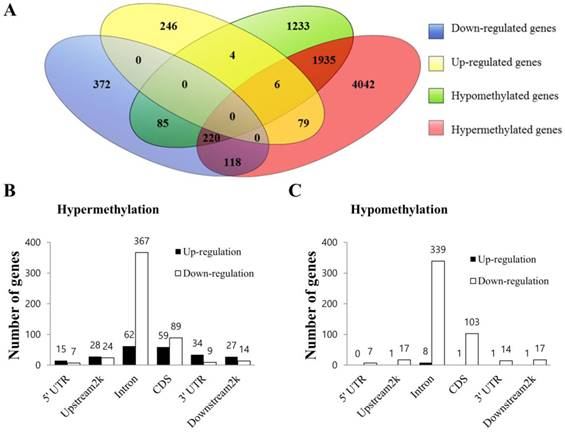
\includegraphics[width=0.8\textwidth]{journal-of-cancer_sample-result}}
%	\caption{یک نمونه نمودار خلاصه برای نمایش نوآوری در نتایج
%		%\cite{kim2016integrated}
%	}
%	\label{fig:sampleDiagram}
%\end{figure}\\
%طبیعتاً به صلاحدید نگارنده، شکل‌ها و نمودار‌ها می توانند در بخش های مختلف، خصوصا فصل
%\ref{chap:results}
%مورد استفاده قرار گیرند.
%
%\subsection{تعریف واژه‌ها (اختیاری)}
%در این قسمت محقق باید واژه‌هایی را که ممکن است برای خواننده آشنا نباشد، تعریف کند.
%
%\subsection{خلاصه فصل‌ها}
%در آخرین قسمتِ فصل اول پایان‌نامه، خلاصه‌ای اشاره‌وار از فصل‌های آتی آورده می‌شود تا خواننده بتواند تصویری واضح از دیگر قسمت‌های پایان‌نامه در ذهن خود ترسیم کند.
%
%\section{جمع‌بندی}
%در این فصل به دو مقولهٔ نحوه استفاده از قالب \پ دانشگاه تهران و نیز ویژگی‌هایی که محتویات فصل اول پایان‌نامه (یعنی مقدمه) باید داشته باشند، پرداخته شد. با توجه به اینکه این راهنما نحوه استفاده از قالب را شرح داده، ملزومات محتوایی هر فصل پایان‌نامه را توضیح می‌دهد و در پیوست‌ها نیز نحوهٔ کار با لاتک را یادآوری خواهد کرد، بنابراین مطالعهٔ کامل آن مقداری وقت شما را خواهد گرفت؛ اما مطمئن باشید از اتلاف وقت شما در ادامه کارتان تا حد زیادی جلوگیری خواهد کرد. در نوشتن متن حاضر سعی شده است علاوه بر ایجاد یک قالب لاتک برای پایان‌نامه‌های دانشگاه تهران، نکات محتوایی هر فصل نیز گوشزد گردد. طبیعتاً برای نگارش پایان‌نامهٔ خود می‌بایست مطالب تمام فصل‌ها را خودتان بازنویسی کنید.
%
%در ادامهٔ این راهنما، تنها فصل‌هایی که یک پایان‌نامه باید داشته باشد و نیز خصوصیات یا ساختاری که محتویات هر فصل باید از آنها برخوردار باشد%
%\footnote{از روی فایل «تمپلیت نگارش و تدوین پایان‌نامه \cite{UTThesisGuide}»}،
%آورده می‌شوند. نهایتاً  در پیوست‌ها، مطالبی در باب یادآوری دستورات لاتک، نحوه نوشتن فرمول‌ها، تعاریف، قضایا، مثال‌ها، درج تصاویر، نمودارها، جداول و الگوریتم‌ها و نیز مدیریت مراجع، آمده است.
%
%همچنین توصیه اکید دارم که رفع خطاهایی که احتمالاً با آنها مواجه می‌شوید را به آخر موکول نفرمایید و به محض برخورد با خطا، آن را اشکال‌زدایی و برطرف نمائید.!
%و
%\verb!% !TeX root=../main.tex
\chapter{پیشینه پژوهش}
%\thispagestyle{empty} 
\section{تولید آزمایه به صورت خودکار}
تولید خودکار آزمایه 
\LTRfootnote{Testcase}
به معنای ایجاد سناریوهای آزمون به صورت خودکار، بدون نیاز به دخالت دستی است. در این روش آزمونگر از تکنیک‌ها و ابزارهای ویژه‌ای استفاده می‌کند تا سناریوهای متنوعی برای آزمون نرم‌افزار تحت آزمون
\LTRfootnote{System Under Test}
 ایجاد کند. مزایای این روش عبارت‌اند از:
\begin{itemize}
	\item \textbf{پوشش گسترده‌تر آزمون:} تولید خودکار آزمایه‌ها، مواردی را پوشش می‌دهد که ممکن است در آزمون‌های دستی نادیده گرفته شوند. این امر به ویژه در آزمون نرم‌افزارهای پیچیده و بزرگ اهمیت بیشتری دارد.
	\item \textbf{افزایش کارایی آزمون:} با خودکارسازی فرآیند تولید آزمایه‌ها، می‌توان تعداد زیادی آزمایه در مدت زمان کوتاهی ایجاد کرد، که این کارایی در فازهای توسعه و نگهداری نرم‌افزار بسیار مفید است.
	\item \textbf{کشف باگ‌های ناشناخته:} تولید خودکار آزمایه‌ها به شناسایی باگ‌هایی کمک می‌کند که ممکن است در سناریوهای پیش‌بینی‌نشده رخ دهند. آزمون‌های تصادفی به خصوص در این زمینه بسیار مؤثر هستند.
	\item \textbf{کاهش دخالت انسانی:} خودکارسازی تولید آزمایه‌ها باعث کاهش خطاهای انسانی می‌شود و دقت و اطمینان آزمون‌ها را افزایش می‌دهد.
\end{itemize}

\section{آزمون تصادفی}
آزمون تصادفی \LTRfootnote{Random Testing} یک روش آزمون نرم‌افزار جعبه سیاه\LTRfootnote{Black Box Testing} است که در آن سیستم تحت آزمون با ورودی‌های تولید شده به صورت تصادفی ارزیابی می‌شود. هدف اصلی آزمون تصادفی، شناسایی اشکالات نرم‌افزار و اطمینان از قابلیت اطمینان و استحکام نرم‌افزار در مواجهه با انواع مختلف سناریوهای ورودی است.
\subsection{فرآیند تولید آزمایه توسط آزمون تصادفی}
فرآیند تولید آزمایه به صورت خودکار توسط روش آزمون تصادفی را می‌توان به صورت زیر ترسیم کرد:

\begin{enumerate}
	\item \textbf{تعریف فضای ورودی\LTRfootnote{Input Domain}:} در این مرحله محدوده و نوع ورودی‌هایی که نرم‌افزار می‌تواند بپذیرد، مشخص می‌گردد. این شامل تعیین دامنه‌های ورودی و محدودیت‌ها برای اطمینان از صحت موارد آزمون تولید شده است.
	\item \textbf{تولید موارد آزمون:} مجموعه‌ای از مقادیر ورودی به صورت تصادفی در داخل فضای ورودی تعریف شده تولید می‌شود. این ورودی‌ها باید طیف گسترده‌ای از سناریوهای ممکن را پوشش دهند تا احتمال کشف اشکالات افزایش یابد.
	\item \textbf{اجرای آزمون:} نرم‌افزار با استفاده از ورودی‌های تولید شده تصادفی اجرا شده و رفتار و خروجی‌های آن برای هر گونه ناهنجاری یا نتایج غیرمنتظره نظارت می‌شود.
	\item \textbf{ارزیابی خروجی‌ها:} خروجی‌های واقعی نرم‌افزار با خروجی‌های مورد انتظار (در صورت موجود بودن) مقایسه می‌شوند تا هر گونه تفاوت شناسایی گردد. در مواردی که خروجی مورد انتظار از پیش تعیین نشده است، از روش‌های اکتشافی یا اوراکل‌ها
		\LTRfootnote{Oracle}
	 برای ارزیابی درستی رفتار سیستم تحت آزمون استفاده می‌شود.
	\item \textbf{شناسایی و تحلیل اشکالات:} هر گونه انحراف یا خرابی که در حین آزمون شناسایی شود، تحلیل می‌گردد تا علل زیربنایی آن تشخیص داده شود.
\end{enumerate}


\subsection{مزایای آزمون تصادفی}
آزمون تصادفی چندین مزیت دارد که آن را به یک تکنیک ارزشمند در آزمون نرم‌افزار تبدیل می‌کند:
\begin{itemize}
	\item \textbf{سادگی:} این روش به سادگی قابل پیاده‌سازی است و نیازی به دانش عمیق از ساختار داخلی نرم‌افزار ندارد. موارد آزمون می‌توانند به صورت خودکار و بدون تلاش دستی، به صورت نامحدود تولید شوند.
	\item \textbf{خودکارسازی:} آزمون تصادفی می‌تواند به طور کامل خودکار شود و امکان آزمون پیوسته و بدون نیاز به نظارت انسانی را فراهم کند. این امر نیاز به دخالت انسانی را کاهش می‌دهد.
	\item \textbf{پوشش گسترده:} با تولید مجموعه‌ای متنوع از ورودی‌های تصادفی، آزمون تصادفی می‌تواند طیف گسترده‌ای از سناریوهای ورودی را پوشش دهد. این امر احتمال کشف اشکالات نادر یا غیرمنتظره‌ای که ممکن است از طریق دیگر روش‌های آزمون نرم‌افزار شناسایی نشوند را افزایش می‌دهد.
\end{itemize}

\subsection{معایب آزمون تصادفی}
با وجود مزایای آن، آزمون تصادفی چندین محدودیت دارد که می‌تواند بر اثربخشی آن تأثیر بگذارد:
\begin{itemize}
	\item \textbf{ناکارآمدی:} این روش می‌تواند از نظر زمان و منابع محاسباتی ناکارآمد باشد. بسیاری از ورودی‌های تولید شده ممکن است موارد آزمون معناداری را تحریک نکنند، که منجر به هدر رفتن تلاش‌ها و منابع استفاده شده جهت آزمون می‌شود.
	\item \textbf{تکرارپذیری:} آزمون تصادفی ممکن است موارد آزمون تکراری تولید کند که ارزش افزوده زیادی ندارند. نبود تمرکز بر نواحی بحرانی می‌تواند منجر به حجم بالای آزمون‌ها با نرخ شناسایی اشکال پایین شود.
	\item \textbf{تمرکز محدود:} آزمون تصادفی نواحی ورودی خاص یا نقاط خرابی بحرانی را اولویت‌بندی نمی‌کند. بنابراین، ممکن است اشکالات مهمی که در نواحی کمتر آزمون شده متمرکز شده‌اند را نادیده بگیرد.
\end{itemize}

%===============================================================================================================

\section{آزمون تصادفی تطبیقی}
آزمون تصادفی تطبیقی \LTRfootnote{Adaptive Random Testing}  با هدف بهبود آزمون تصادفی سنتی به وجود آمد و به ناکارآمدی‌ها و محدودیت‌های آن پرداخت. مفهوم آزمون تصادفی تطبیقی برای افزایش قابلیت‌های شناسایی اشکال آزمون تصادفی، با استفاده از استراتژی‌های تطبیقی که انتخاب موارد آزمون را هدایت می‌کنند، معرفی شد. آزمون تصادفی تطبیقی هدف دارد تا نرخ شناسایی اشکال بهتر را با حفظ مزایای سادگی و خودکارسازی آزمون تصادفی، بیشتر کند.

\subsection{فرضیه اصلی آزمون تصادفی تطبیقی}

توسعه آزمون تصادفی تطبیقی به دلیل نیاز به کاهش تکرارپذیری و ناکارآمدی مرتبط با تولید موارد آزمون به صورت تصادفی خالص به وجود آمد. محققان مشاهده کردند که اشکالات نرم‌افزار تمایل دارند در برخی نواحی فضای ورودی متمرکز شوند و به عبارت دیگر \textbf{نقاط خطا و شکست درون دامنه ورودی به صورت ناحیه‌ای هستند و تمایل به پیوسته بودن دارند.} در نتیجه هر چه تراکم آزمایه‌ها روی دامنه ورودی بیشتر باشد، احتمال کشف خطای جدید بیشتر خواهد بود. آزمون تصادفی تطبیقی از این مشاهده بهره می‌برد و از بازخورد موارد آزمون قبلی برای هدایت تولید موارد آزمون بعدی استفاده می‌کند. به طور کلی، آزمون تصادفی تطبیقی، آزمون تصادفی سنتی را با استفاده از تکنیک‌هایی که توزیع یکنواخت‌تری از موارد آزمون را در سراسر فضای ورودی تضمین می‌کنند، تقویت می‌کند. اصل کلیدی روش آزمون تصادفی تطبیقی این است که حداکثر تنوع موارد آزمون را به دست آورد و به این ترتیب، احتمال شناسایی خطا را افزایش دهد.

\subsection{فرآیند تولید آزمایه توسط آزمون تصادفی تطبیقی}

فرآیند تولید آزمایه به صورت خودکار توسط روش آزمون تصادفی تطبیقی را می‌توان به صورت زیر ترسیم کرد:
\begin{itemize}
	\item \textbf{تولید مجموعه کاندید\LTRfootnote{Candidate Set}:} در این مرحله ابتدایی، یک مجموعه‌ای از آزمایه‌ها با استفاده از روش آزمون تصادفی تولید می‌شود. این آزمایه‌ها به صورت تصادفی روی فضای ورودی تعریف شده از نرم‌افزار ایجاد می‌شوند.
	\item \textbf{انتخاب آزمایه:} از مجموعه کاندید تولید شده، یک آزمایه بر اساس یک استراتژی خاص که منحصراً به روش آزمون تصادفی تطبیقی مربوط است، انتخاب می‌شود. این استراتژی معمولاً به منظور به حداکثر رساندن فاصله آزمایه‌ها در فضای ورودی عمل می‌کند. با انتخاب آزمایه‌هایی که به طور گسترده‌تری پراکنده شده‌اند، آزمون تصادفی تطبیقی سعی دارد که احتمال کشف خطاها را نسبت به آزمون تصادفی سنتی افزایش دهد.
	\item \textbf{تکرار:} آزمایه انتخاب شده به مجموعه آزمایه‌های انتخاب شده \LTRfootnote{Executed Set}اضافه می‌شود و مراحل فوق به صورت تکراری انجام می‌شود. فرآیند تولید یک مجموعه کاندید جدید و انتخاب یک آزمایه ادامه می‌یابد تا زمانی که شرط خاتمه ارضاء شود که برای مثال شرط خاتمه می‌تواند رسیدن به تعداد مشخصی آزمایه باشد.
\end{itemize}
با دنبال کردن این مراحل، آزمون تصادفی تطبیقی تلاش می‌کند تا با تمرکز بر توزیع یکنواخت‌تر آزمایه‌ها، قابلیت کشف خطا را در مقایسه با آزمون تصادفی سنتی بهبود بخشد.

\subsection{مزایای آزمون تصادفی تطبیقی}
آزمون تصادفی تطبیقی چندین مزیت دارد که آن را به جایگزینی برتر برای آزمون تصادفی سنتی تبدیل می‌کند. در ادامه به برخی از این مزیت‌ها اشاره شده است:
\begin{itemize}
	\item \textbf{کاهش تکرارپذیری:} آزمون تصادفی تطبیقی با تولید موارد آزمون متنوع تکرارپذیری را کاهش می‌دهد. این امر ارزش هر مورد آزمون را به حداکثر می‌رساند و تلاش‌های بیهوده آزمون را به حداقل می‌رساند.
	\item \textbf{افزایش کارایی و نرخ شناسایی اشکال بالاتر:}‌ به دنبال کاهش تکرارپذیری موارد آزمون، کارایی روش آزمون تصادفی تطبیقی افزایش می‌یابد و فرآیند آزمون را بهبود می‌بخشد، که این خود منجر به نرخ شناسایی اشکال بالاتر با تعداد آزمایه کمتر می‌شود.
	\item \textbf{پوشش متعادل:} روش آزمون تصادفی تطبیقی، پوشش متعادل‌تری از فضای ورودی را به دست می‌آورد و خطر نادیده گرفتن نواحی مهم را کاهش می‌دهد. این پوشش جامع، استحکام کلی نرم‌افزار را افزایش می‌دهد.
	\item \textbf{بهینه‌سازی منابع:} با بهبود کارایی تولید موارد آزمون، آزمون تصادفی تطبیقی از منابع محاسباتی و زمانی بهینه استفاده می‌کند. این امر آزمون تصادفی تطبیقی را به یک راه‌حل عملی و مقیاس‌پذیر برای آزمون نرم‌افزار در مقیاس بزرگ تبدیل می‌کند.
\end{itemize}

\subsection{سربار محاسباتی پیاده سازی آزمون تصادفی تطبیقی}
در مرحله انتخاب آزمایه از فرآیند پیاده‌سازی روش آزمون تصادفی تطبیقی، لازم است که فاصله بین هر آزمایه درون مجموعه کاندید و هر آزمایه درون مجموعه آزمایه‌های انتخاب‌شده در مراحل قبلی محاسبه شود. آزمایه‌ای که بیشترین فاصله را با مجموعه آزمایه‌های انتخاب‌شده دارد، انتخاب می‌شود. در این مرحله، تعداد محاسبات فاصله باید به اندازه‌ی (تعداد آزمایه‌های درون مجموعه کاندید × تعداد آزمایه‌های درون مجموعه آزمایه‌های انتخاب‌شده) انجام شود. با افزایش تعداد اعضای مجموعه آزمایه‌های انتخاب‌شده در هر بار تکرار فرآیند، سربار محاسباتی الگوریتم آزمون تصادفی تطبیقی افزایش می‌یابد. همچنین، تعداد اعضای درون مجموعه کاندید نیز تأثیر مستقیمی بر افزایش سربار محاسباتی الگوریتم دارد. در ادامه، استراتژی‌هایی که تاکنون برای کاهش اندازه مجموعه کاندید، کاهش تعداد آزمایه‌های درون مجموعه آزمایه‌های انتخاب‌شده در مراحل قبلی الگوریتم، و در نهایت کاهش تعداد محاسبات فاصله ارائه شده‌اند، شرح داده می‌شود.

\subsubsection{اندازه مجموعه کاندید ثابت}
اولین و پرکاربردترین استراتژی پیاده‌سازی الگوریتم آزمون تصادفی تطبیقی، استراتژی "انتخاب آزمایه از مجموعه کاندید با اندازه ثابت\LTRfootnote{Fixed Sized Candidate Set (FSCS)}" است. در این استراتژی، که توسط [نام پژوهشگر/منبع] ارائه شده است، اندازه مجموعه کاندید در کل روند اجرای الگوریتم ثابت در نظر گرفته می‌شود. بهترین مقدار برای اندازه مجموعه کاندید طبق پژوهش [نام پژوهشگر/منبع] برابر با ۱۰ اعلام شده است. البته، هر چه اندازه مجموعه کاندید را افزایش دهیم، این امر می‌تواند بر اثربخشی آزمایه‌های نهایی تأثیر داشته باشد. اما بر اساس این پژوهش، هنگامی که اندازه مجموعه کاندید از ۱۰ بیشتر باشد، میزان افزایش اثربخشی مجموعه آزمایه‌ها خیلی قابل توجه نیست.

\subsubsection{بزرگ شدن فضای آزمون در آزمون تصادفی تطبیقی}
یکی از چالش‌های اصلی و مهم در آزمون تصادفی تطبیقی، بزرگ شدن فضای آزمون است. با افزایش تعداد آزمایه‌های انتخاب شده، محاسبه فاصله هر آزمایه جدید با آزمایه‌های قبلی زمان‌بر و ناکارآمد می‌شود. این مسئله باعث افزایش پیچیدگی محاسباتی و کاهش کارایی فرآیند آزمون می‌شود. برای مقابله با این مشکل، استراتژی‌های مختلفی ارائه شده‌اند که هدف آن‌ها کاهش فضای آزمون و بهبود کارایی تولید آزمایه‌ها است.
\begin{itemize}
	\item \textbf{استراتژی فراموشی\LTRfootnote{Forgetting Strategy}:} استراتژی فراموشی به منظور مدیریت فضای آزمون و جلوگیری از بزرگ شدن بیش از حد آن استفاده می‌شود. در این روش، زمانی که مجموعه آزمایه‌های از قبل انتخاب‌شده به توزیع یکنواخت مناسبی می‌رسند، این مجموعه پاک می‌شود. با این کار، فقط آزمایه‌های جدیدتر و مرتبط‌تر در فرآیند محاسبه فاصله‌ها لحاظ می‌شوند. در این استراتژی با پاک کردن آزمایه‌های قدیمی‌تر، حجم داده‌های مورد نیاز برای محاسبه فاصله‌ها کاهش می‌یابد و محاسبات سریع‌تر و کارآمدتر انجام می‌شود. البته، احتمال از دست رفتن اطلاعات مفید از آزمایه‌های قبلی وجود دارد و همچنین معیارهای فراموشی باید به دقت تنظیم شوند تا بهترین نتیجه حاصل شود.
	
	\item \textbf{خوشه‌بندی \lr{K}-مرکز\LTRfootnote{K-means Clustering Strategy}:} خوشه‌بندی \lr{K}-مرکز یکی دیگر از استراتژی‌های کاهش فضای آزمون است. در این روش، آزمایه‌های انتخاب‌شده به خوشه‌هایی تقسیم می‌شوند و هر خوشه با یک نماینده (میانگین) که مرکز خوشه است، مشخص می‌شود. برای انتخاب آزمایه جدید، فاصله بین آزمایه‌های کاندید و نمایندگان خوشه‌ها محاسبه می‌شود. این استراتژی علاوه بر کاهش تعداد محاسبات فاصله، باعث مدیریت بهتر فضای آزمون می‌شود و فضای آزمون به صورت خوشه‌بندی‌شده نگهداری می‌شود. با این حال، این روش ممکن است پیچیدگی اجرای الگوریتم را افزایش دهد و تعیین تعداد خوشه‌ها (\lr{K}) باید به دقت انجام شود تا بهترین نتیجه حاصل شود.
	
	\item \textbf{استراتژی شبکه‌بندی\LTRfootnote{Grid Strategy}:} در این روش، فضای ورودی به سلول‌های کوچکتری تقسیم می‌شود. آزمایه‌های انتخاب‌شده در هر سلول ذخیره می‌شوند و برای انتخاب آزمایه جدید، فقط سلول‌های مجاور مورد بررسی قرار می‌گیرند. این استراتژی علاوه بر کاهش تعداد محاسبات فاصله، باعث مدیریت بهتر فضای آزمون می‌شود و فضای آزمون به صورت شبکه‌بندی‌شده نگهداری می‌شود. با این حال، این روش به پیاده‌سازی دقیق شبکه‌بندی نیاز دارد و اندازه سلول‌ها باید به دقت تنظیم شود تا بهترین نتیجه حاصل شود.

\end{itemize}

\subsection{اولین پیاده‌سازی روش آزمون تصادفی تطبیقی}
اولین پیاده‌سازی روش آزمون تصادفی تطبیقی روی برنامه‌هایی با ورودی عددی\LTRfootnote{Numerical Input Domain} انجام شد. در این پیاده‌سازی، هر آزمایه که مجموعه‌ای از ورودی‌های عددی بود، به صورت یک نقطه درون یک فضای چندبعدی (تعداد ابعاد برابر با تعداد ورودی‌ها) مدل‌سازی شد. در ادامه، این الگوریتم روی یک مثال ساده بررسی می‌شود.

فرض کنید که یک برنامه به نام \lr{Sum} دارید که دو عدد به عنوان ورودی دریافت کرده و حاصل جمع آن‌ها را برمی‌گرداند. در این الگوریتم، آزمایه‌های این برنامه روی یک فضای دوبعدی به صورت نقطه مدل خواهند شد (برای مثال، آزمایه با ورودی‌های ۱۰ و ۱۵ در فضای ورودی دوبعدی نقطه \lr{(10,15)} را تشکیل می‌دهد) و فاصله بین آن‌ها، همان فاصله اقلیدسی\LTRfootnote{Euclidean distance} بین دو نقطه در نظر گرفته می‌شود.

این روش با روش آزمون تصادفی سنتی روی چند برنامه مختلف با ورودی عددی پیاده‌سازی شد و نتایج نشان داد که این روش از روش آزمون تصادفی سنتی کارایی و عملکرد بهتری دارد.

اما مهم‌ترین مشکل این روش این بود که تنها روی برنامه‌هایی با ورودی عددی قابل پیاده‌سازی بود. با این حال، این مسئله باعث شد که زمینه پژوهشی جدیدی برای محققان ایجاد شود تا راهکاری برای محاسبه فاصله بین دو آزمایه با ورودی‌های غیرعددی\LTRfootnote{Obejctive} ارائه دهند. در اکثر راهکارهای ارائه‌شده، تلاش بر این بوده که هر آزمایه را به عنوان یک نقطه در یک یا چند فضای چندبعدی مدل کنند و سپس با استفاده از محاسبات ریاضی رایج برای محاسبه فاصله در فضاهای چندبعدی، مانند فاصله اقلیدسی، فاصله بین دو نقطه را به دست آورده و به عنوان فاصله بین دو آزمایه ارائه دهند.

\subsection{آخرین ایده پیاده‌سازی ارائه شده برای روش آزمون تصادفی تطبیقی}
آخرین روشی که تاکنون در این حوزه توسط [نام پژوهشگر/منبع] ارائه شده است، شامل روش‌های \lr{WTClustering-ART} و \lr{TFClustering-ART} می‌باشد. در ادامه به بررسی دقیق ساختار و نحوه کارکرد هر کدام از این روش‌ها پرداخته شده است.

\subsubsection{تبدیل فرکانس }
کاهوچی و همکارانش روش‌هایی بر مبنای تبدیل فرکانس\LTRfootnote{Frequency Transform}، که قبلاً برای تبدیل رشته‌ها در جستجوی تشابه رشته‌ها استفاده می‌شد، پیشنهاد کردند. این روش یک رشته با طول تعریف‌شده را با تعداد دفعات هر کاراکتر در رشته به یک بردار فرکانس\LTRfootnote{Frequency Vector} تبدیل می‌کند. تعریف دقیق بردار فرکانس در ادامه آورده شده است.

\begin{itemize}
	\item \textbf{بردار فرکانس:}
	فرض کنید که \(\Sigma = \{m_1, m_2, \dots, m_n\}\) لیست توابع در یک برنامه فرضی باشد و \(s\) ترتیب فراخوانی توابع توسط آزمایه \(t\) باشد. حال بردار فرکانس به صورت 
	\(f(s) = \{f_1, f_2, \dots, f_n\}\)
	 تعریف خواهد شد که \(f_i\) تعداد دفعاتی است که تابع \(m_i\) در ترتیب فراخوانی توابع (\(s\)) حضور دارد.
	
	برای مثال فرض کنید که \(\Sigma = \{a, b, c, d, e\}\) و \(s = abddc\) ترتیب فراخوانی توابع در حین اجرای آزمایه \(t\) باشد. در این وضعیت، تابع \(a\) یک بار، \(b\) یک بار، \(c\) صفر بار، \(d\) دو بار و \(e\) یک بار فراخوانی شده است. در نتیجه:
	\[
	f(s) = \{1, 1, 0, 2, 1\}
	\]
	
	حال با توجه به اینکه هر آزمایه به یک لیست عددی با طول \(n\) (یک نقطه در فضای \(n\) بعدی) تبدیل شده است، اکنون می‌توان به سادگی فاصله بین آزمایه‌ها را با استفاده از محاسبه فاصله بین نقطه‌های متناظر آزمایه‌ها به دست آورد.
	
\end{itemize}

\subsubsection{تبدیل موجک}
اگرچه تبدیل فرکانس می‌تواند به راحتی آزمایه‌های شیء‌گرا را به بردارهایی برای اندازه‌گیری عدم تشابه تبدیل کند، اما فقط بر فرکانس فراخوانی توابع تمرکز می‌کند و به ترتیب فراخوانی توابع اهمیتی نمی‌دهد. از آنجایی که ترتیب واقعی فراخوانی توابع معمولاً بر نتایج اجرا تأثیر می‌گذارد، عدم تشابه محاسبه‌شده رضایت‌بخش نیست.

برای مثال، فرض کنید \(\Sigma = \{a, b, c, d, e\}\) و \(s_1 = acbe\) ترتیب فراخوانی توابع در آزمایه \(t_1\) و \(s_2 = bcae\) ترتیب فراخوانی توابع در آزمایه \(t_2\) باشد. بعد از انجام تبدیل فرکانس، دو بردار فرکانس\\ \(f(s_1) = f(s_2) = \{1, 1, 1, 0, 1\}\) به دست خواهد آمد. فاصله بین آزمایه \(t_1\) و \(t_2\) با توجه به مقایسه بردارهای فرکانس این دو آزمایه صفر است، در حالی که ترتیب فراخوانی توابع در دو آزمایه کاملاً یکسان نیست.

از این رو، روش تبدیل موجک در این مقاله ارائه شد که علاوه بر تعداد فراخوانی هر تابع، به ترتیب فراخوانی توابع نیز تا حدی اهمیت می‌دهد. تبدیل موجک\LTRfootnote{Wavelet Transform} ابزاری ریاضی است که برای تجزیه و تحلیل سیگنال‌ها و داده‌ها در حوزه زمان و فرکانس استفاده می‌شود. در این مقاله، از تبدیل موجک برای اندازه‌گیری عدم تشابه بین تست‌ کیس‌های شیءگرا استفاده می‌شود. این معیار با تجزیه و تحلیل سیگنال‌های مربوط به ویژگی‌های آزمایه‌ها، میزان تفاوت بین آن‌ها را محاسبه می‌کند. در روش
 \lr{ART\_WTClustering} 
 از موجک هار \LTRfootnote{Haar Wavelet} برای مدل‌سازی اطلاعات فرکانس و اطلاعات ترتیب فراخوانی توابع استفاده شده است. در ادامه، معیار تبدیل موجک با مثال توضیح داده شده است.

\begin{itemize}
	\item \textbf{تعریف تبدیل موجک آزمایه:}
فرض کنید \(s = m_1 m_2 \dots m_j\) ترتیب فراخوانی توابع باشد. \(s_1\) یک زیررشته از \(s\) است که حاوی نیمه اول عناصر \(s\) است و \(s_2\) یک زیررشته دیگر از \(s\) است که حاوی نیمه دوم عناصر \(s\) است. تبدیل موجک \(s\) به صورت \(W(s) = [A, B]\) تعریف می‌شود که \(A = f(s)\) و \(B = B_1 - B_2\) که \(B_1 = f(s_1)\) و \(B_2 = f(s_2)\) است.

برای مثال فرض کنید که \(\Sigma = \{a, b, c, d, e\}\) و \(s = abdde\) ترتیب فراخوانی توابع در حین اجرای آزمایه \(t\) باشد. حال مقادیر \(A\) , \(B\) و \(W(s)\) به صورت زیر محاسبه خواهند شد:
\begin{align*}
	A = f(s) &= \{1, 1, 0, 2, 1\} \\
	s_1 = ab \quad & \Rightarrow \quad B_1 = \{1, 1, 0, 0, 0\} \\
	s_2 = dde \quad &\Rightarrow \quad B_2 = \{0, 0, 0, 2, 1\} \\
	B = B_1 - B_2 \quad &\Rightarrow \quad B = \{1, 1, 0, -2, -1\} \\
	W(s) = [A, B] \quad &\Rightarrow \quad W(s) = \left[\{1, 1, 0, 2, 1\}, \{1, 1, 0, -2, -1\}\right]
\end{align*}

\item \textbf{محاسبه فاصله بین آزمایه‌‌ها:}
فرض کنید \(\Sigma = \{m_1, m_2, \dots, m_n\}\) لیست توابع درون یک برنامه فرضی باشد. اگر \(s_1\) ترتیب فراخوانی توابع توسط آزمایه \(t_1\) و \(s_2\) ترتیب فراخوانی توابع توسط آزمایه \(t_2\) باشد، آنگاه \(W(s_1) = [A_1, B_1]\) و \(W(s_2) = [A_2, B_2]\) خواهد بود که \(A_1 = \{A_{11}, A_{12}, \dots, A_{1n}\}\) و \(B_1 = \{B_{11}, B_{12}, \dots, B_{1n}\}\) و \(A_2 = \{A_{21}, A_{22}, \dots, A_{2n}\}\) و \(B_2 = \{B_{21}, B_{22}, \dots, B_{2n}\}\) که فاصله \(WT\_D\) بین این دو آزمایه به صورت زیر محاسبه خواهد شد:
\[
WT\_D(t_1, t_2) = \sqrt{\sum_{i=1}^{n} (A_{1i} - A_{2i})^2} + \sqrt{\sum_{i=1}^{n} (B_{1i} - B_{2i})^2}
\]


\end{itemize}

\subsubsection{تبدیل فرکانس سه‌بخشی}
تا حدی، استفاده مستقیم از تبدیل موجک برای آزمایه‌های شیءگرا نامناسب است. دلیل اصلی این است که، اگرچه دنباله فراخوانی توابع را به دو قسمت تقسیم می‌کند و آنها را حفظ می‌کند، اما تنها تفریق نیمه اول و دوم این دنباله نمی‌تواند تفاوت بین توالی فراخوانی توابع را نمایش دهد. برای پرداختن به این موضوع، در این مقاله پیشنهاد شده است که از تبدیل فرکانس سه‌بخشی \LTRfootnote{Trisection Frequency Conversion (TFC)} استفاده شود. این معیار نه تنها به تعداد فراخوانی هر تابع در حین اجرای آزمایه‌ها توجه دارد بلکه ترتیب فراخوانی توابع در حین اجرای آزمایه‌های مختلف نیز اهمیت دارد.

\begin{itemize}

\item \textbf{تعریف معیار تبدیل فرکانس سه‌بخشی:}
فرض کنید که \(s = m_1 m_2 \dots m_j\) ترتیب فراخوانی توابع در حین اجرای آزمایه \(t\) باشد و \(s_1\) نیمه اول \(s\) و \(s_2\) نیمه دوم \(s\) باشد. معیار تبدیل فرکانس سه‌بخشی برای \(s\) به صورت \(TF(s) = [A, B, C]\) نمایش داده می‌شود که \(A = f(s)\)، \(B = f(s_1)\) و \(C = f(s_2)\) است.

\item \textbf{محاسبه فاصله بین آزمایه‌‌ها:}

فرض کنید \(\Sigma = \{m_1, m_2, \dots, m_n\}\) لیست توابع در یک برنامه فرضی باشد. یک آزمایه \(t_1\) با دنباله فراخوانی توابع \(s_1\) و یک آزمایه \(t_2\) با دنباله فراخوانی توابع \(s_2\) را در نظر بگیرید. فرض کنید\\ \(TF(s_1) = [A_1, B_1, C_1]\) و \(TF(s_2) = [A_2, B_2, C_2]\) که در آن \(A_1 = \{A_{11}, A_{12}, \dots, A_{1n}\}\)، \(B_1 = \{B_{11}, B_{12}, \dots, B_{1n}\}\)، \(C_1 = \{C_{11}, C_{12}, \dots, C_{1n}\}\)، \(A_2 = \{A_{21}, A_{22}, \dots, A_{2n}\}\)، \(B_2 = \{B_{21}, B_{22}, \dots, B_{2n}\}\)، و \(C_2 = \{C_{21}, C_{22}, \dots, C_{2n}\}\). تفاوت ترتیب بین \(s_1\) و \(s_2\) به صورت \(\sum_{i=1}^{j} \left(1 - \delta_{s_{1i} s_{2i}}\right)\) تعریف می‌شود، که \(\delta_{s_{1i} s_{2i}}\) نماد دلتای کرونکر استاندارد است، به طوری که اگر \(s_{1i} = s_{2i}\) باشد آنگاه \(\delta_{s_{1i} s_{2i}} = 1\) و در غیر اینصورت \(\delta_{s_{1i} s_{2i}} = 0\). فاصله \(TFC\)  یا \(TFC\_D\) بین این دو آزمایه به صورت زیر تعریف می‌شود:

\[
TFC\_D(t_1, t_2) = \sqrt{\sum_{i=1}^{n} (A_{1i} - A_{2i})^2} + \sqrt{\sum_{i=1}^{n} (B_{1i} - B_{2i})^2}
\]
\[
+ \sqrt{\sum_{i=1}^{n} (C_{1i} - C_{2i})^2} + \sum_{i=1}^{n} \left(1 - \delta_{s_{1i} s_{2i}}\right)
\quad
\]

\end{itemize}

\subsubsection{مقایسه بین \(TFC\_D\) و \(WT\_D\):}
در اینجا به بررسی تفاوت‌های \(WT\_D\) و \(TFC\_D\) در یک مثال پرداخته شده است. دو آزمایه \(t_1\) و \(t_2\) را در نظر بگیرید که ترتیب فراخوانی توابع توسط این دو آزمایه به صورت \(s_1 = abce\) و \(s_2 = abec\) است که \(s_{11} = ab\)، \(s_{12} = ce\)، \(s_{21} = ab\) و \(s_{22} = ec\) است. در نتیجه:

\begin{align*}
	W(s_1) &= \left[\langle 1, 1, 1, 0, 1 \rangle, \langle 1, 1, -1, 0, -1 \rangle \right] \\
	W(s_2) &= \left[\langle 1, 1, 1, 0, 1 \rangle, \langle 1, 1, -1, 0, -1 \rangle \right]
\end{align*}

است و در نتیجه \({WT\_D}(s_1, s_2)\) برابر است با:

\[
WT\_D(s_1, s_2) = \sqrt{0^2 + 0^2 + 0^2 + 0^2 + 0^2} + \sqrt{0^2 + 0^2 + 0^2 + 0^2 + 0^2} = 0
\]
\textbf{}
از طرفی با توجه به تعریف \(TF(s_i)\) مقادیر \(TF(s_1)\) و \(TF(s_2)\) و \(TFC\_D(s_1, s_2)\) به صورت زیر محاسبه می‌شوند:
\[
TF(s_1) = \left[\langle 1, 1, 1, 0, 1 \rangle, \langle 1, 1, 0, 0, 0 \rangle, \langle 0, 0, 1, 0, 1 \rangle\right]
\]
\[
TF(s_2) = \left[\langle 1, 1, 1, 0, 1 \rangle, \langle 1, 1, 0, 0, 0 \rangle, \langle 0, 0, 1, 0, 1 \rangle\right]
\]

\(TFC\_D(s_1, s_2)\) به صورت زیر محاسبه می‌شود:

\begin{align*}
	TFC\_D(s_1, s_2) &= \sqrt{0^2 + 0^2 + 0^2 + 0^2 + 0^2} + \sqrt{0^2 + 0^2 + 0^2 + 0^2 + 0^2} \\
	&\quad + \sqrt{0^2 + 0^2 + 0^2 + 0^2 + 0^2} + \sum_{i=1}^{j} \left(1 - \delta_{s_{1i}s_{2i}}\right)
\end{align*}

که

\[
\sum_{i=1}^{j} \left(1 - \delta_{s_{1i}s_{2i}}\right) = (1-1) + (1-1)  + (1-0)  + (1-0) = 2
\]

بنابراین:

\[
TFC\_D(s_1, s_2) = 0 + 0 + 0 + 2 = 2 
\]

همانطور که مشاهده کردید،‌ فاصله \(TFC\) در این مثال نسبت به فاصله \(ٌُWT\)  به ترتیب فراخوانی توابع توسط آزمایه‌ها اهمیت بیشتری می دهد.


\newpage

	\begin{tikzpicture}[node distance=2.5cm]
		
		\node (start) [startstop] {\rl{به صورت تصادفی اولین مورد آزمایشی شئ‌گرا را ایجاد کرده و اجرا کنید}};
		\node (decision) [decision, below of=start, yshift=-1cm] {\rl{شرط خاتمه}};
		\node (output) [startstop, right of=decision, xshift=4cm] {\rl{خروجی آزمایه‌های تولید شده}};
		\node (process1) [process, below of=decision, yshift=-1cm] {\rl{اضافه کردن این آزمایه به مجموعه آزمایه‌های انتخاب شده در مراحل قبلی الگوریتم}};
		\node (process2) [process, below of=process1, yshift=-1cm] {\rl{تولید ۱۰ آزمایه شئ‌گرا جدید به عنوان مجموعه کاندید}};
		
		\node (process3) [process, below of=process2, yshift=-1cm, xshift=0.5cm, text width=7cm] {\rl{خوشه‌بندی مجموعه آزمایه‌های از قبل انتخاب شده به \rl{K} خوشه}};
		\node (process4) [process, below of=process3, yshift=-0.5cm] {\rl{تعیین نماینده هر خوشه برای ارزیابی آزمایه‌های کاندید}};
		\node (process5) [process, below of=process4, yshift=-0.5cm] {Select the candidate which has the smallest distance with the subset};
		
		\draw [arrow] (start) -- (decision);
		\draw [arrow] (decision) -- node[anchor=east] {No} (process1);
		\draw [arrow] (decision) -- node[anchor=north] {Yes} (output);
		\draw [arrow] (process1) -- (process2);
		\draw [arrow] (process2) -- (process3);
		\draw [arrow] (process3) -- (process4);
		\draw [arrow] (process4) -- (process5);
%		\draw [arrow] (process5.east) -| ++(4,0) |- (decision.east);
		
		% Adding labels ①, ②, ③
%		\node[draw=none, fill=none] at ($(process2)!0.5!(process3)$) {\textcircled{1}};
%		\node[draw=none, fill=none] at ($(process3)!0.5!(process4)$) {\textcircled{2}};
%		\node[draw=none, fill=none] at ($(process4)!0.5!(process5)$) {\textcircled{3}};
		
	\end{tikzpicture}



\subsection{روش‌های مختلف انتخاب آزمایه بر اساس فاصله}


\subsection{نقطه اشتراک اکثر روش‌های پیاده‌سازی الگوریتم آزمون تصادفی تطبیقی}

\section{روش تقسیم‌بندی فضای ورودی}

\subsection{فرآیند تولید آزمایه توسط روش تقسیم‌بندی فضای ورودی}

%===============================================================================================================




%
%
%
%\newpage
%\section{مقدمه}
%هدف از این فصل که با عنوان‌های  «مروری بر ادبیات موضوع%
%\LTRfootnote{Literature Review}»،
%«مروری بر منابع» و یا «مروری بر پیشینه تحقیق%
%\LTRfootnote{Background Research}»
%معرفی می‌شود، بررسی و طبقه‌بندی یافته‌های تحقیقات دیگر محققان در سطح دنیا و تعیین و شناسایی خلأهای تحقیقاتی است. آنچه را که تحقیق شما به دانش موجود اضافه می‌کند، مشخص کنید. طرح پیشینه تحقیق%
%\LTRfootnote{Background Information}
%یک مرور محققانه است و تا آنجا باید پیش برود که پیش‌زمینهٔ تاریخی مناسبی از تحقیق را بیان کند و جایگاه تحقیق فعلی را در میان آثار پیشین نشان دهد. برای این منظور منابع مرتبط با تحقیق را بررسی کنید، البته نه آنچنان گسترده که کل پیشینه تاریخی بحث را در برگیرد. برای نوشتن این بخش:
%\begin{itemize}
%	\item
%	دانستنی‌های موجود و پیش‌زمینهٔ تاریخی و وضعیت کنونی موضوع را چنان بیان کنید که خواننده بدون مراجعه به منابع پیشین، نتایج حاصل از مطالعات قبلی را درک و ارزیابی کند.
%	\item
%	نشان دهید که بر موضوع احاطه دارید. پرسش تحقیق را همراه بحث و جدل‌ها و مسائل مطرح شده بیان کنید و مهم‌ترین تحقیق‌های انجام شده در این زمینه را معرفی نمائید.
%	\item
%	ابتدا مطالب عمومی‌تر و سپس پژوهش‌های مشابه با کار خود را معرفی کرده و نشان دهید که تحقیق شما از چه جنبه‌ای با کار دیگران تشابه یا تفاوت دارد.
%	\item
%	اگر کارهای قبلی را خلاصه کرده‌اید، از پرداختن به جزئیات غیرضروری بپرهیزید. در عوض، بر یافته‌ها و مسائل روش‌شناختی مرتبط و نتایج اصلی تأکید کنید و اگر بررسی‌ها و منابع مروری عمومی دربارهٔ موضوع موجود است، خواننده را به آنها ارجاع دهید.
%\end{itemize}
%
%\section{تعاریف، اصول و مبانی نظری}
%این قسمت ارائهٔ خلاصه‌ای از دانش کلاسیک موضوع است. این بخش الزامی نیست و بستگی به نظر استاد راهنما دارد.
%
%\section{مروری بر ادبیات موضوع}
%در این قسمت باید به کارهای مشابه دیگران در گذشته اشاره کرد و وزن بیشتر این قسمت بهتر است به مقالات ژورنالی سال‌های اخیر (۲ تا ۳ سال) تخصیص داده شود. به نتایج کارهای دیگران با ذکر دقیق مراجع باید اشاره شده و جایگاه و تفاوت تحقیق شما نیز با کارهای دیگران مشخص شود. استفاده از مقالات ژورنال‌های معتبر در دو یا سه سال اخیر، می‌تواند به اعتبار کار شما بیافزاید.
%
%\section{نتیجه‌گیری}
%‌در نتیجه‌گیری آخر این فصل، با توجه به بررسی انجام شده بر روی مراجع تحقیق، بخش‌های قابل گسترش و تحقیق در آن حیطه و چشم‌اندازهای تحقیق مورد بررسی قرار می‌گیرند.	در برخی از تحقیقات، نتیجه نهایی فصل روش تحقیق، ارائهٔ یک چارچوب کار تحقیقی 
%\lr{(research framework)}
است.!
%را در فایل 
%\lr{main.tex}،
%غیرفعال%
%\footnote{
%برای غیرفعال کردن یک دستور، کافی است در ابتدای آن، علامت درصد انگلیسی (\%) بگذارید.
%}
% کنید. در غیر این صورت، ابتدا مطالب دو فصل اول پردازش شده و سپس مطالب فصل ۳ پردازش می‌شود که این کار باعث طولانی شدن زمان پردازش می‌گردد. هر زمان که خروجی کل \پ را خواستید، تمام فصل‌ها را دوباره در
%\lr{main.tex}
%فعال نمائید.
%بدیهتاً لازم نیست فصل‌های \پ را به ترتیب تایپ کنید. مثلاً می‌توانید ابتدا مطالب فصل ۳ را تایپ نموده و سپس مطالب فصل ۱ را تایپ کنید. 
%\subsubsection{مراجع}
%برای وارد کردن مراجع \پ کافی است فایل 
%\lr{MyReferences.bib}
%را باز کرده و مراجع خود را به شکل اقلام نمونهٔ داخل آن، وارد کنید.  سپس از \lr{bibtex} برای تولید مراجع با قالب مناسب استفاده نمائید. برای توضیحات بیشتر بخش \ref{Sec:Ref} از پیوست \ref{app:latexIntro} و نیز پیوست \ref{app:refMan} را ببینید.
%
%\subsubsection{واژه‌نامه فارسی به انگلیسی و برعکس}
%برای وارد کردن معادل فارسی اصطلاحات لاتین در متن و تهیه فهرست واژه‌نامه از آنها، از بستهٔ
%\lr{glossaries}
%و نرم‌افزار
%\lr{xindy}
%استفاده می‌شود. بدین منظور کافی است اصطلاحات لاتین و ترجمهٔ آنها را در فایل
%\lr{words.tex}
%وارد کرده و هر جای متن که خواستید با دستورات
%\verb|gls{label}|
%یا \verb|glspl{label}|
%معادل فارسی مفرد یا جمع یک اصطلاح را بیاورید.
%
%مثلا در اینجا، واژهٔ
%«\gls{Action}»
%برای بار اول و دوباره
%«\gls{Action}»
%برای بار دوم در متن ظاهر شده است.
%جهت توضیحات بیشتر به پیوست
%\ref{app:refMan}
%مراجعه کنید.
%\subsubsection{نمایه}
%برای وارد کردن نمایه، باید از 
%\lr{xindy}
%استفاده کنید. 
%%زیرا 
%%\lr{MakeIndex}
%%با حروف «گ»، «چ»، «پ»، «ژ» و «ک» مشکل دارد و ترتیب الفبایی این حروف را رعایت نمی‌کند. همچنین، فاصله بین هر گروه از کلمات در 
%%\lr{MakeIndex}،
%%به درستی رعایت نمی‌شود که باعث زشت شدن حروف‌چینی این قسمت می‌شود. 
%راهنمای چگونگی کار با 
%\lr{xindy} 
%را می‌توانید در ویکی پارسی‌لاتک و یا مثالهای موجود در دی‌وی‌دی «مجموعه پارسی‌لاتک»، پیدا کنید.
%
%\subsection{اگر سوالی داشتم، از کی بپرسم؟}
%برای پرسیدن سوال‌های خود موقع حروف‌چینی با زی‌پرشین، می‌توانید به
%\href{http://qa.parsilatex.com}{سایت پرسش و پاسخ پارسی‌لاتک}%
%\LTRfootnote{http://qa.parsilatex.com}
%یا
%\href{http://forum.parsilatex.com}{بایگانی تالارگفتگوی قدیمی پارسی‌لاتک}%
%\LTRfootnote{http://forum.parsilatex.com}
%مراجعه کنید. شما هم می‌توانید روزی به سوال‌های دیگران در اینترنت جواب دهید.
%بستهٔ زی‌پرشین و بسیاری از بسته‌های مرتبط با آن مانند
%\lr{bidi} و
%\lr{Persian-bib}،
%مجموعه پارسی‌لاتک، مثالهای مختلف موجود در آن، قالب پایان‌نامه دانشگاههای مختلف و سایت پارسی‌لاتک همه به صورت داوطلبانه توسط افراد گروه پارسی‌لاتک و گروه
%\lr{Persian TeX}
%و بدون هیچ کمک مالی انجام شده‌اند. کار اصلی نوشتن و توسعه زی‌پرشین توسط آقای وفا خلیقی انجام شده است که این کار بزرگ را به انجام رساندند.
%اگر مایل به کمک به گروه پارسی‌لاتک هستید به سایت این گروه مراجعه فرمایید:
%\begin{center}
%	\url{http://www.parsilatex.com}
%\end{center}
%
%\section{محتویات فصل اول یک پایان‌نامه}
%فصل اول یک پایان‌نامه باید به مقدمه یا کلیات تحقیق بپردازد.
%هدف از فصل مقدمه%
%\LTRfootnote{Introduction}،
%شرح مختصر مسأله تحقیق، اهمیت و انگیزه محقق از پرداختن به آن موضوع، بهمراه اشاره‌ای کوتاه به روش و مراحل تحقیق است. مقدمه، اولین فصل از ساختار اصلی \پ بوده و زمینه اطلاعاتی لازم را برای خواننده فراهم می‌آورد. در طول مقدمه باید سعی شود موضوع تحقیق با زبانی روشن، ساده و بطور عمیق و هدفمند به خواننده معرفی شود. این فصل باید خواننده را مجذوب و اهمیت موضوع تحقیق را آشکار سازد. در مقدمه باید با ارائهٔ سوابق، شواهد تحقیقی و اطلاعات موجود (با ذکر منبع) با روشی منظم، منطقی و هدف‌دار، خواننده را جهت داد و به سوی راه حل مورد نظر هدایت کرد. مقدمه مناسب‌ترین جا برای ارائهٔ اختصارات و بعضی توضیحات کلی است، توضیحاتی که شاید نتوان در مباحث دیگر آنها را شرح داد.
%
%مقدمه، یکی از ارکان اساسی و اصلی پایان نامه است که مهمترین قسمت‌های آن عبارتند از: 
%
%\subsection{عنوان تحقیق} 
%باید شناختی دقیق و روشن از حوزهٔ موضوع تحقیق را عرضه دارد و خالی از هرگونه ابهام و پیچیدگی باشد.
%
%\subsection{مسأله تحقیق}
%وظیفه اصلی مقدمه بیان این مطلب به خواننده است که چرا انجام تحقیق را به عهده گرفته‌اید. اگر دلیل شما برای انجام این کار پاسخگویی به سؤال مورد علاقه‌تان است، با مشکل زیادی روبه‌رو نخواهید بود. یکی از بهترین روش‌ها برای نوشتن مقدمهٔ یک پایان‌نامه، طرح پرسش یا پرسش‌هایی مهم و اساسی است که کار تحقیقاتی شما از آغاز تا پایان قصد پاسخ دادن به آن را دارد. گاهی می‌توانید ابتدا اهمیت موضوع را بیان و سپس پرسش خود را در آن موضوع مطرح کنید.
%
%\subsection{تاریخچه‌ای از موضوع تحقیق}
%به طور کلی تشریح روندهای تحقیقاتی در محدودهٔ مورد مطالعه، مستلزم ارجاع به کارهای دیگران است. بعضی از نویسندگان برای کارهای دیگران هیچ اعتباری قائل نمی‌شوند و در مقابل، بعضی دیگر از نویسندگان در توصیف کارهای دیگران، بسیار زیاده‌روی می‌کنند. اکثر مواقع، ارجاع به مقالات دو سال قبل از کارتان، بهتر از نوشتن سطرهای مرجع است. در این قسمت باید به طور مختصر به نظرات و تحقیقات مربوط به موضوع و یا مسائل و مشکلات حل نشده در این حوزه و همچنین توجه و علاقه جامعه به این موضوع، اشاره شود.
%
%\subsection{تعریف موضوع تحقیق}
%در این قسمت محقق، موضوع مورد علاقه و یا نیاز احساس شدهٔ خود را در حوزه تحقیق بیان می‌دارد و عوامل موجود در موقعیت را تعریف و تعیین می‌کند.
%
%\subsection{هدف یا هدف‌های کلی و آرمانی تحقیق}
%این قسمت باید با جملات مثبت و کلی طرح شود و از طولانی شدن مطالب پرهیز شود.
%
%\subsection{روش انجام تحقیق}
%در این قسمت، پژوهشگر روش کاری خود را بیان می‌دارد و شیوه‌های گوناگونی را که در گردآوری مطالب خود بکار برده، ذکر می‌کند. همچنین اگر روش آماری خاصی را در تهیه و تدوین اطلاعات به کار برده است، آن شیوه را نیز اینجا بیان می‌کند.
%
%\subsection{نوآوری، اهمیت و ارزش تحقیق}
%در این قسمت، در مورد نوآوری علمی و عملی تحقیق که محقق به آن دست خواهد یافت، بحث می‌شود. ممکن است لازم باشد تا برخی نمودارهای خلاصه در این بخش استفاده شوند. به عنوان مثال، نموداری از مقاله
%\cite{kim2016integrated}
%در شکل
%\ref{fig:sampleDiagram}
%آمده است.
%\begin{figure}[ht]
%	\centerline{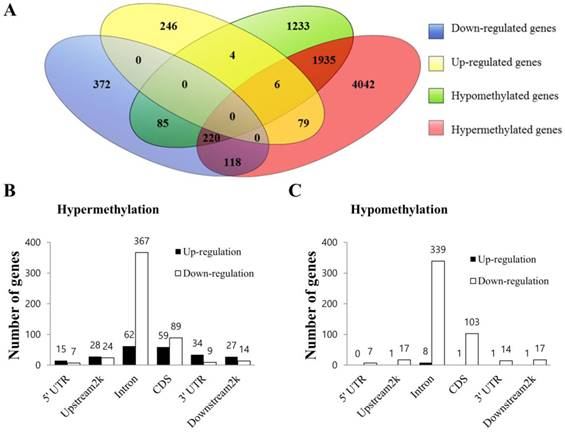
\includegraphics[width=0.8\textwidth]{journal-of-cancer_sample-result}}
%	\caption{یک نمونه نمودار خلاصه برای نمایش نوآوری در نتایج
%		%\cite{kim2016integrated}
%	}
%	\label{fig:sampleDiagram}
%\end{figure}\\
%طبیعتاً به صلاحدید نگارنده، شکل‌ها و نمودار‌ها می توانند در بخش های مختلف، خصوصا فصل
%\ref{chap:results}
%مورد استفاده قرار گیرند.
%
%\subsection{تعریف واژه‌ها (اختیاری)}
%در این قسمت محقق باید واژه‌هایی را که ممکن است برای خواننده آشنا نباشد، تعریف کند.
%
%\subsection{خلاصه فصل‌ها}
%در آخرین قسمتِ فصل اول پایان‌نامه، خلاصه‌ای اشاره‌وار از فصل‌های آتی آورده می‌شود تا خواننده بتواند تصویری واضح از دیگر قسمت‌های پایان‌نامه در ذهن خود ترسیم کند.
%
%\section{جمع‌بندی}
%در این فصل به دو مقولهٔ نحوه استفاده از قالب \پ دانشگاه تهران و نیز ویژگی‌هایی که محتویات فصل اول پایان‌نامه (یعنی مقدمه) باید داشته باشند، پرداخته شد. با توجه به اینکه این راهنما نحوه استفاده از قالب را شرح داده، ملزومات محتوایی هر فصل پایان‌نامه را توضیح می‌دهد و در پیوست‌ها نیز نحوهٔ کار با لاتک را یادآوری خواهد کرد، بنابراین مطالعهٔ کامل آن مقداری وقت شما را خواهد گرفت؛ اما مطمئن باشید از اتلاف وقت شما در ادامه کارتان تا حد زیادی جلوگیری خواهد کرد. در نوشتن متن حاضر سعی شده است علاوه بر ایجاد یک قالب لاتک برای پایان‌نامه‌های دانشگاه تهران، نکات محتوایی هر فصل نیز گوشزد گردد. طبیعتاً برای نگارش پایان‌نامهٔ خود می‌بایست مطالب تمام فصل‌ها را خودتان بازنویسی کنید.
%
%در ادامهٔ این راهنما، تنها فصل‌هایی که یک پایان‌نامه باید داشته باشد و نیز خصوصیات یا ساختاری که محتویات هر فصل باید از آنها برخوردار باشد%
%\footnote{از روی فایل «تمپلیت نگارش و تدوین پایان‌نامه \cite{UTThesisGuide}»}،
%آورده می‌شوند. نهایتاً  در پیوست‌ها، مطالبی در باب یادآوری دستورات لاتک، نحوه نوشتن فرمول‌ها، تعاریف، قضایا، مثال‌ها، درج تصاویر، نمودارها، جداول و الگوریتم‌ها و نیز مدیریت مراجع، آمده است.
%
%همچنین توصیه اکید دارم که رفع خطاهایی که احتمالاً با آنها مواجه می‌شوید را به آخر موکول نفرمایید و به محض برخورد با خطا، آن را اشکال‌زدایی و برطرف نمائید.		% فصل اول: مقدمه
% !TeX root=../main.tex
\chapter{پیشینه پژوهش}
%\thispagestyle{empty} 
\section{تولید آزمایه به صورت خودکار}
تولید خودکار آزمایه 
\LTRfootnote{Testcase}
به معنای ایجاد سناریوهای آزمون به صورت خودکار، بدون نیاز به دخالت دستی است. در این روش آزمونگر از تکنیک‌ها و ابزارهای ویژه‌ای استفاده می‌کند تا سناریوهای متنوعی برای آزمون نرم‌افزار تحت آزمون
\LTRfootnote{System Under Test}
 ایجاد کند. مزایای این روش عبارت‌اند از:
\begin{itemize}
	\item \textbf{پوشش گسترده‌تر آزمون:} تولید خودکار آزمایه‌ها، مواردی را پوشش می‌دهد که ممکن است در آزمون‌های دستی نادیده گرفته شوند. این امر به ویژه در آزمون نرم‌افزارهای پیچیده و بزرگ اهمیت بیشتری دارد.
	\item \textbf{افزایش کارایی آزمون:} با خودکارسازی فرآیند تولید آزمایه‌ها، می‌توان تعداد زیادی آزمایه در مدت زمان کوتاهی ایجاد کرد، که این کارایی در فازهای توسعه و نگهداری نرم‌افزار بسیار مفید است.
	\item \textbf{کشف باگ‌های ناشناخته:} تولید خودکار آزمایه‌ها به شناسایی باگ‌هایی کمک می‌کند که ممکن است در سناریوهای پیش‌بینی‌نشده رخ دهند. آزمون‌های تصادفی به خصوص در این زمینه بسیار مؤثر هستند.
	\item \textbf{کاهش دخالت انسانی:} خودکارسازی تولید آزمایه‌ها باعث کاهش خطاهای انسانی می‌شود و دقت و اطمینان آزمون‌ها را افزایش می‌دهد.
\end{itemize}

\section{آزمون تصادفی}
آزمون تصادفی \LTRfootnote{Random Testing} یک روش آزمون نرم‌افزار جعبه سیاه\LTRfootnote{Black Box Testing} است که در آن سیستم تحت آزمون با ورودی‌های تولید شده به صورت تصادفی ارزیابی می‌شود. هدف اصلی آزمون تصادفی، شناسایی اشکالات نرم‌افزار و اطمینان از قابلیت اطمینان و استحکام نرم‌افزار در مواجهه با انواع مختلف سناریوهای ورودی است.
\subsection{فرآیند تولید آزمایه توسط آزمون تصادفی}
فرآیند تولید آزمایه به صورت خودکار توسط روش آزمون تصادفی را می‌توان به صورت زیر ترسیم کرد:

\begin{enumerate}
	\item \textbf{تعریف فضای ورودی\LTRfootnote{Input Domain}:} در این مرحله محدوده و نوع ورودی‌هایی که نرم‌افزار می‌تواند بپذیرد، مشخص می‌گردد. این شامل تعیین دامنه‌های ورودی و محدودیت‌ها برای اطمینان از صحت موارد آزمون تولید شده است.
	\item \textbf{تولید موارد آزمون:} مجموعه‌ای از مقادیر ورودی به صورت تصادفی در داخل فضای ورودی تعریف شده تولید می‌شود. این ورودی‌ها باید طیف گسترده‌ای از سناریوهای ممکن را پوشش دهند تا احتمال کشف اشکالات افزایش یابد.
	\item \textbf{اجرای آزمون:} نرم‌افزار با استفاده از ورودی‌های تولید شده تصادفی اجرا شده و رفتار و خروجی‌های آن برای هر گونه ناهنجاری یا نتایج غیرمنتظره نظارت می‌شود.
	\item \textbf{ارزیابی خروجی‌ها:} خروجی‌های واقعی نرم‌افزار با خروجی‌های مورد انتظار (در صورت موجود بودن) مقایسه می‌شوند تا هر گونه تفاوت شناسایی گردد. در مواردی که خروجی مورد انتظار از پیش تعیین نشده است، از روش‌های اکتشافی یا اوراکل‌ها
		\LTRfootnote{Oracle}
	 برای ارزیابی درستی رفتار سیستم تحت آزمون استفاده می‌شود.
	\item \textbf{شناسایی و تحلیل اشکالات:} هر گونه انحراف یا خرابی که در حین آزمون شناسایی شود، تحلیل می‌گردد تا علل زیربنایی آن تشخیص داده شود.
\end{enumerate}


\subsection{مزایای آزمون تصادفی}
آزمون تصادفی چندین مزیت دارد که آن را به یک تکنیک ارزشمند در آزمون نرم‌افزار تبدیل می‌کند:
\begin{itemize}
	\item \textbf{سادگی:} این روش به سادگی قابل پیاده‌سازی است و نیازی به دانش عمیق از ساختار داخلی نرم‌افزار ندارد. موارد آزمون می‌توانند به صورت خودکار و بدون تلاش دستی، به صورت نامحدود تولید شوند.
	\item \textbf{خودکارسازی:} آزمون تصادفی می‌تواند به طور کامل خودکار شود و امکان آزمون پیوسته و بدون نیاز به نظارت انسانی را فراهم کند. این امر نیاز به دخالت انسانی را کاهش می‌دهد.
	\item \textbf{پوشش گسترده:} با تولید مجموعه‌ای متنوع از ورودی‌های تصادفی، آزمون تصادفی می‌تواند طیف گسترده‌ای از سناریوهای ورودی را پوشش دهد. این امر احتمال کشف اشکالات نادر یا غیرمنتظره‌ای که ممکن است از طریق دیگر روش‌های آزمون نرم‌افزار شناسایی نشوند را افزایش می‌دهد.
\end{itemize}

\subsection{معایب آزمون تصادفی}
با وجود مزایای آن، آزمون تصادفی چندین محدودیت دارد که می‌تواند بر اثربخشی آن تأثیر بگذارد:
\begin{itemize}
	\item \textbf{ناکارآمدی:} این روش می‌تواند از نظر زمان و منابع محاسباتی ناکارآمد باشد. بسیاری از ورودی‌های تولید شده ممکن است موارد آزمون معناداری را تحریک نکنند، که منجر به هدر رفتن تلاش‌ها و منابع استفاده شده جهت آزمون می‌شود.
	\item \textbf{تکرارپذیری:} آزمون تصادفی ممکن است موارد آزمون تکراری تولید کند که ارزش افزوده زیادی ندارند. نبود تمرکز بر نواحی بحرانی می‌تواند منجر به حجم بالای آزمون‌ها با نرخ شناسایی اشکال پایین شود.
	\item \textbf{تمرکز محدود:} آزمون تصادفی نواحی ورودی خاص یا نقاط خرابی بحرانی را اولویت‌بندی نمی‌کند. بنابراین، ممکن است اشکالات مهمی که در نواحی کمتر آزمون شده متمرکز شده‌اند را نادیده بگیرد.
\end{itemize}

%===============================================================================================================

\section{آزمون تصادفی تطبیقی}
آزمون تصادفی تطبیقی \LTRfootnote{Adaptive Random Testing}  با هدف بهبود آزمون تصادفی سنتی به وجود آمد و به ناکارآمدی‌ها و محدودیت‌های آن پرداخت. مفهوم آزمون تصادفی تطبیقی برای افزایش قابلیت‌های شناسایی اشکال آزمون تصادفی، با استفاده از استراتژی‌های تطبیقی که انتخاب موارد آزمون را هدایت می‌کنند، معرفی شد. آزمون تصادفی تطبیقی هدف دارد تا نرخ شناسایی اشکال بهتر را با حفظ مزایای سادگی و خودکارسازی آزمون تصادفی، بیشتر کند.

\subsection{فرضیه اصلی آزمون تصادفی تطبیقی}

توسعه آزمون تصادفی تطبیقی به دلیل نیاز به کاهش تکرارپذیری و ناکارآمدی مرتبط با تولید موارد آزمون به صورت تصادفی خالص به وجود آمد. محققان مشاهده کردند که اشکالات نرم‌افزار تمایل دارند در برخی نواحی فضای ورودی متمرکز شوند و به عبارت دیگر \textbf{نقاط خطا و شکست درون دامنه ورودی به صورت ناحیه‌ای هستند و تمایل به پیوسته بودن دارند.} در نتیجه هر چه تراکم آزمایه‌ها روی دامنه ورودی بیشتر باشد، احتمال کشف خطای جدید بیشتر خواهد بود. آزمون تصادفی تطبیقی از این مشاهده بهره می‌برد و از بازخورد موارد آزمون قبلی برای هدایت تولید موارد آزمون بعدی استفاده می‌کند. به طور کلی، آزمون تصادفی تطبیقی، آزمون تصادفی سنتی را با استفاده از تکنیک‌هایی که توزیع یکنواخت‌تری از موارد آزمون را در سراسر فضای ورودی تضمین می‌کنند، تقویت می‌کند. اصل کلیدی روش آزمون تصادفی تطبیقی این است که حداکثر تنوع موارد آزمون را به دست آورد و به این ترتیب، احتمال شناسایی خطا را افزایش دهد.

\subsection{فرآیند تولید آزمایه توسط آزمون تصادفی تطبیقی}

فرآیند تولید آزمایه به صورت خودکار توسط روش آزمون تصادفی تطبیقی را می‌توان به صورت زیر ترسیم کرد:
\begin{itemize}
	\item \textbf{تولید مجموعه کاندید\LTRfootnote{Candidate Set}:} در این مرحله ابتدایی، یک مجموعه‌ای از آزمایه‌ها با استفاده از روش آزمون تصادفی تولید می‌شود. این آزمایه‌ها به صورت تصادفی روی فضای ورودی تعریف شده از نرم‌افزار ایجاد می‌شوند.
	\item \textbf{انتخاب آزمایه:} از مجموعه کاندید تولید شده، یک آزمایه بر اساس یک استراتژی خاص که منحصراً به روش آزمون تصادفی تطبیقی مربوط است، انتخاب می‌شود. این استراتژی معمولاً به منظور به حداکثر رساندن فاصله آزمایه‌ها در فضای ورودی عمل می‌کند. با انتخاب آزمایه‌هایی که به طور گسترده‌تری پراکنده شده‌اند، آزمون تصادفی تطبیقی سعی دارد که احتمال کشف خطاها را نسبت به آزمون تصادفی سنتی افزایش دهد.
	\item \textbf{تکرار:} آزمایه انتخاب شده به مجموعه آزمایه‌های انتخاب شده \LTRfootnote{Executed Set}اضافه می‌شود و مراحل فوق به صورت تکراری انجام می‌شود. فرآیند تولید یک مجموعه کاندید جدید و انتخاب یک آزمایه ادامه می‌یابد تا زمانی که شرط خاتمه ارضاء شود که برای مثال شرط خاتمه می‌تواند رسیدن به تعداد مشخصی آزمایه باشد.
\end{itemize}
با دنبال کردن این مراحل، آزمون تصادفی تطبیقی تلاش می‌کند تا با تمرکز بر توزیع یکنواخت‌تر آزمایه‌ها، قابلیت کشف خطا را در مقایسه با آزمون تصادفی سنتی بهبود بخشد.

\subsection{مزایای آزمون تصادفی تطبیقی}
آزمون تصادفی تطبیقی چندین مزیت دارد که آن را به جایگزینی برتر برای آزمون تصادفی سنتی تبدیل می‌کند. در ادامه به برخی از این مزیت‌ها اشاره شده است:
\begin{itemize}
	\item \textbf{کاهش تکرارپذیری:} آزمون تصادفی تطبیقی با تولید موارد آزمون متنوع تکرارپذیری را کاهش می‌دهد. این امر ارزش هر مورد آزمون را به حداکثر می‌رساند و تلاش‌های بیهوده آزمون را به حداقل می‌رساند.
	\item \textbf{افزایش کارایی و نرخ شناسایی اشکال بالاتر:}‌ به دنبال کاهش تکرارپذیری موارد آزمون، کارایی روش آزمون تصادفی تطبیقی افزایش می‌یابد و فرآیند آزمون را بهبود می‌بخشد، که این خود منجر به نرخ شناسایی اشکال بالاتر با تعداد آزمایه کمتر می‌شود.
	\item \textbf{پوشش متعادل:} روش آزمون تصادفی تطبیقی، پوشش متعادل‌تری از فضای ورودی را به دست می‌آورد و خطر نادیده گرفتن نواحی مهم را کاهش می‌دهد. این پوشش جامع، استحکام کلی نرم‌افزار را افزایش می‌دهد.
	\item \textbf{بهینه‌سازی منابع:} با بهبود کارایی تولید موارد آزمون، آزمون تصادفی تطبیقی از منابع محاسباتی و زمانی بهینه استفاده می‌کند. این امر آزمون تصادفی تطبیقی را به یک راه‌حل عملی و مقیاس‌پذیر برای آزمون نرم‌افزار در مقیاس بزرگ تبدیل می‌کند.
\end{itemize}

\subsection{سربار محاسباتی پیاده سازی آزمون تصادفی تطبیقی}
در مرحله انتخاب آزمایه از فرآیند پیاده‌سازی روش آزمون تصادفی تطبیقی، لازم است که فاصله بین هر آزمایه درون مجموعه کاندید و هر آزمایه درون مجموعه آزمایه‌های انتخاب‌شده در مراحل قبلی محاسبه شود. آزمایه‌ای که بیشترین فاصله را با مجموعه آزمایه‌های انتخاب‌شده دارد، انتخاب می‌شود. در این مرحله، تعداد محاسبات فاصله باید به اندازه‌ی (تعداد آزمایه‌های درون مجموعه کاندید × تعداد آزمایه‌های درون مجموعه آزمایه‌های انتخاب‌شده) انجام شود. با افزایش تعداد اعضای مجموعه آزمایه‌های انتخاب‌شده در هر بار تکرار فرآیند، سربار محاسباتی الگوریتم آزمون تصادفی تطبیقی افزایش می‌یابد. همچنین، تعداد اعضای درون مجموعه کاندید نیز تأثیر مستقیمی بر افزایش سربار محاسباتی الگوریتم دارد. در ادامه، استراتژی‌هایی که تاکنون برای کاهش اندازه مجموعه کاندید، کاهش تعداد آزمایه‌های درون مجموعه آزمایه‌های انتخاب‌شده در مراحل قبلی الگوریتم، و در نهایت کاهش تعداد محاسبات فاصله ارائه شده‌اند، شرح داده می‌شود.

\subsubsection{اندازه مجموعه کاندید ثابت}
اولین و پرکاربردترین استراتژی پیاده‌سازی الگوریتم آزمون تصادفی تطبیقی، استراتژی "انتخاب آزمایه از مجموعه کاندید با اندازه ثابت\LTRfootnote{Fixed Sized Candidate Set (FSCS)}" است. در این استراتژی، که توسط [نام پژوهشگر/منبع] ارائه شده است، اندازه مجموعه کاندید در کل روند اجرای الگوریتم ثابت در نظر گرفته می‌شود. بهترین مقدار برای اندازه مجموعه کاندید طبق پژوهش [نام پژوهشگر/منبع] برابر با ۱۰ اعلام شده است. البته، هر چه اندازه مجموعه کاندید را افزایش دهیم، این امر می‌تواند بر اثربخشی آزمایه‌های نهایی تأثیر داشته باشد. اما بر اساس این پژوهش، هنگامی که اندازه مجموعه کاندید از ۱۰ بیشتر باشد، میزان افزایش اثربخشی مجموعه آزمایه‌ها خیلی قابل توجه نیست.

\subsubsection{بزرگ شدن فضای آزمون در آزمون تصادفی تطبیقی}
یکی از چالش‌های اصلی و مهم در آزمون تصادفی تطبیقی، بزرگ شدن فضای آزمون است. با افزایش تعداد آزمایه‌های انتخاب شده، محاسبه فاصله هر آزمایه جدید با آزمایه‌های قبلی زمان‌بر و ناکارآمد می‌شود. این مسئله باعث افزایش پیچیدگی محاسباتی و کاهش کارایی فرآیند آزمون می‌شود. برای مقابله با این مشکل، استراتژی‌های مختلفی ارائه شده‌اند که هدف آن‌ها کاهش فضای آزمون و بهبود کارایی تولید آزمایه‌ها است.
\begin{itemize}
	\item \textbf{استراتژی فراموشی\LTRfootnote{Forgetting Strategy}:} استراتژی فراموشی به منظور مدیریت فضای آزمون و جلوگیری از بزرگ شدن بیش از حد آن استفاده می‌شود. در این روش، زمانی که مجموعه آزمایه‌های از قبل انتخاب‌شده به توزیع یکنواخت مناسبی می‌رسند، این مجموعه پاک می‌شود. با این کار، فقط آزمایه‌های جدیدتر و مرتبط‌تر در فرآیند محاسبه فاصله‌ها لحاظ می‌شوند. در این استراتژی با پاک کردن آزمایه‌های قدیمی‌تر، حجم داده‌های مورد نیاز برای محاسبه فاصله‌ها کاهش می‌یابد و محاسبات سریع‌تر و کارآمدتر انجام می‌شود. البته، احتمال از دست رفتن اطلاعات مفید از آزمایه‌های قبلی وجود دارد و همچنین معیارهای فراموشی باید به دقت تنظیم شوند تا بهترین نتیجه حاصل شود.
	
	\item \textbf{خوشه‌بندی \lr{K}-مرکز\LTRfootnote{K-means Clustering Strategy}:} خوشه‌بندی \lr{K}-مرکز یکی دیگر از استراتژی‌های کاهش فضای آزمون است. در این روش، آزمایه‌های انتخاب‌شده به خوشه‌هایی تقسیم می‌شوند و هر خوشه با یک نماینده (میانگین) که مرکز خوشه است، مشخص می‌شود. برای انتخاب آزمایه جدید، فاصله بین آزمایه‌های کاندید و نمایندگان خوشه‌ها محاسبه می‌شود. این استراتژی علاوه بر کاهش تعداد محاسبات فاصله، باعث مدیریت بهتر فضای آزمون می‌شود و فضای آزمون به صورت خوشه‌بندی‌شده نگهداری می‌شود. با این حال، این روش ممکن است پیچیدگی اجرای الگوریتم را افزایش دهد و تعیین تعداد خوشه‌ها (\lr{K}) باید به دقت انجام شود تا بهترین نتیجه حاصل شود.
	
	\item \textbf{استراتژی شبکه‌بندی\LTRfootnote{Grid Strategy}:} در این روش، فضای ورودی به سلول‌های کوچکتری تقسیم می‌شود. آزمایه‌های انتخاب‌شده در هر سلول ذخیره می‌شوند و برای انتخاب آزمایه جدید، فقط سلول‌های مجاور مورد بررسی قرار می‌گیرند. این استراتژی علاوه بر کاهش تعداد محاسبات فاصله، باعث مدیریت بهتر فضای آزمون می‌شود و فضای آزمون به صورت شبکه‌بندی‌شده نگهداری می‌شود. با این حال، این روش به پیاده‌سازی دقیق شبکه‌بندی نیاز دارد و اندازه سلول‌ها باید به دقت تنظیم شود تا بهترین نتیجه حاصل شود.

\end{itemize}

\subsection{اولین پیاده‌سازی روش آزمون تصادفی تطبیقی}
اولین پیاده‌سازی روش آزمون تصادفی تطبیقی روی برنامه‌هایی با ورودی عددی\LTRfootnote{Numerical Input Domain} انجام شد. در این پیاده‌سازی، هر آزمایه که مجموعه‌ای از ورودی‌های عددی بود، به صورت یک نقطه درون یک فضای چندبعدی (تعداد ابعاد برابر با تعداد ورودی‌ها) مدل‌سازی شد. در ادامه، این الگوریتم روی یک مثال ساده بررسی می‌شود.

فرض کنید که یک برنامه به نام \lr{Sum} دارید که دو عدد به عنوان ورودی دریافت کرده و حاصل جمع آن‌ها را برمی‌گرداند. در این الگوریتم، آزمایه‌های این برنامه روی یک فضای دوبعدی به صورت نقطه مدل خواهند شد (برای مثال، آزمایه با ورودی‌های ۱۰ و ۱۵ در فضای ورودی دوبعدی نقطه \lr{(10,15)} را تشکیل می‌دهد) و فاصله بین آن‌ها، همان فاصله اقلیدسی\LTRfootnote{Euclidean distance} بین دو نقطه در نظر گرفته می‌شود.

این روش با روش آزمون تصادفی سنتی روی چند برنامه مختلف با ورودی عددی پیاده‌سازی شد و نتایج نشان داد که این روش از روش آزمون تصادفی سنتی کارایی و عملکرد بهتری دارد.

اما مهم‌ترین مشکل این روش این بود که تنها روی برنامه‌هایی با ورودی عددی قابل پیاده‌سازی بود. با این حال، این مسئله باعث شد که زمینه پژوهشی جدیدی برای محققان ایجاد شود تا راهکاری برای محاسبه فاصله بین دو آزمایه با ورودی‌های غیرعددی\LTRfootnote{Obejctive} ارائه دهند. در اکثر راهکارهای ارائه‌شده، تلاش بر این بوده که هر آزمایه را به عنوان یک نقطه در یک یا چند فضای چندبعدی مدل کنند و سپس با استفاده از محاسبات ریاضی رایج برای محاسبه فاصله در فضاهای چندبعدی، مانند فاصله اقلیدسی، فاصله بین دو نقطه را به دست آورده و به عنوان فاصله بین دو آزمایه ارائه دهند.

\subsection{آخرین ایده پیاده‌سازی ارائه شده برای روش آزمون تصادفی تطبیقی}
آخرین روشی که تاکنون در این حوزه توسط [نام پژوهشگر/منبع] ارائه شده است، شامل روش‌های \lr{WTClustering-ART} و \lr{TFClustering-ART} می‌باشد. در ادامه به بررسی دقیق ساختار و نحوه کارکرد هر کدام از این روش‌ها پرداخته شده است.

\subsubsection{تبدیل فرکانس }
کاهوچی و همکارانش روش‌هایی بر مبنای تبدیل فرکانس\LTRfootnote{Frequency Transform}، که قبلاً برای تبدیل رشته‌ها در جستجوی تشابه رشته‌ها استفاده می‌شد، پیشنهاد کردند. این روش یک رشته با طول تعریف‌شده را با تعداد دفعات هر کاراکتر در رشته به یک بردار فرکانس\LTRfootnote{Frequency Vector} تبدیل می‌کند. تعریف دقیق بردار فرکانس در ادامه آورده شده است.

\begin{itemize}
	\item \textbf{بردار فرکانس:}
	فرض کنید که \(\Sigma = \{m_1, m_2, \dots, m_n\}\) لیست توابع در یک برنامه فرضی باشد و \(s\) ترتیب فراخوانی توابع توسط آزمایه \(t\) باشد. حال بردار فرکانس به صورت 
	\(f(s) = \{f_1, f_2, \dots, f_n\}\)
	 تعریف خواهد شد که \(f_i\) تعداد دفعاتی است که تابع \(m_i\) در ترتیب فراخوانی توابع (\(s\)) حضور دارد.
	
	برای مثال فرض کنید که \(\Sigma = \{a, b, c, d, e\}\) و \(s = abddc\) ترتیب فراخوانی توابع در حین اجرای آزمایه \(t\) باشد. در این وضعیت، تابع \(a\) یک بار، \(b\) یک بار، \(c\) صفر بار، \(d\) دو بار و \(e\) یک بار فراخوانی شده است. در نتیجه:
	\[
	f(s) = \{1, 1, 0, 2, 1\}
	\]
	
	حال با توجه به اینکه هر آزمایه به یک لیست عددی با طول \(n\) (یک نقطه در فضای \(n\) بعدی) تبدیل شده است، اکنون می‌توان به سادگی فاصله بین آزمایه‌ها را با استفاده از محاسبه فاصله بین نقطه‌های متناظر آزمایه‌ها به دست آورد.
	
\end{itemize}

\subsubsection{تبدیل موجک}
اگرچه تبدیل فرکانس می‌تواند به راحتی آزمایه‌های شیء‌گرا را به بردارهایی برای اندازه‌گیری عدم تشابه تبدیل کند، اما فقط بر فرکانس فراخوانی توابع تمرکز می‌کند و به ترتیب فراخوانی توابع اهمیتی نمی‌دهد. از آنجایی که ترتیب واقعی فراخوانی توابع معمولاً بر نتایج اجرا تأثیر می‌گذارد، عدم تشابه محاسبه‌شده رضایت‌بخش نیست.

برای مثال، فرض کنید \(\Sigma = \{a, b, c, d, e\}\) و \(s_1 = acbe\) ترتیب فراخوانی توابع در آزمایه \(t_1\) و \(s_2 = bcae\) ترتیب فراخوانی توابع در آزمایه \(t_2\) باشد. بعد از انجام تبدیل فرکانس، دو بردار فرکانس\\ \(f(s_1) = f(s_2) = \{1, 1, 1, 0, 1\}\) به دست خواهد آمد. فاصله بین آزمایه \(t_1\) و \(t_2\) با توجه به مقایسه بردارهای فرکانس این دو آزمایه صفر است، در حالی که ترتیب فراخوانی توابع در دو آزمایه کاملاً یکسان نیست.

از این رو، روش تبدیل موجک در این مقاله ارائه شد که علاوه بر تعداد فراخوانی هر تابع، به ترتیب فراخوانی توابع نیز تا حدی اهمیت می‌دهد. تبدیل موجک\LTRfootnote{Wavelet Transform} ابزاری ریاضی است که برای تجزیه و تحلیل سیگنال‌ها و داده‌ها در حوزه زمان و فرکانس استفاده می‌شود. در این مقاله، از تبدیل موجک برای اندازه‌گیری عدم تشابه بین تست‌ کیس‌های شیءگرا استفاده می‌شود. این معیار با تجزیه و تحلیل سیگنال‌های مربوط به ویژگی‌های آزمایه‌ها، میزان تفاوت بین آن‌ها را محاسبه می‌کند. در روش
 \lr{ART\_WTClustering} 
 از موجک هار \LTRfootnote{Haar Wavelet} برای مدل‌سازی اطلاعات فرکانس و اطلاعات ترتیب فراخوانی توابع استفاده شده است. در ادامه، معیار تبدیل موجک با مثال توضیح داده شده است.

\begin{itemize}
	\item \textbf{تعریف تبدیل موجک آزمایه:}
فرض کنید \(s = m_1 m_2 \dots m_j\) ترتیب فراخوانی توابع باشد. \(s_1\) یک زیررشته از \(s\) است که حاوی نیمه اول عناصر \(s\) است و \(s_2\) یک زیررشته دیگر از \(s\) است که حاوی نیمه دوم عناصر \(s\) است. تبدیل موجک \(s\) به صورت \(W(s) = [A, B]\) تعریف می‌شود که \(A = f(s)\) و \(B = B_1 - B_2\) که \(B_1 = f(s_1)\) و \(B_2 = f(s_2)\) است.

برای مثال فرض کنید که \(\Sigma = \{a, b, c, d, e\}\) و \(s = abdde\) ترتیب فراخوانی توابع در حین اجرای آزمایه \(t\) باشد. حال مقادیر \(A\) , \(B\) و \(W(s)\) به صورت زیر محاسبه خواهند شد:
\begin{align*}
	A = f(s) &= \{1, 1, 0, 2, 1\} \\
	s_1 = ab \quad & \Rightarrow \quad B_1 = \{1, 1, 0, 0, 0\} \\
	s_2 = dde \quad &\Rightarrow \quad B_2 = \{0, 0, 0, 2, 1\} \\
	B = B_1 - B_2 \quad &\Rightarrow \quad B = \{1, 1, 0, -2, -1\} \\
	W(s) = [A, B] \quad &\Rightarrow \quad W(s) = \left[\{1, 1, 0, 2, 1\}, \{1, 1, 0, -2, -1\}\right]
\end{align*}

\item \textbf{محاسبه فاصله بین آزمایه‌‌ها:}
فرض کنید \(\Sigma = \{m_1, m_2, \dots, m_n\}\) لیست توابع درون یک برنامه فرضی باشد. اگر \(s_1\) ترتیب فراخوانی توابع توسط آزمایه \(t_1\) و \(s_2\) ترتیب فراخوانی توابع توسط آزمایه \(t_2\) باشد، آنگاه \(W(s_1) = [A_1, B_1]\) و \(W(s_2) = [A_2, B_2]\) خواهد بود که \(A_1 = \{A_{11}, A_{12}, \dots, A_{1n}\}\) و \(B_1 = \{B_{11}, B_{12}, \dots, B_{1n}\}\) و \(A_2 = \{A_{21}, A_{22}, \dots, A_{2n}\}\) و \(B_2 = \{B_{21}, B_{22}, \dots, B_{2n}\}\) که فاصله \(WT\_D\) بین این دو آزمایه به صورت زیر محاسبه خواهد شد:
\[
WT\_D(t_1, t_2) = \sqrt{\sum_{i=1}^{n} (A_{1i} - A_{2i})^2} + \sqrt{\sum_{i=1}^{n} (B_{1i} - B_{2i})^2}
\]


\end{itemize}

\subsubsection{تبدیل فرکانس سه‌بخشی}
تا حدی، استفاده مستقیم از تبدیل موجک برای آزمایه‌های شیءگرا نامناسب است. دلیل اصلی این است که، اگرچه دنباله فراخوانی توابع را به دو قسمت تقسیم می‌کند و آنها را حفظ می‌کند، اما تنها تفریق نیمه اول و دوم این دنباله نمی‌تواند تفاوت بین توالی فراخوانی توابع را نمایش دهد. برای پرداختن به این موضوع، در این مقاله پیشنهاد شده است که از تبدیل فرکانس سه‌بخشی \LTRfootnote{Trisection Frequency Conversion (TFC)} استفاده شود. این معیار نه تنها به تعداد فراخوانی هر تابع در حین اجرای آزمایه‌ها توجه دارد بلکه ترتیب فراخوانی توابع در حین اجرای آزمایه‌های مختلف نیز اهمیت دارد.

\begin{itemize}

\item \textbf{تعریف معیار تبدیل فرکانس سه‌بخشی:}
فرض کنید که \(s = m_1 m_2 \dots m_j\) ترتیب فراخوانی توابع در حین اجرای آزمایه \(t\) باشد و \(s_1\) نیمه اول \(s\) و \(s_2\) نیمه دوم \(s\) باشد. معیار تبدیل فرکانس سه‌بخشی برای \(s\) به صورت \(TF(s) = [A, B, C]\) نمایش داده می‌شود که \(A = f(s)\)، \(B = f(s_1)\) و \(C = f(s_2)\) است.

\item \textbf{محاسبه فاصله بین آزمایه‌‌ها:}

فرض کنید \(\Sigma = \{m_1, m_2, \dots, m_n\}\) لیست توابع در یک برنامه فرضی باشد. یک آزمایه \(t_1\) با دنباله فراخوانی توابع \(s_1\) و یک آزمایه \(t_2\) با دنباله فراخوانی توابع \(s_2\) را در نظر بگیرید. فرض کنید\\ \(TF(s_1) = [A_1, B_1, C_1]\) و \(TF(s_2) = [A_2, B_2, C_2]\) که در آن \(A_1 = \{A_{11}, A_{12}, \dots, A_{1n}\}\)، \(B_1 = \{B_{11}, B_{12}, \dots, B_{1n}\}\)، \(C_1 = \{C_{11}, C_{12}, \dots, C_{1n}\}\)، \(A_2 = \{A_{21}, A_{22}, \dots, A_{2n}\}\)، \(B_2 = \{B_{21}, B_{22}, \dots, B_{2n}\}\)، و \(C_2 = \{C_{21}, C_{22}, \dots, C_{2n}\}\). تفاوت ترتیب بین \(s_1\) و \(s_2\) به صورت \(\sum_{i=1}^{j} \left(1 - \delta_{s_{1i} s_{2i}}\right)\) تعریف می‌شود، که \(\delta_{s_{1i} s_{2i}}\) نماد دلتای کرونکر استاندارد است، به طوری که اگر \(s_{1i} = s_{2i}\) باشد آنگاه \(\delta_{s_{1i} s_{2i}} = 1\) و در غیر اینصورت \(\delta_{s_{1i} s_{2i}} = 0\). فاصله \(TFC\)  یا \(TFC\_D\) بین این دو آزمایه به صورت زیر تعریف می‌شود:

\[
TFC\_D(t_1, t_2) = \sqrt{\sum_{i=1}^{n} (A_{1i} - A_{2i})^2} + \sqrt{\sum_{i=1}^{n} (B_{1i} - B_{2i})^2}
\]
\[
+ \sqrt{\sum_{i=1}^{n} (C_{1i} - C_{2i})^2} + \sum_{i=1}^{n} \left(1 - \delta_{s_{1i} s_{2i}}\right)
\quad
\]

\end{itemize}

\subsubsection{مقایسه بین \(TFC\_D\) و \(WT\_D\):}
در اینجا به بررسی تفاوت‌های \(WT\_D\) و \(TFC\_D\) در یک مثال پرداخته شده است. دو آزمایه \(t_1\) و \(t_2\) را در نظر بگیرید که ترتیب فراخوانی توابع توسط این دو آزمایه به صورت \(s_1 = abce\) و \(s_2 = abec\) است که \(s_{11} = ab\)، \(s_{12} = ce\)، \(s_{21} = ab\) و \(s_{22} = ec\) است. در نتیجه:

\begin{align*}
	W(s_1) &= \left[\langle 1, 1, 1, 0, 1 \rangle, \langle 1, 1, -1, 0, -1 \rangle \right] \\
	W(s_2) &= \left[\langle 1, 1, 1, 0, 1 \rangle, \langle 1, 1, -1, 0, -1 \rangle \right]
\end{align*}

است و در نتیجه \({WT\_D}(s_1, s_2)\) برابر است با:

\[
WT\_D(s_1, s_2) = \sqrt{0^2 + 0^2 + 0^2 + 0^2 + 0^2} + \sqrt{0^2 + 0^2 + 0^2 + 0^2 + 0^2} = 0
\]
\textbf{}
از طرفی با توجه به تعریف \(TF(s_i)\) مقادیر \(TF(s_1)\) و \(TF(s_2)\) و \(TFC\_D(s_1, s_2)\) به صورت زیر محاسبه می‌شوند:
\[
TF(s_1) = \left[\langle 1, 1, 1, 0, 1 \rangle, \langle 1, 1, 0, 0, 0 \rangle, \langle 0, 0, 1, 0, 1 \rangle\right]
\]
\[
TF(s_2) = \left[\langle 1, 1, 1, 0, 1 \rangle, \langle 1, 1, 0, 0, 0 \rangle, \langle 0, 0, 1, 0, 1 \rangle\right]
\]

\(TFC\_D(s_1, s_2)\) به صورت زیر محاسبه می‌شود:

\begin{align*}
	TFC\_D(s_1, s_2) &= \sqrt{0^2 + 0^2 + 0^2 + 0^2 + 0^2} + \sqrt{0^2 + 0^2 + 0^2 + 0^2 + 0^2} \\
	&\quad + \sqrt{0^2 + 0^2 + 0^2 + 0^2 + 0^2} + \sum_{i=1}^{j} \left(1 - \delta_{s_{1i}s_{2i}}\right)
\end{align*}

که

\[
\sum_{i=1}^{j} \left(1 - \delta_{s_{1i}s_{2i}}\right) = (1-1) + (1-1)  + (1-0)  + (1-0) = 2
\]

بنابراین:

\[
TFC\_D(s_1, s_2) = 0 + 0 + 0 + 2 = 2 
\]

همانطور که مشاهده کردید،‌ فاصله \(TFC\) در این مثال نسبت به فاصله \(ٌُWT\)  به ترتیب فراخوانی توابع توسط آزمایه‌ها اهمیت بیشتری می دهد.


\newpage

	\begin{tikzpicture}[node distance=2.5cm]
		
		\node (start) [startstop] {\rl{به صورت تصادفی اولین مورد آزمایشی شئ‌گرا را ایجاد کرده و اجرا کنید}};
		\node (decision) [decision, below of=start, yshift=-1cm] {\rl{شرط خاتمه}};
		\node (output) [startstop, right of=decision, xshift=4cm] {\rl{خروجی آزمایه‌های تولید شده}};
		\node (process1) [process, below of=decision, yshift=-1cm] {\rl{اضافه کردن این آزمایه به مجموعه آزمایه‌های انتخاب شده در مراحل قبلی الگوریتم}};
		\node (process2) [process, below of=process1, yshift=-1cm] {\rl{تولید ۱۰ آزمایه شئ‌گرا جدید به عنوان مجموعه کاندید}};
		
		\node (process3) [process, below of=process2, yshift=-1cm, xshift=0.5cm, text width=7cm] {\rl{خوشه‌بندی مجموعه آزمایه‌های از قبل انتخاب شده به \rl{K} خوشه}};
		\node (process4) [process, below of=process3, yshift=-0.5cm] {\rl{تعیین نماینده هر خوشه برای ارزیابی آزمایه‌های کاندید}};
		\node (process5) [process, below of=process4, yshift=-0.5cm] {Select the candidate which has the smallest distance with the subset};
		
		\draw [arrow] (start) -- (decision);
		\draw [arrow] (decision) -- node[anchor=east] {No} (process1);
		\draw [arrow] (decision) -- node[anchor=north] {Yes} (output);
		\draw [arrow] (process1) -- (process2);
		\draw [arrow] (process2) -- (process3);
		\draw [arrow] (process3) -- (process4);
		\draw [arrow] (process4) -- (process5);
%		\draw [arrow] (process5.east) -| ++(4,0) |- (decision.east);
		
		% Adding labels ①, ②, ③
%		\node[draw=none, fill=none] at ($(process2)!0.5!(process3)$) {\textcircled{1}};
%		\node[draw=none, fill=none] at ($(process3)!0.5!(process4)$) {\textcircled{2}};
%		\node[draw=none, fill=none] at ($(process4)!0.5!(process5)$) {\textcircled{3}};
		
	\end{tikzpicture}



\subsection{روش‌های مختلف انتخاب آزمایه بر اساس فاصله}


\subsection{نقطه اشتراک اکثر روش‌های پیاده‌سازی الگوریتم آزمون تصادفی تطبیقی}

\section{روش تقسیم‌بندی فضای ورودی}

\subsection{فرآیند تولید آزمایه توسط روش تقسیم‌بندی فضای ورودی}

%===============================================================================================================




%
%
%
%\newpage
%\section{مقدمه}
%هدف از این فصل که با عنوان‌های  «مروری بر ادبیات موضوع%
%\LTRfootnote{Literature Review}»،
%«مروری بر منابع» و یا «مروری بر پیشینه تحقیق%
%\LTRfootnote{Background Research}»
%معرفی می‌شود، بررسی و طبقه‌بندی یافته‌های تحقیقات دیگر محققان در سطح دنیا و تعیین و شناسایی خلأهای تحقیقاتی است. آنچه را که تحقیق شما به دانش موجود اضافه می‌کند، مشخص کنید. طرح پیشینه تحقیق%
%\LTRfootnote{Background Information}
%یک مرور محققانه است و تا آنجا باید پیش برود که پیش‌زمینهٔ تاریخی مناسبی از تحقیق را بیان کند و جایگاه تحقیق فعلی را در میان آثار پیشین نشان دهد. برای این منظور منابع مرتبط با تحقیق را بررسی کنید، البته نه آنچنان گسترده که کل پیشینه تاریخی بحث را در برگیرد. برای نوشتن این بخش:
%\begin{itemize}
%	\item
%	دانستنی‌های موجود و پیش‌زمینهٔ تاریخی و وضعیت کنونی موضوع را چنان بیان کنید که خواننده بدون مراجعه به منابع پیشین، نتایج حاصل از مطالعات قبلی را درک و ارزیابی کند.
%	\item
%	نشان دهید که بر موضوع احاطه دارید. پرسش تحقیق را همراه بحث و جدل‌ها و مسائل مطرح شده بیان کنید و مهم‌ترین تحقیق‌های انجام شده در این زمینه را معرفی نمائید.
%	\item
%	ابتدا مطالب عمومی‌تر و سپس پژوهش‌های مشابه با کار خود را معرفی کرده و نشان دهید که تحقیق شما از چه جنبه‌ای با کار دیگران تشابه یا تفاوت دارد.
%	\item
%	اگر کارهای قبلی را خلاصه کرده‌اید، از پرداختن به جزئیات غیرضروری بپرهیزید. در عوض، بر یافته‌ها و مسائل روش‌شناختی مرتبط و نتایج اصلی تأکید کنید و اگر بررسی‌ها و منابع مروری عمومی دربارهٔ موضوع موجود است، خواننده را به آنها ارجاع دهید.
%\end{itemize}
%
%\section{تعاریف، اصول و مبانی نظری}
%این قسمت ارائهٔ خلاصه‌ای از دانش کلاسیک موضوع است. این بخش الزامی نیست و بستگی به نظر استاد راهنما دارد.
%
%\section{مروری بر ادبیات موضوع}
%در این قسمت باید به کارهای مشابه دیگران در گذشته اشاره کرد و وزن بیشتر این قسمت بهتر است به مقالات ژورنالی سال‌های اخیر (۲ تا ۳ سال) تخصیص داده شود. به نتایج کارهای دیگران با ذکر دقیق مراجع باید اشاره شده و جایگاه و تفاوت تحقیق شما نیز با کارهای دیگران مشخص شود. استفاده از مقالات ژورنال‌های معتبر در دو یا سه سال اخیر، می‌تواند به اعتبار کار شما بیافزاید.
%
%\section{نتیجه‌گیری}
%‌در نتیجه‌گیری آخر این فصل، با توجه به بررسی انجام شده بر روی مراجع تحقیق، بخش‌های قابل گسترش و تحقیق در آن حیطه و چشم‌اندازهای تحقیق مورد بررسی قرار می‌گیرند.	در برخی از تحقیقات، نتیجه نهایی فصل روش تحقیق، ارائهٔ یک چارچوب کار تحقیقی 
%\lr{(research framework)}
است.		% فصول دوم: مروری بر مطالعات انجام شده
% !TeX root=../main.tex
\chapter{پیشینه پژوهش}\label{chapter3}
%\thispagestyle{empty} 

\section{آزمون تصادفی}
آزمون تصادفی
\cite{hamlet1994random}
 یک روش آزمون نرم‌افزار جعبه سیاه
\LTRfootnote{Black Box Testing}
  است که در آن سیستم تحت آزمون با ورودی‌های تولید شده به صورت تصادفی ارزیابی می‌شود. هدف اصلی آزمون تصادفی، شناسایی اشکالات نرم‌افزار و اطمینان از کیفیت و استحکام نرم‌افزار در مواجهه با انواع مختلف سناریوهای ورودی است. تاکنون از روش آزمون تصادفی برای آزمون سیستم‌های مختلفی همچون برنامه‌های سیستم‌عامل مَک~\LTRfootnote{macos}\cite{miller2006empirical}
 ، سیستم‌های نرم‌افزاری توزیع‌شده~\LTRfootnote{Embedded Software Systems}\cite{regehr2005random}
  ، سیستم‌های پایگاه‌داده اس‌ کیو ال~\LTRfootnote{SQL}\cite{bati2007genetic}
  و برنامه‌های اندرویدی~\LTRfootnote{Android Applications}\cite{muangsiri2017random}
استفاده شده است.
\newpage
\subsection{فرآیند تولید آزمایه توسط آزمون تصادفی}

فرآیند تولید آزمایه به صورت خودکار توسط روش آزمون تصادفی را می‌توان به صورت زیر ترسیم کرد:

\begin{enumerate}
	\item \textbf{تعریف فضای ورودی\LTRfootnote{Input Domain}}
	
	 در این مرحله محدوده و نوع ورودی‌هایی که نرم‌افزار می‌تواند بپذیرد، مشخص می‌گردد. این مرحله شامل تعیین دامنه‌های ورودی و محدودیت‌ها برای اطمینان از صحت آزمایه‌های تولید شده است.
	\item \textbf{تولید آزمایه}
	
	 مجموعه‌ای از مقادیر ورودی به صورت تصادفی در داخل فضای ورودی تعریف شده، تولید می‌شود. این ورودی‌ها باید طیف گسترده‌ای از سناریوهای ممکن را پوشش دهند تا احتمال کشف اشکالات سیستم تحت آزمون افزایش یابد.
	\item \textbf{اجرای آزمایه‌ها}
	
	 نرم‌افزار با استفاده از ورودی‌های تصادفی تولید شده اجرا شده و رفتار و خروجی‌های آن برای هر گونه ناهنجاری یا نتایج غیرمنتظره نظارت می‌شود.
	\item \textbf{ارزیابی خروجی‌ها}
	
	 خروجی‌های واقعی نرم‌افزار با خروجی‌های مورد انتظار (در صورت موجود بودن) مقایسه می‌شوند تا هر گونه تفاوت شناسایی گردد. در مواردی که خروجی مورد انتظار از پیش تعیین نشده است، می‌توان از روش‌های اکتشافی یا اوراکل‌ها~\LTRfootnote{Oracle}\cite{nardi2015survey}
	 برای ارزیابی درستی رفتار سیستم تحت آزمون استفاده کرد.
	\item \textbf{شناسایی و تحلیل اشکالات}
	
	 هر گونه اشکال و مغایرت خروجی سیستم با خروجی مورد انتظار که در حین آزمون شناسایی شود، تحلیل می‌گردد تا علل زیربنایی آن تشخیص داده شود.
	 
\end{enumerate}

\subsection{مزایای آزمون تصادفی}
آزمون تصادفی چندین مزیت دارد که آن را به یک تکنیک ارزشمند در آزمون نرم‌افزار تبدیل می‌کند. در ادامه به چند مورد از مزیت‌های آزمون تصادفی اشاره شده است.
\begin{itemize}
	\item \textbf{پوشش گسترده}
	
	با تولید مجموعه‌ای متنوع از ورودی‌های تصادفی، آزمون تصادفی می‌تواند طیف گسترده‌ای از سناریوهای ورودی را پوشش دهد. این امر احتمال کشف اشکالات نادر یا غیرمنتظره‌ای که ممکن است از طریق دیگر روش‌های آزمون نرم‌افزار شناسایی نشوند را افزایش می‌دهد.
	\item \textbf{سادگی}
	
	 این روش به سادگی قابل پیاده‌سازی است و نیازی به دانش عمیق از ساختار داخلی نرم‌افزار ندارد و آزمایه‌ها می‌توانند به صورت خودکار و بدون تلاش دستی، به صورت نامحدود تولید شوند.
	\item \textbf{خودکارسازی}
	
	 آزمون تصادفی می‌تواند به طور کامل خودکار شود و امکان آزمون پیوسته و بدون نیاز به نظارت انسانی را فراهم کند. این امر نیاز به دخالت انسانی را کاهش می‌دهد.

\end{itemize}

\subsection{معایب آزمون تصادفی}
با وجود مزایای آن، آزمون تصادفی چندین محدودیت دارد که می‌تواند بر اثربخشی آن تأثیر بگذارد. در ادامه به چند مورد از معایب آزمون تصادفی اشاره شده است.
\begin{itemize}
	\item \textbf{تکرارپذیری}
	
	آزمون تصادفی ممکن است آزمایه‌های تکراری تولید کند که ارزش افزوده زیادی ندارند. تکرارپذیری آزمایه‌ها می‌تواند منجر به حجم بالای آزمون‌ها با نرخ شناسایی اشکال پایین شود.
	\item \textbf{ناکارآمدی}
	
	 این روش می‌تواند از نظر زمان و منابع محاسباتی ناکارآمد باشد. بسیاری از ورودی‌های تولید شده ممکن است آزمایه‌های معناداری را تولید نکنند، که منجر به هدر رفتن تلاش‌ها و منابع استفاده شده جهت آزمون می‌شود.
	\item \textbf{تمرکز محدود}
	
	 آزمون تصادفی نواحی ورودی خاص یا نقاط خرابی بحرانی را اولویت‌بندی نمی‌کند. بنابراین، ممکن است اشکالات مهمی که در نواحی کمتر آزمون شده متمرکز شده‌اند را نادیده بگیرد.
\end{itemize}

\section{آزمون تصادفی تطبیقی}
آزمون تصادفی تطبیقی
 \cite{huang2019survey}
   با هدف بهبود آزمون تصادفی به وجود آمد و به رفع ناکارآمدی‌ها و محدودیت‌های آن پرداخت. مفهوم آزمون تصادفی تطبیقی برای افزایش قابلیت‌های شناسایی اشکال آزمون تصادفی، با استفاده از استراتژی‌های تطبیقی که انتخاب آزمایه‌ها را هدایت می‌کنند، معرفی شد. آزمون تصادفی تطبیقی هدف دارد تا نرخ شناسایی اشکال را با حفظ مزایای سادگی و خودکارسازی آزمون تصادفی، بیشتر کند.

\subsection{ریشه آزمون تصادفی تطبیقی}

توسعه آزمون تصادفی تطبیقی به دلیل نیاز به کاهش تکرارپذیری و ناکارآمدی مرتبط با تولید آزمایه‌ها به صورت تصادفی خالص به وجود آمد. محققان مشاهده کردند که اشکالات نرم‌افزار تمایل دارند در برخی نواحی فضای ورودی متمرکز شوند~\cite{white1980domain}\cite{ammann1988data}\cite{finelli1991nasa}\cite{bishopvariation}\cite{schneckenburger2007towards}
 و به عبارت دیگر \textbf{نقاط باعث شکست\LTRfootnote{Failure} درون دامنه ورودی به صورت ناحیه‌ای هستند و تمایل به پیوسته بودن دارند}.
در نتیجه، اگر نواحی باعث شکست به‌صورت پیوسته باشند، نواحی غیرشکست نیز باید در سراسر دامنه ورودی مجاور یکدیگر باشند. به‌طور خاص، اگر یک آزمایه \lr{tc} یک ورودی باعث شکست باشد، احتمال بالایی وجود دارد که همسایگان آن نیز باعث شکست شوند؛ به‌طور مشابه، اگر \lr{tc} باعث شکست نشود، احتمال بالایی وجود دارد که همسایگان آن نیز باعث شکست نشوند. به‌عبارت دیگر، یک ورودی برنامه که از ورودی‌های غیرشکست دور است، احتمال بیشتری برای شناسایی شکست نسبت به آزمایه‌های همسایه داشته باشد. از طرف دیگر، یک ورودی که به ورودی‌های باعث شکست نزدیک است، به احتمال زیاد باعث شکست خواهد شد، اما احتمال بالایی وجود دارد که ناحیه باعث شکست شناسایی‌شده توسط این ورودی، قبلاً توسط ورودی‌های باعث شکست همسایه شناسایی شده باشد و شناسایی مجدد آن سودی نخواهد داشت.

 در نتیجه هر چه تراکم آزمایه‌ها روی دامنه ورودی بیشتر باشد، احتمال کشف اشکالات جدید بیشتر خواهد بود. آزمون تصادفی تطبیقی از این مشاهده بهره می‌برد و از بازخورد آزمایه‌ها قبلی برای هدایت تولید آزمایه‌های بعدی استفاده می‌کند. به طور کلی، آزمون تصادفی تطبیقی، آزمون تصادفی را با استفاده از تکنیک‌هایی که توزیع یکنواخت‌تری از آزمایه‌ها را در سراسر فضای ورودی تضمین می‌کنند، تقویت می‌کند. اصل کلیدی روش آزمون تصادفی تطبیقی این است که حداکثر تنوع آزمایه‌ها را به دست آورد و به این ترتیب، احتمال شناسایی شکست‌های جدید را افزایش دهد\cite{chen2010adaptive}.

\subsection{فرآیند تولید آزمایه توسط آزمون تصادفی تطبیقی}

فرآیند تولید آزمایه به صورت خودکار توسط روش آزمون تصادفی تطبیقی را می‌توان به صورت زیر ترسیم کرد:
\begin{enumerate}
	\item \textbf{تولید مجموعه کاندید\LTRfootnote{Candidate Set}}
	
	 در ابتدا، یک مجموعه‌ای از آزمایه‌ها با استفاده از روش آزمون تصادفی تولید می‌شود. این آزمایه‌ها به صورت تصادفی روی فضای ورودی تعریف شده برای سیستم تحت آزمون ایجاد می‌شوند.
	 
	\item \textbf{انتخاب آزمایه}
	
	 از مجموعه کاندید تولید شده، یک آزمایه بر اساس یک استراتژی خاص که منحصراً به روش آزمون تصادفی تطبیقی مربوط است، انتخاب می‌شود. این استراتژی معمولاً به منظور به حداکثر رساندن پراکندگی آزمایه‌ها در فضای ورودی عمل می‌کند. با انتخاب آزمایه‌هایی که به طور گسترده‌تری پراکنده شده‌اند، آزمون تصادفی تطبیقی سعی دارد که احتمال کشف شکست‌ها را نسبت به آزمون تصادفی افزایش دهد. اکثر این استراتژی‌ها در ابتدا یک معیار فاصله بین آزمایه‌ها تعریف کرده‌اند و سپس با توجه به این معیار، سعی بر انتخاب آزمایه‌هایی از بین مجموعه آزمایه‌های کاندید داشته‌اند که بیشترین فاصله را با مجموعه آزمایه‌های انتخاب‌شده قبلی\LTRfootnote{Executed Set} داشته باشند.
	 
	\begin{itemize}
		\item \textbf{روش‌های مختلف انتخاب آزمایه بر اساس فاصله}
		
		تاکنون روش‌های مختلفی برای انتخاب آزمایه با توجه به فاصله‌های به دست آمده بین مجموعه آزمایه‌های کاندید و مجموعه آزمایه‌های انتخاب‌شده در مراحل قبلی الگوریتم آزمون تصادفی تطبیقی ارائه شده است. در ادامه به بررسی مهم‌ترین و مطرح‌ترین این روش‌ها پرداخته شده است.
		
		\begin{itemize}
			\item \textbf{بیشترین-کمترین فاصله\LTRfootnote{max-min distance}}
			 
			در این روش \cite{chen2001proportional} به ازای هر آزمایه درون مجموعه کاندید، فاصله با آزمایه‌های انتخاب‌شده قبلی محاسبه می‌شود و «کمترین فاصله» بین آن آزمایه کاندید و مجموعه آزمایه‌های انتخاب‌شده قبلی محاسبه می‌شود. سپس آزمایه‌ کاندیدی انتخاب می‌شود که مقدار «کمترین فاصله» آن از بقیه آزمایه‌های کاندید بیشتر باشد.
			
			\item \textbf{بیشترین-مجموع فاصله\LTRfootnote{max-sum distance}}
			 
			در این روش \cite{zhou2021cost} به ازای هر آزمایه درون مجموعه کاندید، «مجموع فاصله» با آزمایه‌های انتخاب‌شده قبلی محاسبه می‌شود و سپس آزمایه‌ای انتخاب می‌شود که مقدار «مجموع فاصله» آن از بقیه آزمایه‌های درون مجموعه کاندید بیشتر باشد.
		\end{itemize}
		
	\end{itemize}
	
	\item \textbf{تکرار}
	
	 آزمایه انتخاب شده به مجموعه آزمایه‌های انتخاب شده اضافه می‌شود و فرآیند تولید یک مجموعه کاندید جدید و انتخاب متفاوت‌ترین آزمایه تا زمانی که شرط خاتمه ارضاء شود ادامه می‌یابد. برای مثال شرط خاتمه می‌تواند رسیدن به تعداد مشخصی آزمایه یا شناسایی درون سیستم تحت آزمون باشد\cite{huang2019survey}.

\end{enumerate}
با دنبال کردن این مراحل، آزمون تصادفی تطبیقی تلاش می‌کند تا با تمرکز بر توزیع یکنواخت‌تر آزمایه‌ها، قابلیت کشف اشکال را در مقایسه با آزمون تصادفی بهبود بخشد.

\subsection{مزایای آزمون تصادفی تطبیقی}
آزمون تصادفی تطبیقی چندین مزیت دارد که آن را به جایگزینی مناسب برای آزمون تصادفی تبدیل می‌کند\cite{johansson2023comparison}. در ادامه به برخی از این مزیت‌ها اشاره شده است.
\begin{itemize}
	\item \textbf{کاهش تکرارپذیری}
	
	 آزمون تصادفی تطبیقی با تولید آزمایه‌های متنوع تکرارپذیری را کاهش می‌دهد. این امر ارزش هر مورد آزمون را به حداکثر می‌رساند و تلاش‌های بیهوده آزمون را به حداقل می‌رساند.
	\item \textbf{افزایش کارایی و نرخ شناسایی اشکال بالاتر}‌ 
	
	به دنبال کاهش تکرارپذیری آزمایه‌ها، کارایی روش آزمون تصادفی تطبیقی افزایش می‌یابد و فرآیند آزمون را بهبود می‌بخشد، که این خود منجر به نرخ شناسایی اشکال بالاتر با تعداد آزمایه کمتر می‌شود.
	\item \textbf{پوشش متعادل}
	
	 روش آزمون تصادفی تطبیقی، پوشش متعادل‌تری از فضای ورودی را به دست می‌آورد و خطر نادیده گرفتن نواحی مهم را کاهش می‌دهد. این پوشش جامع، استحکام کلی نرم‌افزار را افزایش می‌دهد.
	\item \textbf{بهینه‌سازی منابع}
	
	 با بهبود روند تولید آزمایه‌ها، آزمون تصادفی تطبیقی از منابع محاسباتی و زمانی بهینه استفاده می‌کند. این امر آزمون تصادفی تطبیقی را به یک راه‌حل عملی و مقیاس‌پذیر برای آزمون نرم‌افزار در مقیاس بزرگ تبدیل می‌کند.
\end{itemize}

\subsection{هزینه پیاده‌سازی آزمون تصادفی تطبیقی}
در مرحله انتخاب آزمایه از فرآیند پیاده‌سازی روش آزمون تصادفی تطبیقی، لازم است که فاصله بین هر آزمایه درون مجموعه کاندید و هر آزمایه درون مجموعه آزمایه‌های انتخاب‌شده در مراحل قبلی محاسبه شود. آزمایه‌ای که بیشترین فاصله را با مجموعه آزمایه‌های انتخاب‌شده دارد، انتخاب می‌شود. در این مرحله، باید (تعداد آزمایه‌های درون مجموعه کاندید × تعداد آزمایه‌های درون مجموعه آزمایه‌های انتخاب‌شده) بار فاصله محاسبه شود. با افزایش تعداد اعضای مجموعه آزمایه‌های انتخاب‌شده در هر بار تکرار فرآیند، هزینه اجرای الگوریتم آزمون تصادفی تطبیقی افزایش می‌یابد. همچنین، تعداد اعضای درون مجموعه کاندید نیز تأثیر مستقیمی بر افزایش هزینه اجرای الگوریتم دارد. در ادامه، استراتژی‌هایی که تاکنون برای کاهش اندازه مجموعه کاندید، کاهش تعداد آزمایه‌های لازم برای محاسبه فاصله با مجموعه آزمایه‌های کاندید در مجموعه آزمایه‌های انتخاب‌شده قبلی، و در نهایت کاهش تعداد محاسبات فاصله ارائه شده‌اند، شرح داده می‌شود.

\subsubsection{اندازه مجموعه کاندید ثابت}
اولین و پرکاربردترین استراتژی پیاده‌سازی الگوریتم آزمون تصادفی تطبیقی، استراتژی «انتخاب آزمایه از مجموعه کاندید با اندازه ثابت\LTRfootnote{Fixed Sized Candidate Set (FSCS)}\cite{chen2001proportional}» است و پژوهش‌های زیادی پیرو این استراتژی، تاکنون انجام شده است
\cite{chen2007test}
\cite{kuo2008enhancing}
\cite{chen2007distribution}
\cite{keele2007guidelines}. 
در این استراتژی، اندازه مجموعه کاندید در کل روند اجرای الگوریتم ثابت در نظر گرفته می‌شود. بهترین مقدار برای اندازه مجموعه کاندید طبق پژوهش \cite{chen2005adaptive} برابر با ۱۰ اعلام شده است. البته، هر چه اندازه مجموعه کاندید را افزایش دهیم، این امر می‌تواند بر اثربخشی آزمایه‌های نهایی تأثیر داشته باشد. اما بر اساس این پژوهش، هنگامی که اندازه مجموعه کاندید از ۱۰ بیشتر باشد، میزان افزایش اثربخشی مجموعه آزمایه‌های نهایی خیلی قابل توجه نیست.

\subsubsection{بزرگ شدن فضای آزمون در آزمون تصادفی تطبیقی}
یکی از چالش‌های اصلی و مهم در آزمون تصادفی تطبیقی، بزرگ شدن فضای آزمون است. با افزایش تعداد آزمایه‌های انتخاب شده، محاسبه فاصله هر آزمایه جدید با آزمایه‌های قبلی زمان‌بر و ناکارآمد می‌شود. این مسئله باعث افزایش هزینه محاسباتی و کاهش کارایی فرآیند آزمون می‌شود. برای مقابله با این مشکل، استراتژی‌های مختلفی ارائه شده‌اند که هدف آن‌ها کاهش فضای آزمون و بهبود کارایی تولید آزمایه‌ها است.
\begin{itemize}
	\item \textbf{استراتژی فراموشی\LTRfootnote{Forgetting Strategy}}
	
	 استراتژی فراموشی \cite{chan2006forgetting}\cite{mao2017out} به منظور مدیریت فضای آزمون و جلوگیری از بزرگ شدن بیش از حد آن استفاده می‌شود. در این روش، زمانی که مجموعه آزمایه‌های انتخاب‌شده قبلی به توزیع یکنواخت مناسبی می‌رسند، این مجموعه برای محاسبه میزان فاصله با مجموعه آزمایه‌های کاندید در مراحل بعدی الگوریتم در نظر گرفته نمی‌شود. با این کار، فقط آزمایه‌های جدیدتر و مرتبط‌تر در فرآیند محاسبه فاصله‌ها لحاظ می‌شوند. در این استراتژی با در نظر نگرفتن مجموعه آزمایه‌های قدیمی‌تر، حجم داده‌های مورد نیاز برای محاسبه فاصله‌ها کاهش می‌یابد و محاسبات سریع‌تر و کارآمدتر انجام می‌شود. البته، احتمال از دست رفتن اطلاعات مفید از آزمایه‌های قبلی وجود دارد و همچنین معیارهای فراموشی باید به دقت تنظیم شوند تا بهترین نتیجه حاصل شود.
	
	\item \textbf{خوشه‌بندی \lr{K}-مرکز\LTRfootnote{K-means Clustering Strategy}}
	
	 خوشه‌بندی \lr{K}-مرکز \cite{burkardt2009k} یکی دیگر از استراتژی‌های کاهش فضای آزمون است و در پژوهش\cite{chen2021novel} از این روش استفاده شده است. در این پژوهش، آزمایه‌های انتخاب‌شده به خوشه‌هایی تقسیم می‌شوند و هر خوشه با یک نماینده (میانگین) که مرکز خوشه است، مشخص می‌شود. برای انتخاب آزمایه جدید، فاصله بین آزمایه‌های کاندید و نمایندگان خوشه‌ها محاسبه می‌شود. این استراتژی علاوه بر کاهش تعداد محاسبات فاصله، باعث مدیریت بهتر فضای آزمون می‌شود و فضای آزمون به صورت خوشه‌بندی‌شده نگهداری می‌شود. با این حال، این روش ممکن است پیچیدگی اجرای الگوریتم را افزایش دهد و تعیین تعداد خوشه‌ها (\lr{K}) باید به دقت انجام شود تا بهترین نتیجه حاصل شود.
	مقدار \lr{K} یک درصد ثابت از کل تعداد آزمایه‌هایی است که تا آن لحظه انتخاب شده‌اند و بهترین مقدار برای \lr{K} بین ۱۰ تا ۲۰ درصد از تعداد کل آزمایه‌های انتخاب‌شده، اعلام شده است.
	\newpage
	\item \textbf{استراتژی شبکه‌بندی\LTRfootnote{Grid Strategy}}
	
	 در این استراتژی، فضای ورودی به سلول‌های کوچکتری تقسیم می‌شود. آزمایه‌های انتخاب‌شده در هر سلول ذخیره می‌شوند و برای انتخاب آزمایه جدید، فقط سلول‌های مجاور مورد بررسی قرار می‌گیرند\cite{chow2013art}. این استراتژی علاوه بر کاهش تعداد محاسبات فاصله، باعث مدیریت بهتر فضای آزمون می‌شود و فضای آزمون به صورت شبکه‌بندی‌شده نگهداری می‌شود. با این حال، این روش به پیاده‌سازی دقیق شبکه‌بندی نیاز دارد و اندازه سلول‌ها باید به دقت تنظیم شود تا بهترین نتیجه حاصل شود.

\end{itemize}

\subsection{اولین پیاده‌سازی روش آزمون تصادفی تطبیقی}

اولین پیاده‌سازی روش آزمون تصادفی تطبیقی \cite{chen2001proportional} توسط چِن و همکارانش\LTRfootnote{Chen et al.} روی برنامه‌هایی با ورودی عددی\LTRfootnote{Numerical Input Domain} انجام شد. در این پیاده‌سازی، هر آزمایه که مجموعه‌ای از ورودی‌های عددی بود، به صورت یک نقطه درون یک فضای چندبعدی (تعداد ابعاد برابر با تعداد ورودی‌ها) نگاشت می‌شد سپس برای محاسبه فاصله بین آزمایه‌ها، فاصله نقاط متناظر آن دو آزمایه محاسبه می‌شد. در ادامه، این الگوریتم روی یک مثال ساده بررسی می‌شود.

فرض کنید که یک برنامه به نام \lr{Sum} دارید که دو عدد به عنوان ورودی دریافت کرده و حاصل جمع آن‌ها را برمی‌گرداند. در این الگوریتم، آزمایه‌های این برنامه روی یک فضای دوبعدی به صورت نقطه نگاشت خواهند شد (برای مثال، آزمایه با ورودی‌های ۱۰ و ۱۵ در فضای ورودی دوبعدی نقطه \rl{(15,10)} را تشکیل می‌دهد) و فاصله بین آن‌ها، همان فاصله اقلیدسی\LTRfootnote{Euclidean distance} بین دو نقطه در نظر گرفته می‌شود.

این روش با روش آزمون تصادفی روی چند برنامه مختلف با ورودی عددی پیاده‌سازی شد و نتایج نشان داد که این روش از روش آزمون تصادفی کارایی و عملکرد بهتری دارد.

اما مهم‌ترین مشکل این روش این بود که تنها روی برنامه‌هایی با ورودی عددی قابل پیاده‌سازی بود. با این حال، این مسئله باعث شد که زمینه پژوهشی جدیدی برای محققان ایجاد شود تا راهکاری برای محاسبه فاصله بین دو آزمایه با ورودی‌های غیرعددی\LTRfootnote{Obejctive} ارائه دهند. در اکثر راهکارهای ارائه‌شده، تلاش بر این بوده که هر آزمایه را به عنوان یک نقطه در یک یا چند فضای چندبعدی نگاشت کنند و سپس با استفاده از محاسبات ریاضی رایج برای محاسبه فاصله در فضاهای چندبعدی، مانند فاصله اقلیدسی و ... فاصله بین دو نقطه را به دست آورده و به عنوان فاصله بین دو آزمایه ارائه دهند.

\subsection{آخرین ایده پیاده‌سازی ارائه شده برای روش آزمون تصادفی تطبیقی}

آخرین پژوهشی \cite{chen2021novel} که تاکنون روی ایده پیاده‌سازی روش آزمون تصادفی تطبیقی انجام شده است، روش پیاده‌سازی آزمون تصادفی تطبیقی با استفاده از استراتژی خوشه‌بندی \lr{K}-مرکز می‌باشد که توسط چِن و همکارانش در سال 2021 ارائه شده است. در این پژوهش، روش‌های \lr{WClustering-ART} و \lr{TFClustering-ART} برای پیاده‌سازی آزمون تصادفی تطبیقی ارائه شده‌اند که نسبت به سایر روش‌های پیشین پیاده‌سازی آزمون تصادفی تطبیقی، عملکرد بهتری روی معیارهای ارزیابی قدرت تشخیص شکست از خود نشان داده‌اند. در ادامه، ساختار و نحوه کارکرد هر یک از این روش‌ها به‌صورت دقیق بررسی خواهد شد.

\subsubsection{تبدیل فرکانس }
کاهوچی و همکارانش \cite{kahveci2001efficient} روش‌هایی بر مبنای تبدیل فرکانس\LTRfootnote{Frequency Transform}، که قبلاً برای تبدیل رشته‌ها در جستجوی تشابه رشته‌ها استفاده می‌شد، پیشنهاد کردند. این روش یک رشته با طول تعریف‌شده را با تعداد دفعات تکرار هر کاراکتر در رشته به یک بردار فرکانس\LTRfootnote{Frequency Vector} تبدیل می‌کند. چِن و همکارانش از این روش برای تبدیل یک آزمایه به یک بردار یا به عبارتی یک نقطه در یک فضای چندبعدی استفاده کرده‌اند که در ادامه، تعریف دقیق بردار فرکانس و نحوه تبدیل یک آزمایه به یک بردار در یک مثال آورده شده است.

\begin{itemize}
	\item \textbf{بردار فرکانس}
	
	فرض کنید که \(\Sigma = \{m_1, m_2, \dots, m_n\}\) لیست توابع در یک برنامه فرضی باشد و \(s\) ترتیب فراخوانی توابع توسط آزمایه \(t\) باشد. حال بردار فرکانس به صورت 
	\(f(s) = \{f_1, f_2, \dots, f_n\}\)
	 تعریف خواهد شد که \(f_i\) تعداد دفعاتی است که تابع \(m_i\) در ترتیب فراخوانی توابع (\(s\)) حضور دارد.
	
	برای مثال فرض کنید که \(\Sigma = \{a, b, c, d, e\}\) و \(s = abddc\) ترتیب فراخوانی توابع در حین اجرای آزمایه \(t\) باشد. در این وضعیت، تابع \(a\) یک بار، \(b\) یک بار، \(c\) صفر بار، \(d\) دو بار و \(e\) یک بار فراخوانی شده است. در نتیجه:
	\[
	f(s) = \{1, 1, 0, 2, 1\}
	\]
	
	حال با توجه به اینکه هر آزمایه به یک لیست عددی با طول \(n\) (یک نقطه در فضای \(n\) بعدی) تبدیل شده است، اکنون می‌توان به سادگی فاصله بین آزمایه‌ها را با استفاده از محاسبه فاصله بین نقاط متناظر آزمایه‌ها به دست آورد.
	
\end{itemize}

\subsubsection{تبدیل موجک}
اگرچه تبدیل فرکانس می‌تواند به راحتی آزمایه‌های شیء‌گرا را به بردارهایی برای اندازه‌گیری عدم تشابه تبدیل کند، اما فقط بر فرکانس فراخوانی توابع تمرکز می‌کند و به ترتیب فراخوانی توابع اهمیتی نمی‌دهد. از آنجایی که ترتیب واقعی فراخوانی توابع معمولاً بر نتایج اجرا تأثیر می‌گذارد، عدم تشابه محاسبه‌شده رضایت‌بخش نیست.

برای مثال، فرض کنید \(\Sigma = \{a, b, c, d, e\}\) و \(s_1 = acbe\) ترتیب فراخوانی توابع در آزمایه \(t_1\) و \(s_2 = bcae\) ترتیب فراخوانی توابع در آزمایه \(t_2\) باشد. بعد از انجام تبدیل فرکانس، دو بردار فرکانس\\ \(f(s_1) = f(s_2) = \{1, 1, 1, 0, 1\}\) به دست خواهد آمد. فاصله بین آزمایه \(t_1\) و \(t_2\) با توجه به مقایسه بردارهای فرکانس این دو آزمایه صفر است، در حالی که ترتیب فراخوانی توابع در دو آزمایه کاملاً یکسان نیست.

از این رو، روش تبدیل موجک\LTRfootnote{Wavelet Transform} در این مقاله ارائه شد که علاوه بر تعداد فراخوانی هر تابع، به ترتیب فراخوانی توابع نیز تا حدی اهمیت می‌دهد. تبدیل موجک ابزاری ریاضی است که برای تجزیه و تحلیل سیگنال‌ها و داده‌ها در حوزه زمان و فرکانس استفاده می‌شود\cite{stankovic2005haar}\cite{egiazarian2002tree}\cite{kulkarni2011wavelet}. در این مقاله\cite{chen2021novel}، از تبدیل موجک برای اندازه‌گیری عدم تشابه بین آزمایه‌های شئ‌گرا استفاده شده است. این معیار با تجزیه و تحلیل سیگنال‌های مربوط به ویژگی‌های آزمایه‌ها، میزان تفاوت بین آن‌ها را محاسبه می‌کند. در روش
 \lr{WClustering-ART} 
 از موجک هار~\LTRfootnote{Haar Wavelet}\cite{stankovic2005haar} برای نگاشت اطلاعات فرکانس و اطلاعات ترتیب فراخوانی توابع و همچنین از روش خوشه‌بندی \lr{K}-مرکز برای کاهش هزینه محاسباتی الگوریتم استفاده شده است. در ادامه، معیار تبدیل موجک با ذکر مثال توضیح داده شده است.

\begin{itemize}
	\item \textbf{تعریف تبدیل موجک آزمایه}
	
فرض کنید \(s = m_1 m_2 \dots m_j\) ترتیب فراخوانی توابع باشد. \(s_1\) یک زیررشته از \(s\) است که حاوی نیمه اول عناصر \(s\) است و \(s_2\) یک زیررشته دیگر از \(s\) است که حاوی نیمه دوم عناصر \(s\) است. تبدیل موجک \(s\) به صورت \(W(s) = [A, B]\) تعریف می‌شود که \(A = f(s)\) و \(B = B_1 - B_2\) که \(B_1 = f(s_1)\) و \(B_2 = f(s_2)\) است.

برای مثال فرض کنید که \(\Sigma = \{a, b, c, d, e\}\) و \(s = abdde\) ترتیب فراخوانی توابع در حین اجرای آزمایه \(t\) باشد. حال مقادیر \(A\) , \(B\) و \(W(s)\) به صورت زیر محاسبه خواهند شد:
\begin{align*}
	A = f(s) &= \{1, 1, 0, 2, 1\} \\
	s_1 = ab \quad & \Rightarrow \quad B_1 = \{1, 1, 0, 0, 0\} \\
	s_2 = dde \quad &\Rightarrow \quad B_2 = \{0, 0, 0, 2, 1\} \\
	B = B_1 - B_2 \quad &\Rightarrow \quad B = \{1, 1, 0, -2, -1\} \\
	W(s) = [A, B] \quad &\Rightarrow \quad W(s) = \left[\{1, 1, 0, 2, 1\}, \{1, 1, 0, -2, -1\}\right]
\end{align*}

\item \textbf{محاسبه فاصله بین آزمایه‌‌ها}

فرض کنید \(\Sigma = \{m_1, m_2, \dots, m_n\}\) لیست توابع درون یک برنامه فرضی باشد. اگر \(s_1\) ترتیب فراخوانی توابع توسط آزمایه \(t_1\) و \(s_2\) ترتیب فراخوانی توابع توسط آزمایه \(t_2\) باشد، آنگاه\\ \(W(s_1) = [A_1, B_1]\) و \(W(s_2) = [A_2, B_2]\) خواهد بود که \(A_1 = \{A_{11}, A_{12}, \dots, A_{1n}\}\) و \(B_1 = \{B_{11}, B_{12}, \dots, B_{1n}\}\) و \(A_2 = \{A_{21}, A_{22}, \dots, A_{2n}\}\) و \(B_2 = \{B_{21}, B_{22}, \dots, B_{2n}\}\). فاصله \(WT\_D\) بین این دو آزمایه به صورت زیر محاسبه خواهد شد:
\[
WT\_D(t_1, t_2) = \sqrt{\sum_{i=1}^{n} (A_{1i} - A_{2i})^2} + \sqrt{\sum_{i=1}^{n} (B_{1i} - B_{2i})^2}
\]


\end{itemize}

\subsubsection{تبدیل فرکانس سه‌بخشی}
اگرچه تبدیل موجک دنباله فراخوانی توابع را به دو قسمت تقسیم می‌کند و آنها را حفظ می‌کند، اما تنها تفریق نیمه اول و دوم این دنباله نمی‌تواند تفاوت بین توالی فراخوانی توابع را نمایش دهد. برای پرداختن به این موضوع، در این مقاله پیشنهاد شده است که از تبدیل فرکانس سه‌بخشی \LTRfootnote{Trisection Frequency Conversion (TFC)} استفاده شود. این معیار نه تنها به تعداد فراخوانی هر تابع در حین اجرای آزمایه‌ها توجه دارد بلکه ترتیب فراخوانی توابع در حین اجرای آزمایه‌های مختلف نیز اهمیت دارد.

\begin{itemize}
\newpage
\item \textbf{تعریف معیار تبدیل فرکانس سه‌بخشی}

فرض کنید که \(s = m_1 m_2 \dots m_j\) ترتیب فراخوانی توابع در حین اجرای آزمایه \(t\) باشد و \(s_1\) نیمه اول \(s\) و \(s_2\) نیمه دوم \(s\) باشد. معیار تبدیل فرکانس سه‌بخشی برای \(s\) به صورت \(TF(s) = [A, B, C]\) نمایش داده می‌شود که \(A = f(s)\)، \(B = f(s_1)\) و \(C = f(s_2)\) است.

\item \textbf{محاسبه فاصله بین آزمایه‌‌ها}

فرض کنید \(\Sigma = \{m_1, m_2, \dots, m_n\}\) لیست توابع در یک برنامه فرضی باشد. یک آزمایه \(t_1\) با دنباله فراخوانی توابع \(s_1\) و یک آزمایه \(t_2\) با دنباله فراخوانی توابع \(s_2\) را در نظر بگیرید. فرض کنید\\ \(TF(s_1) = [A_1, B_1, C_1]\) و \(TF(s_2) = [A_2, B_2, C_2]\) که در آن \(A_1 = \{A_{11}, A_{12}, \dots, A_{1n}\}\)، \(B_1 = \{B_{11}, B_{12}, \dots, B_{1n}\}\)، \(C_1 = \{C_{11}, C_{12}, \dots, C_{1n}\}\)، \(A_2 = \{A_{21}, A_{22}, \dots, A_{2n}\}\)، \(B_2 = \{B_{21}, B_{22}, \dots, B_{2n}\}\)، و \(C_2 = \{C_{21}, C_{22}, \dots, C_{2n}\}\). تفاوت ترتیب بین \(s_1\) و \(s_2\) به صورت \(\sum_{i=1}^{j} \left(1 - \delta_{s_{1i} s_{2i}}\right)\) تعریف می‌شود، که \(\delta_{s_{1i} s_{2i}}\) نماد دلتای کرونکر استاندارد\LTRfootnote{Standard Kronecker Delta Notation} است، به طوری که اگر \(s_{1i} = s_{2i}\) باشد آنگاه \(\delta_{s_{1i} s_{2i}} = 1\) و در غیر اینصورت \(\delta_{s_{1i} s_{2i}} = 0\). فاصله \(TFC\)  یا \(TFC\_D\) بین این دو آزمایه به صورت زیر تعریف می‌شود:

\[
TFC\_D(t_1, t_2) = \sqrt{\sum_{i=1}^{n} (A_{1i} - A_{2i})^2} + \sqrt{\sum_{i=1}^{n} (B_{1i} - B_{2i})^2}
\]
\[
+ \sqrt{\sum_{i=1}^{n} (C_{1i} - C_{2i})^2} + \sum_{i=1}^{n} \left(1 - \delta_{s_{1i} s_{2i}}\right)
\quad
\]

\end{itemize}

\subsubsection{مقایسه بین \(TFC\_D\) و \(WT\_D\)}
در اینجا به بررسی تفاوت‌های \(WT\_D\) و \(TFC\_D\) در یک مثال پرداخته شده است. دو آزمایه \(t_1\) و \(t_2\) را در نظر بگیرید که ترتیب فراخوانی توابع توسط این دو آزمایه به صورت \(s_1 = abce\) و \(s_2 = abec\) است که \(s_{11} = ab\)، \(s_{12} = ce\)، \(s_{21} = ab\) و \(s_{22} = ec\) است. در نتیجه:

\begin{align*}
	W(s_1) &= \left[\langle 1, 1, 1, 0, 1 \rangle, \langle 1, 1, -1, 0, -1 \rangle \right] \\
	W(s_2) &= \left[\langle 1, 1, 1, 0, 1 \rangle, \langle 1, 1, -1, 0, -1 \rangle \right]
\end{align*}

است و در نتیجه \({WT\_D}(s_1, s_2)\) برابر است با:

\[
WT\_D(s_1, s_2) = \sqrt{0^2 + 0^2 + 0^2 + 0^2 + 0^2} + \sqrt{0^2 + 0^2 + 0^2 + 0^2 + 0^2} = 0
\]
از طرفی با توجه به تعریف \(TF(s_i)\) مقادیر \(TF(s_1)\) و \(TF(s_2)\) به صورت زیر محاسبه می‌شوند:
\[
TF(s_1) = \left[\langle 1, 1, 1, 0, 1 \rangle, \langle 1, 1, 0, 0, 0 \rangle, \langle 0, 0, 1, 0, 1 \rangle\right]
\]
\[
TF(s_2) = \left[\langle 1, 1, 1, 0, 1 \rangle, \langle 1, 1, 0, 0, 0 \rangle, \langle 0, 0, 1, 0, 1 \rangle\right]
\]
سپس، \(TFC\_D(s_1, s_2)\) به صورت زیر محاسبه می‌شود:
\begin{align*}
	TFC\_D(s_1, s_2) &= \sqrt{0^2 + 0^2 + 0^2 + 0^2 + 0^2} + \sqrt{0^2 + 0^2 + 0^2 + 0^2 + 0^2} \\
	&\quad + \sqrt{0^2 + 0^2 + 0^2 + 0^2 + 0^2} + \sum_{i=1}^{j} \left(1 - \delta_{s_{1i}s_{2i}}\right)
\end{align*}
که
\[
\sum_{i=1}^{j} \left(1 - \delta_{s_{1i}s_{2i}}\right) = (1-1) + (1-1)  + (1-0)  + (1-0) = 2
\]
بنابراین:
\[
TFC\_D(s_1, s_2) = 0 + 0 + 0 + 2 = 2 
\]
همانطور که مشاهده کردید،‌ فاصله \(TFC\) در این مثال نسبت به فاصله \(ٌُWT\)  به ترتیب فراخوانی توابع توسط آزمایه‌ها اهمیت بیشتری می دهد.

\subsubsection{فلوچارت روش‌های مبتنی بر محاسبه فاصله و استراتژی خوشه‌بندی}

در شکل \ref{clusteringflowchart}، روال کار تولید آزمایه تصادفی تطبیقی توسط روش‌های مبتنی بر خوشه‌بندی تعریف شده در پژوهش \cite{chen2021novel} در قالب یک فلوچارت، قابل مشاهده است.

ابتدا 10 آزمایه به صورت تصادفی تولید می‌شود. سپس، آزمایه‌های انتخاب‌شده در مراحل قبلی با استفاده از الگوریتم خوشه‌بندی \lr{K}-مرکز در \lr{K} خوشه قرار می‌گیرند و \lr{K} آزمایه به عنوان نماینده از این \lr{K} خوشه انتخاب می‌شود. در انتها، یکی از 10 آزمایه که بیشترین فاصله را با \lr{K} آزمایه نماینده دارد، انتخاب می‌شود. شرط خاتمه نیز می‌تواند تولید تعداد مشخصی آزمایه یا شناسایی شکست در سیستم تحت آزمون باشد.

\newpage
\begin{figure}[H]
	\begin{tikzpicture}[node distance=2.5cm]
		
		\node (start) [startstop, text width=8cm, align=center] {\rl{به صورت تصادفی اولین مورد آزمایشی شئ‌گرا را ایجاد کرده و اجرا کنید}};
		\node (decision) [decision, below of=start, yshift=-1cm, text width=2cm, align=center] {\rl{شرط خاتمه}};
		\node (output) [startstop, right of=decision, xshift=4cm, align=center] {\rl{خروجی آزمایه‌های تولید شده}};
		\node (process1) [process, below of=decision, yshift=-1cm, text width=8cm, align=center] {\rl{اضافه کردن این آزمایه به مجموعه آزمایه‌های انتخاب شده در مراحل قبلی الگوریتم}};
		\node (process2) [process, below of=process1, yshift=-0.2cm, text width=8cm, align=center] {\rl{تولید ۱۰ آزمایه شئ‌گرا جدید به عنوان مجموعه کاندید}};
		
		\node (process3) [process, below of=process2, yshift=-0.2cm, text width=8cm, align=center] {\rl{خوشه‌بندی مجموعه آزمایه‌های انتخاب‌شده در مراحل قبلی الگوریتم به \rl{K} خوشه}};
		\node (process4) [process, below of=process3, yshift=-0.2cm, text width=8cm, align=center] {\rl{تعیین نماینده هر خوشه برای ارزیابی آزمایه‌های کاندید}};
		\node (process5) [process, below of=process4, yshift=-0.2cm, text width=8cm, align=center] {\rl{انتخاب آزمایه‌ای که بیشترین فاصله را با نمایندگان مجموعه آزمایه‌های انتخاب‌شده در مراحل قبلی الگوریتم دارد}};
		
		\draw [arrow] (start) -- (decision);
		\draw [arrow] (decision) -- node[anchor=east] {No} (process1);
		\draw [arrow] (decision) -- node[anchor=north] {Yes} (output);
		\draw [arrow] (process1) -- (process2);
		\draw [arrow] (process2) -- (process3);
		\draw [arrow] (process3) -- (process4);
		\draw [arrow] (process4) -- (process5);
		\draw [arrow] (process5.west) -| ++(-1,0) |- (decision.west);
	\end{tikzpicture}
	\caption{فلوچارت روش آزمون تصادفی تطبیقی مبتنی بر محاسبه فاصله و استراتژی خوشه‌بندی}
	\label{clusteringflowchart}
\end{figure}

\subsection{نقطه اشتراک اکثر روش‌های پیاده‌سازی الگوریتم آزمون تصادفی تطبیقی}\label{commonpoint}

تقریباً چالش همه مقالاتی که تاکنون در زمینه آزمون تصادفی تطبیقی ارائه شده‌اند، این بوده است که روشی برای ارزیابی آزمایه‌های مجموعه کاندید ارائه دهند و متفاوت‌ترین آزمایه نسبت به مجموعه آزمایه‌های انتخاب شده قبلی را انتخاب کرده و به مجموعه آزمایه‌های خود اضافه کنند. نمونه‌هایی از این روش‌ها در بالا با ذکر مثال توضیح داده شدند. همان‌طور که مشاهده کردید، در این پیاده‌سازی‌ها تلاش بر این بوده است که در هر مرحله از الگوریتم آزمون تصادفی تطبیقی، یک استراتژی برای تبدیل آزمایه‌ها به مجموعه‌ای از نقطه‌ها در مجموعه‌ای از فضاهای چندبعدی فرضی ارائه شود. سپس با استفاده از فاصله بین این نقطه‌ها، میزان تفاوت بین آزمایه‌های مجموعه کاندید و آزمایه‌های انتخاب شده در مراحل قبلی الگوریتم محاسبه شده و متفاوت‌ترین آزمایه انتخاب شود.

علاوه بر این، برخی از روش‌ها از مولفه‌هایی درون خود آزمایه برای محاسبه فاصله استفاده می‌کنند و برخی دیگر با استفاده از نتایج اجرای هر آزمایه درون مجموعه کاندید، مولفه‌هایی تعریف می‌کنند. سپس با استفاده از این مولفه‌ها به ارزیابی آزمایه‌ها پرداخته و در نهایت آزمایه‌ای که به اصطلاح بیشترین تفاوت را با مجموعه کاندید دارد، انتخاب می‌کنند.

\section{روش تقسیم‌بندی فضای ورودی}

همان‌طور که تاکنون شرح داده شد، هدف روش آزمون تصادفی تطبیقی، متراکم کردن آزمایه‌ها بر روی فضای ورودی است تا همه حالت‌های ممکن را دربرگیرد و به اصطلاح مجموعه آزمایه‌های کاملی را ارائه دهد.

روش تقسیم‌بندی فضای ورودی
\LTRfootnote{Input Space Partitioning (ISP)}\cite{vagoun1996input}
 نیز یک روش آزمون دستی\LTRfootnote{Manual Testing} نرم‌افزار است که با استفاده از استراتژی‌های مختلف سعی دارد آزمایه‌های کامل و متفاوت از یکدیگر را درون مجموعه آزمایه‌های خود اضافه کند. در این روش، فضای ورودی به قسمت‌های مختلفی تقسیم‌بندی می‌شود و در فرآیند تولید آزمایه با استفاده از این روش، هدف تولید آزمایه‌هایی است که همه این قسمت‌های تعریف‌شده توسط آزمونگر را پوشش دهند. به این ترتیب، مجموعه آزمایه کاملی برای آزمون سیستم تحت آزمون تولید می‌شود.

\subsection{فرآیند تولید آزمایه توسط روش تقسیم‌بندی فضای ورودی}

در این روش، آزمونگر یک مجموعه خصیصه\LTRfootnote{Characteristic} با توجه به ورودی‌ها و خروجی‌های مختلف برنامه تحت آزمون و یا رفتاری که سیستم تحت آزمون از خود نشان می‌دهد، تعریف می‌کند که هر کدام از این خصیصه‌ها به قسمت‌های مختلفی بخش‌بندی\LTRfootnote{Partition} می‌شود. برای درک بهتر، در ادامه با تعریف یک سیستم تحت آزمون و خصیصه‌های پیشنهادی برای آن، به توضیح دقیق این روش پرداخته شده است.

برای مثال فرض کنید که سیستم تحت آزمون ما یک برنامه است که حاصل یک عبارت ریاضی حاوی ۴ عملیات اصلی ضرب، جمع، تقسیم و تفریق که به صورت رشته به آن داده شده است را محاسبه کرده و به عنوان خروجی پس می‌دهد. به عنوان مثال، خروجی این برنامه به ازای رشته ورودی \lr{”2+3”} باید \lr{5} باشد.

در ادامه چند خصیصه‌ای که آزمونگر می‌تواند برای این سیستم تحت آزمون در نظر بگیرد، مثال زده شده است.

\textbf{لیست خصیصه‌ها و بخش‌بندی تعریف شده برای هر کدام از این خصیصه‌ها:}

\begin{enumerate}
	\item \textbf{تعداد عملگرهای درون رشته ورودی}
	\begin{enumerate}
		\item \textbf{صفر:} به عنوان مثال رشته \lr{”5”}
		\item \textbf{یک:} به عنوان مثال رشته \lr{”1+2”}
		\item \textbf{بیشتر از یک:} به عنوان مثال رشته \lr{”2+3+4”}
	\end{enumerate}
	
	\item \textbf{تعداد عملوندهای درون رشته ورودی}
	\begin{enumerate}
		\item \textbf{صفر:} به عنوان مثال رشته \lr{””}
		\item \textbf{یک:} به عنوان مثال رشته \lr{”-1”}
		\item \textbf{دو:} به عنوان مثال رشته \lr{”1*5”}
		\item \textbf{بیشتر از دو:} به عنوان مثال رشته \lr{”1*5-3”}
	\end{enumerate}
	
	\item \textbf{کاراکترهای ورودی}
	\begin{enumerate}
		\item \textbf{حاوی کاراکترهای غیرمجاز:} به عنوان مثال رشته \lr{”a+b”}
		\item \textbf{بدون کاراکتر غیرمجاز:} به عنوان مثال رشته \lr{”1+1”}
	\end{enumerate}
\end{enumerate}

حال آزمونگر با استفاده از ترکیب بخش‌بندی‌های مختلف هر خصیصه با بخش‌بندی دیگر خصیصه‌ها، آزمایه‌های مدنظر خود را تولید می‌کند. برای مثال از ترکیب بخش‌بندی‌های 1.ج، ۲.ج و ۳.ب آزمایه زیر به دست خواهد آمد:

در این آزمایه باید تعداد عملگرها بیشتر از یک و تعداد عملوند‌ها برابر دو و کاراکترهای ورودی حاوی کاراکتر غیرمجاز نباشد. به عنوان مثال می‌توان رشته \lr{”-2+3”} را برای این ترکیب مثال زد و به عنوان آزمایه در نظر گرفت.

\textbf{دو نکته مهم در تعریف بخش‌بندی هر خصیصه}

\begin{itemize}
	\item \textbf{کامل بودن}
	
	بخش‌های تعریف شده برای هر خصیصه باید در کنار هم همه حالت‌هایی که آن خصیصه می‌تواند داشته باشد را پوشش دهند.
	
	\item \textbf{عدم اشتراک}
	
	بخش‌های تعریف شده برای هر خصیصه نباید با یکدیگر اشتراک داشته باشند. به عبارت دیگر، هر ورودی ممکن برنامه تحت آزمون باید دقیقاً یکی از بخش‌های تعریف شده برای هر خصیصه را پوشش دهد.
\end{itemize}

در نهایت، آزمونگر با استفاده از ترکیب بخش‌بندی خصیصه‌هایی که برای سیستم تحت آزمون تعریف کرده است، آزمایه‌هایی را تولید می‌کند که این آزمایه‌ها همه بخش‌های مختلف فضای ورودی سیستم تحت آزمون را پوشش می‌دهند.
		% فصل سوم: روش تحقیق
% !TeX root=../main.tex
\chapter{نتایج}

\section{ارزیابی}
برای ارزیابی روش‌های آزمون تصادفی تطبیقی مبتنی بر استراتژی امتیازدهی که در این پژوهش ارائه شده است، روش‌های \lr{ART\_AutoISP} و \lr{ART\_AutoISP\_C} به عنوان نمایندگان این دسته از روش‌ها، با روش‌های \lr{ART\_WTClustering} و \lr{ART\_TFCClustering} که در آخرین پژوهش‌های انجام‌شده در حوزه روش‌های آزمون تصادفی تطبیقی معرفی شده‌اند و طبق مستندات این مقاله از همه روش‌های ارائه‌شده تاکنون عملکرد نسبتاً بهتری دارند و همچنین روش آزمون تصادفی سنتی، مقایسه خواهند شد. نتایج این مقایسه بر اساس معیارهای ارزیابی که در ادامه توضیح داده شده‌اند، تحلیل و بررسی خواهند شد.

\section{معیارهای ارزیابی}

\subsection{معیارهای میزان پوشش}

\subsubsection{پوشش شاخه}

پوشش شاخه \LTRfootnote{Branch Coverage} یکی از معیارهای کلیدی در ارزیابی جامعیت آزمایش‌های نرم‌افزاری است که بر اساس بررسی مسیرهای مختلف اجرای کد تعیین می‌شود. این معیار با هدف اطمینان از آزمایش همه مسیرهای ممکن که از تصمیمات منطقی کد نشأت می‌گیرند، استفاده می‌شود. به عبارت دیگر، پوشش شاخه میزان بررسی و آزمایش تمامی انشعابات (شرایط) موجود در کد را اندازه‌گیری می‌کند.
\begin{itemize}
	
	\item \textbf{فرآیند ارزیابی پوشش شاخه}

فرآیند ارزیابی پوشش شاخه شامل مراحل زیر است:

\begin{enumerate}
	\item \textbf{شناسایی شاخه‌ها:} در این مرحله، تمامی نقاط تصمیم‌گیری در کد (مانند دستورات شرطی \texttt{if-else}، \texttt{switch-case} و حلقه‌ها) شناسایی می‌شوند. هر یک از این نقاط می‌تواند به دو یا چند شاخه ممکن منتهی شود که باید توسط آزمایه‌ها پوشش داده شوند.
	\item \textbf{اجرای آزمایه‌ها:} مجموعه‌ای از آزمایه‌ها طراحی و اجرا می‌شوند تا تمام شاخه‌های شناسایی‌شده را پوشش دهند. هدف این است که برای هر تصمیم‌گیری در کد، تمام شاخه‌های ممکن (مسیرهای \textit{true} و \textit{false}) بررسی شوند.
	\item \textbf{محاسبه پوشش شاخه:} پس از اجرای آزمایه‌ها، میزان پوشش شاخه با محاسبه نسبت شاخه‌های پوشش‌داده‌شده به کل شاخه‌های موجود در کد به دست می‌آید. این معیار معمولاً به صورت درصدی بیان می‌شود:
	\[
	\text{پوشش شاخه (\%)} = \frac{\text{تعداد شاخه‌های اجرا شده}}{\text{تعداد کل شاخه‌ها}} \times 100
	\]
\end{enumerate}

\item \textbf{اهمیت پوشش شاخه}

پوشش شاخه یک معیار قوی‌تر و دقیق‌تر از پوشش خط (\textit{Line Coverage}) محسوب می‌شود، زیرا علاوه بر پوشش دادن تمام خطوط کد، اطمینان حاصل می‌کند که تمامی شاخه‌های ممکن از تصمیمات منطقی کد نیز مورد آزمایش قرار گرفته‌اند. این معیار به ویژه در شناسایی نقاطی از کد که ممکن است در صورت آزمایش نشدن به بروز خطاهای پنهان منجر شوند، اهمیت دارد. پوشش شاخه به توسعه‌دهندگان کمک می‌کند تا با اطمینان بیشتری درستی و کامل بودن آزمایه‌های خود را ارزیابی کنند و نقاط ضعف احتمالی را شناسایی و برطرف کنند.
\end{itemize}

\subsubsection{پوشش جهش}
%\subsection{معیار ارزیابی میزان پوشش جهش (Mutation Coverage)}

یکی از معیارهای مهم در ارزیابی کیفیت و اثربخشی آزمون‌های نرم‌افزاری، معیار پوشش جهش\LTRfootnote{Mutation Coverage} است. این معیار به بررسی توانایی آزمایه‌ها در شناسایی تغییرات عمدی و کوچک (جهش‌ها) در کد منبع نرم‌افزار می‌پردازد. ایده اصلی پشت این معیار، این است که با ایجاد تغییرات جزئی در کد منبع، بتوان قابلیت کشف خطاها توسط مجموعه آزمایه‌ها را ارزیابی کرد.

\begin{itemize}
	\item \textbf{فرآیند ارزیابی پوشش جهش}

فرآیند ارزیابی پوشش جهش شامل مراحل زیر است:

\begin{enumerate}
	\item \textbf{ایجاد جهش‌ها:} در این مرحله، تغییرات کوچکی در کد منبع نرم‌افزار ایجاد می‌شود. این تغییرات به صورت عمدی و هدفمند اعمال می‌شوند تا به اصطلاح «کد جهش‌یافته» تولید شود. برای مثال، ممکن است یک عملگر منطقی مانند \texttt{==} به \texttt{!=} تغییر داده شود.
	\item \textbf{اجرای آزمایه‌ها:} مجموعه آزمایه‌های موجود روی کد جهش‌یافته اجرا می‌شوند. هدف این است که آزمایه‌ها بتوانند این جهش‌های عمدی را شناسایی کرده و با شکست مواجه شوند، یعنی خروجی آزمایه‌ها پس از اعمال جهش با خروجی اصلی متفاوت باشد.
	\item \textbf{محاسبه پوشش جهش:} اگر آزمایه‌ها بتوانند جهش‌ها را شناسایی کنند و خروجی‌های نادرست ایجاد شده توسط کد جهش‌یافته را تشخیص دهند، گفته می‌شود که آزمایه موفق به «کشتن» آن جهش شده است. میزان پوشش جهش به صورت درصدی از جهش‌های کشته‌شده به کل جهش‌های اعمال‌شده محاسبه می‌شود:
	\[
	\text{پوشش جهش (\%)} = \frac{\text{تعداد جهش‌های کشته‌شده توسط آزمایه‌ها}}{\text{تعداد کل جهش‌ها}} \times 100
	\]
\end{enumerate}

	\item \textbf{اهمیت پوشش جهش}

پوشش جهش به عنوان یک معیار مکمل برای سایر معیارهای پوشش کد، مانند پوشش خط\LTRfootnote{Line Coverage} یا پوشش شاخه\LTRfootnote{Branch Coverage}، مورد استفاده قرار می‌گیرد. این معیار می‌تواند به شناسایی ضعف‌های موجود در مجموعه آزمایه‌ها کمک کند و نقاطی از کد را که به درستی آزمون نشده‌اند، نمایان سازد. در نهایت، پوشش جهش کمک می‌کند تا مطمئن شویم که آزمایه‌های طراحی‌شده به اندازه کافی جامع هستند و می‌توانند تغییرات نامطلوب و خطاهای پنهان را در کد نرم‌افزار کشف کنند.

\end{itemize}

\subsection{معیارهای میزان قدرت تشخیص خطا}
معیارهای ارزیابی \lr{F-measure} و \lr{F-time} به‌طور گسترده برای تحلیل قدرت تشخیص خطای روش‌های آزمون تصادفی تطبیقی در پژوهش‌های متعددی که تاکنون در این زمینه ارائه شده‌اند، مورد استفاده قرار گرفته‌اند. هر چه مقدار این معیارها در یک روش آزمون تصادفی تطبیقی کمتر باشد، نشان‌دهنده قابلیت بالاتر آن روش در تشخیص خطاها است.


\subsubsection{معیار ارزیابی \lr{F-measure}}

در آزمون تصادفی تطبیقی، معیار \lr{F-Measure} به مدت زمانی اشاره دارد که طول می‌کشد تا اولین خطا در سیستم تحت آزمون کشف شود. این معیار به‌طور خاص بر ارزیابی کارایی روش آزمون تمرکز دارد، به این صورت که مشخص می‌کند روش به‌کاررفته چه تعداد آزمایه نیاز دارد که تولید کند تا بتواند اولین خطا را در سیستم تحت آزمون شناسایی کند. F-Measure به عنوان یک شاخص کلیدی در ارزیابی روش‌های آزمون تصادفی تطبیقی به کار می‌رود. روش‌های آزمونی که دارای مقدار \lr{F-Measure} کوچکتری هستند، به عنوان روش‌های کارآمدتر شناخته می‌شوند زیرا قادر به کشف خطاها در تعداد آزمایه کمتری بوده‌اند.

\subsubsection{معیار ارزیابی F-Time}

\lr{F-Time} نیز یکی دیگر از معیارهای مهم در ارزیابی روش‌های آزمون تصادفی تطبیقی است. این معیار به زمان لازم برای کشف اولین خطا در سیستم تحت آزمون اشاره دارد. \lr{F-Time} به‌طور دقیق‌تر نشان می‌دهد که روش آزمون چه مدت زمانی نیاز دارد تا اولین خطا را در شرایط واقعی کشف کند.

این معیار به‌عنوان معیاری برای اندازه‌گیری سرعت عملکرد روش‌های آزمون تصادفی تطبیقی به کار می‌رود. روش‌هایی که زمان کمتری برای کشف اولین خطا نیاز دارند، معمولاً کارآمدتر محسوب می‌شوند.


%\thispagestyle{empty} 
%\label{chap:results}
%\section{مقدمه} 
%ارائهٔ داده‌ها، نتایج، تحلیل و تفسیر اولیهٔ آنها در این فصل ارائه می‌شود. در ارائهٔ نتایج با توجه به راهنمای کلی نگارش فصل‌ها، تا حد امکان، ترکیبی از نمودار و جدول استفاده شود. با توجه به حجم و ماهیت تحقیق و با صلاحدید استاد راهنما، این فصل می‌تواند تحت عنوانی دیگر بیاید. در صورتی که حجم داده‌ها زیاد باشد، بهتر است به صورت نمودار یا در قالب ضمیمه ارائه نشده و فقط نمونه‌ها در متن آورده شود. در این فصل باید به سوالات تحقیق، عطف به یافته‌های محقق، پاسخ داده شود. اگر تحقیق دارای آزمون فرض باشد، پذیرش یا عدم پذیرش فرضیه‌ها در این فصل گزارش می‌شود. این فصل حدود ۴۰ صفحه است.
%
%\section{محتوا}
%در این بخش به سوالات تحقیق، بر اساس داده‌ها و یافته‌های محقق، پاسخ داده می‌شود. داده‌ها با فرمت مناسبی ارائه می‌شوند؛ مدل (ها) اجرا شده و نتیجه آن مشخص می‌شود.
%
%\section{اعتبارسنجی}
%از طریق مقایسهٔ نتایج با نتایج کارهای دیگران، استفاده از روش‌های تحلیل پایائی
%\lr{(reliability)}
%و اعتبار
%\lr{(validity)}،
%نظرگیری از خبرگان
%\lr{(expert judgment or feedback)}
%و یا
%\lr{triangulation}
%انجام می‌شود.
		% فصل چهارم: نتایج
% !TeX root=../main.tex
\chapter{بحث و نتیجه‌گیری}
%\thispagestyle{empty} 
%\section{مقدمه}
%تاکنون شما در پایان‌نامه‌ای که مشغول نوشتن آن هستید، پاسخ چهار سؤال را داده‌اید:
%\begin{itemize}
%	\item
%	چرا تحقیق را انجام دادید؟ (مقدمه)
%	\item
%	دیگران در این زمینه‌ چه کارهایی کرده‌اند و تمایز کار شما با آنها؟ (مرور ادبیات)
%	\item
%	چگونه تحقیق را انجام دادید؟ (روش‌ها)
%	\item
%	چه از تحقیق به دست آوردید؟ (یافته‌ها)
%\end{itemize}
%حال زمان آن فرا رسیده که با توجه به تمامی مطالب ذکر شده، در نهایت به سؤال آخر پاسخ دهید:
%\begin{itemize}
%	\item
%	چه برداشتی از یافته‌های تحقیق کردید؟ (نتیجه‌گیری)
%\end{itemize}
%در واقع در این بخش، هدف، پاسخ به این سوال است که چه برداشتی از یافته‌ها کردید و این یافته‌ها چه فایده‌ای دارند؟
%
%نتیجه‌گیری مختصری بنویسید. ارائهٔ داده‌ها، نتایج و یافته‌ها در فصل چهارم ارائه می‌شود. در این فصل تفاوت، تضاد یا تطابق بین نتایج تحقیق با نتایج دیگر محققان باید ذکر شود.
%\emph{تفسیر و تحلیل نتایج نباید بر اساس حدس و گمان باشد}،
%بلکه باید
%\textbf{برمبنای نتایج عملی استخراج‌شده}
%از تحقیق و یا
%\textbf{استناد به تحقیقات دیگران}
%باشد.
%با توجه به حجم و ماهیت تحقیق و با صلاحدید استاد راهنما، این فصل می‌تواند تحت عنوانی دیگر بیاید یا به دو فصل جداگانه با عناوین مناسب، تفکیک شود. این فصل فقط باید به جمع‌بندی دست‌آوردهای فصل‌های سوم و چهارم محدود و از ذکر موارد جدید در آن خودداری شود. در عنوان این فصل، به جای کلمهٔ «تفسیر» می‌توان از واژگان «بحث» و «تحلیل» هم استفاده کرد. این فصل شاید مهم‌ترین فصل پایان‌نامه باشد.
%
%در این فصل خلاصه‌ای از یافته‌های تحقیق جاری ارائه می‌شود. این فصل می‌تواند حاوی یک مقدمه، شامل مروری اجمالی بر مراحل انجام تحقیق باشد (حدود یک صفحه). مطالب پاراگراف‌بندی شود و هر پاراگراف به یک موضوع مستقل اختصاص یابد. فقط به ارائهٔ یافته‌ها و دست‌آوردها بسنده شود و
%\emph{از تعمیم بی‌مورد نتایج خودداری شود.}
%تا حد امکان از ارائهٔ 
%\emph{جداول و نمودارها در این فصل اجتناب شود.}
%از ارائهٔ 
%\emph{عناوین کلی}
%در حوزهٔ تحقیق و قسمت پیشنهاد تحقیقات آتی خودداری شود و کاملاً در چارچوب و زمینهٔ مربوط به تحقیق جاری باشد. این فصل حدود ۱۰-۱۵ صفحه است.
%
%\section{محتوا}
%به ترتیب شامل موارد زیر است:
%
%\subsection{جمع‌بندی}
%خلاصه‌ای از تمام یافته‌ها و دست‌آوردهای تحقیق جاری است.
%
%\subsection{نوآوری}
%این قسمت، نوآوری تحقیق را بر اساس یافته‌های آن تشریح می‌کند. که دارای دو بخش اصلی است:
%\begin{enumerate}
%	\item
%	نوآوری تئوری، یعنی تمایز تئوریک کار با کارهای محققین قبلی.
%	\item
%	نوآوری عملی، یعنی توصیه‌های محقق به صنعت برای بهبود بخشیدن به کارها، بر اساس یافته‌های تحقیق.
%\end{enumerate}
%
%\subsection{پیشنهادها}
%این بخش، عناوین و موضوعات پیشنهادی را برای تحقیقات آتی،
%\emph{بیشتر در زمینهٔ مورد بحث در آینده}
%ارائه می‌کند.
%
%\subsection{محدودیت‌ها}
%در اینجا انواع محدودیت‌های تحقیق تشریح می‌شوند؛ از جمله، محدودیت‌هایی که کنترل آن از عهده محقق خارج است، مانند انتخاب نوع یافته‌ها؛ و همچنین دیگر محدودیت‌هایی که کنترل آن در دست محقق است، مانند موضوع و محل تحقیق و ... . تأثیر این محدودیت‌ها بر یافته‌های تحقیق در این قسمت شرح داده می‌شوند.		% فصل پنجم: بحث و نتیجه‌گیری

% مراجع
% اگر از استیل‌های natbib استفاده می‌کنید باید دو خط را در فایل commands.tex تغییر دهید.
\pagestyle{empty}
{
\small
\onehalfspacing
\bibliographystyle{plain-fa} % or plainnat-fa for author-date
\bibliography{./tex/MyReferences}
}

\pagestyle{fancy}

\appendix
% فصلهای پس از این قسمت به عنوان ضمیمه خواهند آمد.

% دستورات لازم برای تبدیل «فصل آ» به «پیوست آ» در فهرست مطالب
\addtocontents{toc}{
    \protect\renewcommand\protect\cftchappresnum{\appendixname~}%
    \protect\setlength{\cftchapnumwidth}{\mylenapp}}
    
% دستورات لازم برای شماره‌گذاری صفحات پیوست‌ها بشکل آ-۱ (فعلا با glossaries سازگار نیست)
% \let\Chapter\chapter
%\pretocmd{\chapter}{
%  \clearpage
%  \pagenumbering{arabic}
%  \renewcommand*{\thepage}{\rl{\thechapter-\arabic{page}}}}{}{}
%%%%%%%%%%%%%%%%%%%%%%%%%%%%%%%%%%%%%
        

% !TeX root=../main.tex

\chapter{آشنایی سریع با برخی دستورات لاتک}
\label{app:latexIntro}
%\thispagestyle{empty}
در این فصل ویژگی‌های مهم و پرکاربرد زی‌پرشین و لاتک معرفی می‌شود. برای راهنمایی بیشتر و به‌کاربردن ویژگی‌های پیشرفته‌تر به راهنمای زی‌پرشین و راهنمای لاتک مراجعه کنید. برای آگاهی از دستورات لاتک که این خروجی را تولید کرده‌اند فایل \lr{appendix1.tex} را ملاحظه فرمایید.
\footnote{بیشتر مطالب این بخش از مثال 
\lr{xepersian\_example.tex}
گرفته شده‌اند که توسط آقای امیرمسعود پورموسی آماده شده است.}

\section{بندها و زیرنویس‌ها}
هر جایی از نوشتهٔ خود، اگر می‌خواهید به سر سطر بروید و یک بند (پاراگراف) تازه را آغاز کنید، باید یک خط را خالی بگذارید%
\footnote{یعنی دوبار باید کلید \lr{Enter} را بزنید.}
 مانند این:

حالا که یک بند تازه آغاز شده است، یک زیرنویس انگلیسی%
\LTRfootnote{English Footnote!}
 هم می‌نویسیم!
\section{فرمول‌های ریاضی}
\label{formula}

اینجا هم یک فرمول می‌آوریم که شماره دارد:
\begin{equation}\label{eq:yek}
A=\frac{c}{d}+\frac{q^2}{\sin(\omega t)+\Omega_{12}}
\end{equation}
در لاتک می‌توان به کمک فرمان 
\lr{\textbackslash label\{\}}
به هر فرمول یک نام نسبت داد. در فرمول بالا نام \lr{eq:yek} را برایش گذاشته‌ایم (پروندهٔ \lr{tex} همراه با این مثال را ببینید). این نام ما را قادر می‌کند که بعداً بتوانیم با فرمان
\lr{\textbackslash ref\{eq:yek\}}
به آن فرمول با شماره ارجاع دهیم. یعنی بنویسیم فرمول \ref{eq:yek}. 
لاتک خودش شمارهٔ این فرمول‌ها را مدیریت می‌کند.\footnote{یعنی اگر بعداً فرمولی قبل از این فرمول بنویسیم، خودبه‌خود شمارهٔ این فرمول و شمارهٔ ارجاع‌ها به این فرمول یکی زیاد می‌شود. دیگر نگران شماره‌گذاری فرمول‌های خود نباشید!} این هم یک فرمول که شماره ندارد:
$$A=|\vec{a}\times \vec{b}| + \sum_{n=0}^\infty C_{ij}$$

این هم عبارتی ریاضی مانند 
$\sqrt{a^2+b^2}$
 که بین متن می‌آید.
\subsection{یک زیربخش}
\label{zirbakhsh}

این زیربخش \ref{zirbakhsh} است؛ یعنی یک بخش درون بخش \ref{formula} است.
\subsubsection{یک زیرزیربخش}
این هم یک زیرزیربخش است. در لاتک می‌توانید بخش‌های تودرتو در نوشته‌تان تعریف کنید تا ساختار منطقی نوشته را به خوبی نشان دهید. می‌توانید به این بخش‌ها هم با شماره ارجاع دهید، مثلاً بخش فرمول‌های ریاضی شماره‌اش \ref{formula} است.
\section{نوشته‌های فارسی و انگلیسی مخلوط}
نوشتن یک کلمهٔ انگلیسی بین متن فارسی بدیهی است، مانند Example در این جمله.\footnote{هرچند بهتر است باز هم آن کلمه را مانند \lr{Example} در این جمله بنویسید.}
نوشتن یک عبارت چندکلمه‌ای مانند
 \lr{More than one word} کمی پیچیده‌تر است.

اگر ناگهان تصمیم بگیرید که یک بند کاملاً انگلیسی را بنویسید، باید:
\begin{latin}
This is an English paragraph from left to right. You can write as much as you want in it.
\end{latin}
\section{افزودن تصویر به نوشته}
پروندهٔ تصویر دلخواه خود را در کنار پروندهٔ \lr{tex} قرار دهید. سپس به روش زیر تصویر را در نوشتهٔ خود بیاورید:
\begin{latin}
\begin{verbatim}
\includegraphics{YourImageFileName}
\end{verbatim}
\end{latin}
به تصویرها هم مانند فرمول‌ها و بخش‌ها می‌توان با شماره ارجاع داد. مثلاً تصویر \ref{fig:shir} یک شیر علاقه‌مند به لاتک را در حال دویدن نشان می‌دهد. برای جزئیات بیشتر دربارهٔ روش گذاشتن تصویرها در نوشته باید راهنماهای لاتک را بخوانید.
\begin{figure}[ht]
\centerline{
\includegraphics[width=5cm]{lion}}
\caption{در این تصویر یک شیر علاقه‌مند به لاتک را در حال دویدن می‌بینید.}
\label{fig:shir}
\end{figure}

به تصویرها هم مانند فرمول‌ها و بخش‌ها می‌توان با شماره ارجاع داد. مثلاً تصویر بالا شماره‌اش \ref{fig:shir} است. برای جزئیات بیشتر دربارهٔ روش گذاشتن تصویرها در نوشته باید راهنماهای لاتک را بخوانید.

\section{محیط‌های شمارش و نکات}
برای فهرست‌کردن چندمورد، اگر ترتیب برایمان مهم نباشد:
\begin{itemize}
\item مورد یکم
\item مورد دوم
\item مورد سوم
\end{itemize}
و اگر ترتیب برایمان مهم باشد:
\begin{enumerate}
\item مورد یکم
\item مورد دوم
\item مورد سوم
\end{enumerate}
می‌توان موردهای تودرتو داشت:
\begin{enumerate}
\item مورد ۱
\item مورد ۲
\begin{enumerate}
\item مورد ۱ از ۲
\item مورد ۲ از ۲
\item مورد ۳ از ۲
\end{enumerate}
\item مورد ۳
\end{enumerate}
شماره‌گذاری این موردها را هم لاتک انجام می‌دهد.

\section{تعریف و قضیه}
برای ذکر تعریف، قضیه و مثال مثالهای ذیل را ببینید.
\begin{definition}
مجموعه همه ارزیابی‌های  (پیوسته)  روی $(X,\tau)$، دامنه توانی احتمالی
\index{دامنه توانی احتمالی}
$ X $
نامیده می‌شود.
\end{definition}
\begin{theorem}[باناخ-آلااغلو]
\index{قضیه باناخ-آلااغلو}
اگر $ V $ یک همسایگی $ 0 $ در فضای برداری 
\index{فضای!برداری}
 توپولوژیکی $ X $ باشد و 
\begin{equation}\label{eq1}
K=\left\lbrace \Lambda \in X^{*}:|\Lambda x|\leqslant 1 ; \ \forall x\in V\right\rbrace,
\end{equation}
آنگاه $ K $،  ضعیف*-فشرده است که در آن، $ X^{*} $ دوگان
\index{فضای!دوگان}
 فضای برداری توپولوژیکی $ X $ است به ‌طوری که عناصر آن،  تابعی‌های 
خطی پیوسته
\index{تابعی خطی پیوسته}
 روی $X$ هستند.
\end{theorem}
تساوی \eqref{eq1} یکی از مهم‌ترین تساوی‌ها در آنالیز تابعی است که در ادامه، به وفور از آن استفاده می‌شود.
\begin{example}
برای هر فضای مرتب، گردایه 
$$U:=\left\lbrace U\in O: U=\uparrow U\right\rbrace $$
از مجموعه‌های بالایی باز، یک توپولوژی تعریف می‌کند که از توپولوژی اصلی، درشت‌تر  است.
\end{example}
حال تساوی 
\begin{equation}\label{eq2}
\sum_{n=1}^{+\infty} 3^{n}x+7x=\int_{1}^{n}8nx+\exp{(2nx)}
\end{equation}
را در نظر بگیرید. با مقایسه تساوی \eqref{eq2} با تساوی \eqref{eq1} می‌توان نتیجه گرفت که ...


\section{چگونگی نوشتن و ارجاع به مراجع}
\label{Sec:Ref}


در لاتک به راحتی می‌توان مراجع خود را نوشت و به آنها ارجاع داد. به عنوان مثال برای معرفی کتاب گنزالس \cite{Gonzalez02book} به عنوان یک مرجع می‌توان آنرا به صورت زیر معرفی نمود:

\singlespacing
\begin{LTR}
\begin{verbatim}
\bibitem{Gonzalez02book}
Gonzalez, R.C., and Woods, R.E. {\em Digital Image Processing}, 3rd ed..
Prentice-Hall, Inc., Upper Saddle River, NJ, USA, 2006.
\end{verbatim}
\end{LTR}
\doublespacing

در دستورات فوق \lr{Gonzalez02book}  برچسبی است که به این مرجع داده شده است و با استفاده از دستور 
\verb!\cite{Gonzalez02book}!
می‌توان به آن ارجاع داد؛ بدون این که شماره‌اش را در فهرست مراجع‌مان بدانیم.

اگر این اولین مرجع ما باشد در قسمت مراجع به صورت زیر خواهد آمد:\\
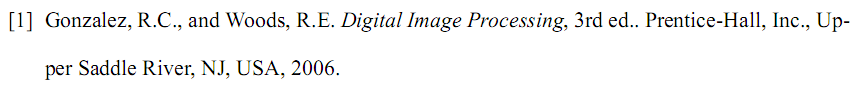
\includegraphics[width=\textwidth]{gonzalez.png}

این شیوهٔ تعریف مراجع بسیار ابتدایی است و اگر فرمت مراجع، ترتیب یا تعداد آنها را خواسته باشید تغییر دهید، به عنوان مثال ابتدا حرف اول نام نویسنده بیاید و سپس نام خانوادگی، باید همه کارها را به صورت دستی انجام دهید!
چون در یک \پ یا مقاله باید کنترل کاملی بر مراجع خود داشته باشید و به راحتی بتوانید قالب مراجع را عوض کنید، بنابراین می‌بایست از \lr{Bib\TeX} استفاده کنید که درپیوست  \ref{app:refMan} به  آن پرداخته خواهد شد.
		% پیوست اول: آشنایی مقدماتی با لاتک
%% !TeX root=../main.tex
%
%\chapter{‌جدول، نمودار و الگوریتم در لاتک}
%\label{app:latex:more}
%%\thispagestyle{empty}
%
%در این بخش نمونه مثالهایی از جدول، شکل، نمودار، الگوریتم و معادلات ریاضی را در لاتک خواهیم دید.
%دقت کنید که در پایان‌نامه‌ها و مقالات، باید قاعدهٔ «ارجاع به جلو%
%\LTRfootnote{Forward Referencing}»
%رعایت شود؛ یعنی ابتدا در متن به شمارهٔ شکل، جدول یا معادله اشاره شود و بعد از آن (زیر آن) خود شکل، جدول یا معادله رسم شود. (توضیحات بیشتر در قسمت
%\ref{sec:floatObjs}).
%
%\section{جدول}
%دستور اصلی برای رسم جدول در لاتک 
%\verb|tabular|
%می‌باشد که جدول
%\eqref{tab:motionModels}
%با استفاده از آن کشیده شده است؛ در
%\verb|tabular|
%عرض جدول برابر با مجموع عرض ستون‌ها و حداکثر مساوی عرض متن است.
%\begin{table}[ht]
%\caption{مدلهای تبدیل.}
%\label{tab:motionModels}
%\centering
%\onehalfspacing
%\begin{tabular}{|r|c|l|r|}
%	\hline نام مدل & درجه آزادی & تبدیل مختصات & توضیح \\ 
%	\hline انتقالی & ۲ & $\begin{aligned} x'=x+t_x \\ y'=y+t_y \end{aligned}$  &  انتقال دوبعدی\\ 
%	\hline اقلیدسی & ۳ & $\begin{aligned} x'=x\cos\theta - y\sin\theta+t_x \\ y'=x\sin\theta+y\cos\theta+t_y \end{aligned}$  &  انتقالی+دوران \\ 
%	\hline 
%\end{tabular} 
%\end{table}
%
%برای اینکه عرض جدول قابل کنترل باشد، باید از دستورات
%\verb|tabularx|،
%\verb|tabulary| یا
%\verb|tabu|
%استفاده کرد که راهنمای آنها در اینترنت وجود دارد.
%مثلاً جدول
%\ref{tab:motionModelsCont}
%با
%\verb|tabularx|
%رسم شده که عرض جدول در آن ثابت بوده و ستون‌های از نوع
%\verb|X|
%عرض خالی جدول را پر می‌کنند.
%\begin{table}[ht]
%	\caption{مدلهای تبدیل دیگر.}
%	\label{tab:motionModelsCont}
%	\centering
%	\onehalfspacing
%	\begin{tabularx}{\textwidth}{|r|c|l|X|}
%		\hline نام مدل & درجه آزادی & تبدیل مختصات & توضیح \\ 
%		\hline مشابهت & ۴ & $\begin{aligned} x'=sx\cos\theta - sy\sin\theta+t_x \\ y'=sx\sin\theta+sy\cos\theta+t_y  \end{aligned}$  & اقلیدسی+تغییرمقیاس \\ 		
%		\hline آفین & ۶ & $\begin{aligned} x'=a_{11}x+a_{12}y+t_x \\ y'=a_{21}x+a_{22}y+t_y \end{aligned}$  & مشابهت+اریب‌شدگی \\
%		\hline
%	\end{tabularx}
%\end{table}
%
%\section{معادلات ریاضی و ماتریس‌ها}
%تقریباً هر آنچه دانشجویان برای نوشتن فرمول‌های ریاضی لازم دارند، در کتاب 
%\lr{mathmode}
%آمده است. کافیست در خط فرمان، دستور زیر را وارد کنید:
%\begin{latin}
%	\texttt{texdoc mathmode}
%\end{latin}
%متن زیر شامل انواعی از اشیاء ریاضی است که با ملاحظه کدش می‌توانید با دستورات آن آشنا شوید.\\
%شناخته‌شده‌ترین روش تخمین ماتریس هوموگرافی الگوریتم تبدیل خطی مستقیم (\lr{DLT\LTRfootnote{Direct Linear Transform}}) است.  فرض کنید چهار زوج نقطهٔ متناظر در دو تصویر در دست هستند،  $\mathbf{x}_i\leftrightarrow\mathbf{x}'_i$   و تبدیل با رابطهٔ
%  $\mathbf{x}'_i = H\mathbf{x}_i$
%  نشان داده می‌شود که در آن:
%\[\mathbf{x}'_i=(x'_i,y'_i,w'_i)^\top  \]
%و
%\[ H=\left[
%\begin{array}{ccc}
%h_1 & h_2 & h_3 \\ 
%h_4 & h_5 & h_6 \\ 
%h_7 & h_8 & h_9
%\end{array} 
%\right]\]
%رابطه زیر را برای الگوریتم  \eqref{alg:DLT} لازم داریم.
%\begin{equation}
%\label{eq:DLT_Ah}
%\left[
%\begin{array}{ccc}
%	0^\top & -w'_i\mathbf{x}_i^\top & y'_i\mathbf{x}_i^\top \\ 
%	w'_i\mathbf{x}_i & 0^\top & -x'_i\mathbf{x}_i^\top \\ 
%	- y'_i\mathbf{x}_i^\top & x'_i\mathbf{x}_i^\top & 0^\top
%\end{array} 
%\right]
%\left(
%\begin{array}{c}
%	\mathbf{h}^1 \\ 
%	\mathbf{h}^2 \\ 
%	\mathbf{h}^3
%\end{array} 
%\right)=0
%\end{equation}
%
%\section{الگوریتم}
%
%\subsection{الگوریتم ساده با دستورهای فارسی}
%با مفروضات فوق، الگوریتم \lr{DLT} به صورت نشان داده شده در الگوریتم \eqref{alg:DLT}  خواهد بود.
%\begin{algorithm}[ht]
%\onehalfspacing
%\caption{الگوریتم \lr{DLT} برای تخمین ماتریس هوموگرافی.} \label{alg:DLT}
%\begin{algorithmic}[1]
%\REQUIRE $n\geq4$ زوج نقطهٔ متناظر در دو تصویر 
%${\mathbf{x}_i\leftrightarrow\mathbf{x}'_i}$،\\
%\ENSURE ماتریس هوموگرافی $H$ به نحوی‌که: 
%$\mathbf{x}'_i = H \mathbf{x}_i$.
%  \STATE برای هر زوج نقطهٔ متناظر
%$\mathbf{x}_i\leftrightarrow\mathbf{x}'_i$ 
%ماتریس $\mathbf{A}_i$ را با استفاده از رابطهٔ \ref{eq:DLT_Ah} محاسبه کنید.
%  \STATE ماتریس‌های ۹ ستونی  $\mathbf{A}_i$ را در قالب یک ماتریس $\mathbf{A}$ ۹ ستونی ترکیب کنید. 
%  \STATE تجزیهٔ مقادیر منفرد \lr{(SVD)}  ماتریس $\mathbf{A}$ را بدست آورید. بردار واحد متناظر با کمترین مقدار منفرد جواب $\mathbf{h}$ خواهد بود.
%  \STATE  ماتریس هوموگرافی $H$ با تغییر شکل $\mathbf{h}$ حاصل خواهد شد.
%\end{algorithmic}
%\end{algorithm}
%
%\subsection{الگوریتم پیچیده و تودرتو با دستورهای فارسی}
%الگوریتم \ref{alg:simulation-random}، یک الگوریتم ترکیبی و تودرتو است که با کمک دستورهای بستهٔ \lr{algorithmic} نوشته شده است.
%
%\begin{algorithm}[p]
%    \onehalfspacing
%    \caption{الگوریتم اجرای برنامهٔ شبیه‌سازی}
%    \label{alg:simulation-random}
%    \begin{algorithmic}[1]
%        \REQUIRE زمان $t_{max}$ به عنوان زمان لازم برای انجام شبیه سازی،\\
%        \REQUIRE  گراف شبکه برای شبیه سازی،
%        \ENSURE جدول تغییرات گراف از لحظهٔ ۰ تا t.
%        \FOR {تمام لحظات در بازهٔ ۰ تا $t_{max}$}
%            \FOR {تمام پیوند‌ها}
%                \STATE محاسبهٔ ضریب و نرخ انتقال پیوند
%                \STATE محاسبهٔ کیفیت و نرخ یادگیری
%            \ENDFOR
%            \FOR {تمام گره‌ها}
%                \STATE محاسبهٔ نرخ انتقال گره
%                \STATE محاسبهٔ وضعیت جدید
%            \ENDFOR
%            \IF {تغییرات از مقدار $\delta$ کمتر است}
%                \STATE شکستن حلقه
%                \COMMENT{این شرط برای پایان قبل از رسیدن به محدودیت زمانی است، اگر تغییرات کمتر از $\delta$ باشد}
%            \ELSIF {زمان اجرای برنامه بیش از حد طول کشیده \AND $t>100$}
%                \STATE شکستن حلقه
%            \ENDIF
%        \ENDFOR
%        \PRINT {زمان اجرای برنامه}
%        \RETURN {ماتریس تغییرات زمانی}
%    \end{algorithmic}
%\end{algorithm}
%
%\subsection{الگوریتم با دستورهای لاتین}
%الگوریتم \ref{alg:RANSAC} یک الگوریتم با دستورهای لاتین است.
%
%\begin{algorithm}[ht]
%\onehalfspacing
%\caption{الگوریتم \lr{RANSAC} برای تخمین ماتریس هوموگرافی.} \label{alg:RANSAC}
%\begin{latin}
%\begin{algorithmic}[1]
%\REQUIRE $n\geq4$ putative correspondences, number of estimations, $N$, distance threshold $T_{dist}$.\\
%\ENSURE Set of inliers and Homography matrix $H$.
%\FOR{$k = 1$ to $N$}
%  \STATE Randomly choose 4 correspondence,
%  \STATE Check whether these points are colinear, if so, redo the above step
%  \STATE Compute the homography $H_{curr}$ by DLT algorithm from the 4 points pairs,
%  \STATE $\ldots$ % الگوریتم کامل نیست
%  \ENDFOR
%  \STATE Refinement: re-estimate H from all the inliers using the DLT algorithm.
%\end{algorithmic}
%\end{latin}
%\end{algorithm}
%
%\section{کد}
%درج کد به زبان‌های مختلف به سادگی امکان‌پذیر است. برنامه
%\ref{code:matlabEx}
%یک قطعه کد
%\lr{MATLAB}
%را نشان می‌دهد.
%\begin{figure}[ht]
%	\begin{LTR}
%        \singlespacing
%		\lstinputlisting[language=MATLAB, caption={نمونه کد \lr{MATLAB}}, label={code:matlabEx}]{MatlabExample.m}
%        % \doublespacing
%	\end{LTR}
%\end{figure}
%
%\section{تصویر}
%نمونهٔ یک تصویر را در فصل قبل دیدیم. دو تصویر شیر کنار هم را نیز در شکل
%\ref{fig:twoLion}
%مشاهده می‌کنید.
%\begin{figure}[ht]
%\centering 
%\subfloat[شیر ۱]{ \label{fig:twolion:one}
%
\includegraphics[width=0.3\textwidth]{lion}}
%%\hspace{2mm}
%\subfloat[شیر ۲]{ \label{fig:twolion:two}
%
\includegraphics[width=0.3\textwidth]{lion}}%
%\caption{دو شیر}
%\label{fig:twoLion} %% label for entire figure
%\end{figure}
%
%\section{نمودار}
%لاتک بسته‌هایی با قابلیت‌های زیاد برای رسم انواع مختلف نمودارها دارد. مانند بسته‌های \lr{Tikz} و  \lr{PSTricks}. توضیح اینها فراتر از این پیوست کوچک است.%
%\footnote{
%مثال‌هایی از بکارگیری بسته
%\lr{Tikz}
%را می‌توانید در
%\url{http://www.texample.net/tikz/examples/}
%ببینید. توصیه می‌شود دانشجویانی که قصد درج اشکالی مانند گراف را در سند خود دارند، مثالهایی از سایت مذکور را ملاحظه فرمایند.
%}
%یک نمودار رسم شده با بستهٔ 
%\lr{TikZ}
% در شکل 
%\ref{fig:parabola}
%نشان داده شده است.
%\begin{figure}[t]
%\centering
%\begin{tikzpicture}[scale=2.5]
%  \shade[top color=blue,bottom color=gray!50] 
%      (0,0) parabola (1.5,2.25) |- (0,0);
%  \draw (1.05cm,2pt) node[above] 
%      {$\displaystyle\int_0^{3/2} \!\!x^2\mathrm{d}x$};
%
%  \draw[style=help lines] (0,0) grid (3.9,3.9)
%       [step=0.25cm]      (1,2) grid +(1,1);
%
%  \draw[->] (-0.2,0) -- (4,0) node[right] {$x$};
%  \draw[->] (0,-0.2) -- (0,4) node[above] {$f(x)$};
%
%  \foreach \x/\xtext in {1/1, 1.5/1\frac{1}{2}, 2/2, 3/3}
%    \draw[shift={(\x,0)}] (0pt,2pt) -- (0pt,-2pt) node[below] {$\xtext$};
%
%  \foreach \y/\ytext in {1/1, 2/2, 2.25/2\frac{1}{4}, 3/3}
%    \draw[shift={(0,\y)}] (2pt,0pt) -- (-2pt,0pt) node[left] {$\ytext$};
%
%  \draw (-.5,.25) parabola bend (0,0) (2,4) node[below right] {$x^2$};
%\end{tikzpicture}
%\caption{یک نمودار زیبا با ارقام فارسی و قابلیت بزرگ‌نمایی بسیار، بدون از دست دادن کیفیت.}
%\label{fig:parabola}
%\end{figure}
%
%\section{نحوه قرارگیری اشیای شناور}
%\label{sec:floatObjs}
%شکل‌ها، جداول و الگوریتم‌ها در لاتک اشیای شناور محسوب می‌شوند؛ یعنی خود لاتک تصمیم می‌گیرد آنها را در کجای صفحه ترسیم کند تا زیباتر باشد. اما می‌توان به لاتک توصیه کرد که آن را در قسمت خاصی از صفحه رسم کند. برای اینکه قاعدهٔ «ارجاع به جلو» رعایت شود باید فقط از پرچم
%\verb|[ht]|
%استفاده کرد، که می‌گوید اگر جا شد شکل را دقیقاً در همین مکان و در غیراینصورت در بالای صفحه بعد رسم کن.
%بنابراین دستورات درج تصویر، جدول و الگوریتم به صورت زیر باید باشند:
%
%\begin{latin}
%\begin{verbatim}
%	\begin{figure/table/algorithm}[ht]
%		...
%	\end{figure/table/algorithm}
%\end{verbatim}
%\end{latin}
		% پیوست دوم: جدول، نمودار و الگوریتم در لاتک
%% !TeX root=../main.tex
%\chapter{مراجع، واژه‌نامه و حاشیه‌نویسی}
%\label{app:refMan}
%%\thispagestyle{empty}
%
%\section{مراجع و نقل‌قول‌ها}
%\label{sec:refUsage}
%منابعِ پایان‌نامه، پایه و اساس تحقیق شما به حساب می‌آیند و ضرورت انجام مطالعه و روش‌های به کار رفته در بسیاری از قسمت‌های آن، به کمک منابع صورت می‌گیرد. در استفاده از مراجع علمی در پایان‌نامه، باید سعی کنید بیشتر از
%\textbf{منابع چاپ‌شده و مهم}
%استفاده کنید و
%\emph{ارجاع به داده‌های چاپ نشده، خلاصه‌ها و پایان‌نامه‌ها، سبب به‌هم‌خوردگی و کاهش اعتبار قسمت ارجاع منابع می‌شود.}
%استفاده از منابع و نقل قول‌هایی به تحقیق شما ارزش می‌دهند که
%\textbf{در راستای هدف تحقیق بوده و به آن اعتبار ببخشند.}
%برخی از دانش‌جویان تصوّر می‌کنند که کثرت نقل‌قول‌ها و ارجاعات زیاد، مهم‌ترین معیار علمی شدن پایان‌نامه است؛ حال آنکه استناد به تعداد کثیری از منابع بدون مطالعه دقیق آنها و استفادهٔ مستقیم در پایان‌نامه، می‌تواند نشان‌دهندهٔ عدم احساس امنیت نویسنده باشد!
%
%دو روش برای استفاده از نتایج، جملات، داده‌ها و روش‌های دیگران وجود دارد. یکی نقل‌قول مستقیم و دقیق است و دیگری استفاده غیرمستقیم در متن مقاله، که در ادامه به قواعد این دو نوع نقل‌قول و ارجاع‌دهی اشاره می‌کنیم:
%\begin{description}
%	\item[نقل‌قول مستقیم:]
%	نقل‌قول مستقیم باید دقیق و بدون هیچ تغییری در جملات باشد. بهتر است این‌گونه نقل‌قول‌ها تا حد امکان کوتاه باشد. جملات کوتاه داخل گیومه قرار می‌گیرند و باید به منبع دقیق آن، طبق روش ارجاع‌دهی به منابع، اشاره شود. به عنوان مثال در
%	\cite{persianbib87userguide}
%	آمده است که:
%	\begin{quote}
%		«با استفاده از فیلد
%		\lr{AUTHORFA}
%		می‌توان معادل فارسی نام نویسندگان مقالات لاتین را در متن داشت. معمولاً در اسناد فارسی خواسته می‌شود که پس از ذکر معادل فارسی نام نویسنده، نام لاتین نویسنده(ها) به عنوان پاورقی درج شود
%		\citep{persianbib87userguide}.»
%	\end{quote}
%	\item[نقل‌قول غیرمستقیم:]
%	نقل‌قول غیرمستقیم به معنی استفاده از ایده‌ها، نتایج، روش‌ها و داده‌های دیگران در درون متنِ پایان‌نامه، ولی به سبک خودتان و متناسب و هماهنگ با روند پایان‌نامهٔ شماست. در این حالت نیز باید متناسب با شیوهٔ ارجاع‌دهی به آن استناد شود.
%\end{description}
%
%با توجه به وجود سبک‌های مختلف ارجاع‌دهی، باید
%\textbf{روش قابل قبول و یکسانی}
%در طول پایان‌نامه برای اشاره به مراجع در متن و همچنین تهیه فهرست مراجع در انتهای پایان‌نامه بکار رود. مثلاً برای پایان‌نامه‌های مهندسی می‌توان از سبک ارجاع‌دهی
%\lr{IEEE}%
%\LTRfootnote{\url{http://www.ieee.org/documents/ieeecitationref.pdf}}
%یا
%\lr{acm}
%استفاده کرد. طبیعتاً باید تناظر یک‌به‌یک بین فهرست مراجع در انتهای گزارش و مراجع مورد استفاده در متن باشد%
%\footnote{البته گاهی ممکن است محقق مرجعی را مورد مطالعه قرار داده لیکن در متن به آن اشاره نکرده باشد؛ برخی معتقدند در این موارد نیز آوردن آن در فهرست مراجع، اشکالی ندارد، به این شرط که از عنوان «فهرست منابع» به جای «فهرست مراجع» استفاده شود.}.
%
%برای سهولت مدیریت مراجعِ \پ%
%، اکیداً توصیه می‌شود از یک ابزار «مدیریت منابع» (با خروجی
%\texorpdfstring{\lr{Bib\TeX}}{Bib\TeX}%
%) همچون
%\lr{Mendeley}،
%\lr{Zotero},
%\lr{EndNote}
%یا
%\lr{Citavi}
%استفاده کنید.
%
%\subsection{ مدیریت مراجع با  \texorpdfstring{\lr{Bib\TeX}}{Bib\TeX}}
%در بخش \ref{Sec:Ref} اشاره شد که با دستور 
% \lr{\textbackslash bibitem}
%  می‌توان یک مرجع را تعریف نمود و با فرمان
% \lr{\textbackslash cite}
%  به آن ارجاع داد. این روش برای تعداد مراجع زیاد و تغییرات آنها مناسب نیست. برای مدیریت منابع زیاد، سه بستهٔ
%\lr{BibTeX} (پیش‌فرض),
%\lr{natbib}
%(ارجاع‌دهی در متن به صورت نویسنده-سال)
%و \lr{BibLaTeX} (جدید و منعطف‌پذیر)
%وجود دارند. در ادامه توضیحاتی در مورد مدیریت منابع با \lr{BibTeX} و \lr{natbib} در زی‌پرشین خواهیم آورد که همراه با توزیع‌های معروف تِک عرضه می‌شوند
%\footnote{روش \lr{BibLaTeX} هنوز برای متون فارسی به درستی ترجمه نشده است.}.
%
%یکی از روش‌های قدرتمند و انعطاف‌پذیر برای نوشتن مراجعِ مقالات و مدیریت مراجع در لاتک، استفاده از  \lr{BibTeX} است.
% روش کار با بیب‌تک به این صورت است که مجموعهٔ همهٔ مراجعی را که در \پ استفاده کرده یا خواهیم کرد، 
%در پروندهٔ جداگانه‌ای با پسوند
%\lr{bib}
%نوشته و به آن فایل در سند خودمان به صورت مناسب لینک می‌دهیم.
% کنفرانس‌ها یا مجله‌های گوناگون برای نوشتن مراجع، قالب‌ها یا قراردادهای متفاوتی دارند که به آنها استیل‌های مراجع گفته می‌شود.
% در این حالت به کمک ‌استیل‌های بیب‌تک خواهید توانست تنها با تغییر یک پارامتر در پروندهٔ ورودی خود، مراجع را مطابق قالب موردنظر تنظیم کنید. 
% بیشتر مجلات و کنفرانس‌های معتبر یک فایل سبک
% (\lr{BibTeX Style})
%با پسوند \lr{bst} در وب‌گاه خود می‌گذارند که برای همین منظور طراحی شده است.
%
%به جز نوشتن مقالات، این سبک‌ها کمک بسیار خوبی برای تهیهٔ مستندات علمی همچون پایان‌نامه‌هاست که فرد می‌تواند هر قسمت از کارش را که نوشت مراجع مربوطه را به بانک مراجع خود اضافه نماید. با داشتن چنین بانکی از مراجع، وی خواهد توانست به راحتی یک یا چند ارجاع به مراجع و یا یک یا چند بخش را حذف یا اضافه ‌نماید؛ 
%مراجع به صورت خودکار مرتب شده و
%\textbf{فقط مراجع ارجاع داده شده در قسمت کتاب‌نامه خواهندآمد.}
%قالب مراجع به صورت یکدست مطابق سبک داده شده بوده و نیازی نیست که کاربر درگیر قالب‌دهی به مراجع باشد. 
%
%\subsection{سبک‌های مورد تأیید دانشگاه تهران}
%طبق «دستورالعمل نگارش و تدوین پایان‌نامه» دانشگاه تهران در
%\cite{UTThesisGuide}،
%ارجاع در متن می‌تواند مطابق با هر یک از دو الگوی هاروارد یا ونکوور باشد:
%\singlespacing
%\begin{description}
%	\item[سیستم نویسنده-سال (هاروارد):]
%	ذکر نام نویسنده و سال نشر در متن. در این الگو مراجع بر اساس حروف الفبا تنظیم می‌گردند.
%	\item[سیستم شماره‌دار (ونکوور):]
%	ارجاع به مراجع به کمک شماره در متن. در این الگو شماره هر مرجع به ترتیب ظاهر شدن آن در متن در داخل کروشه قرار می‌گیرد. فهرست مراجع نیز بر اساس شماره مرجع (نه حروف الفبا) تنظیم می‌گردد.
%\end{description}
%\doublespacing
%
%در مدیریت منابع با
%\lr{\textbf{BibTeX}}،
%ارجاع‌ها در متن تنها به شکل
%\textbf{شماره‌دار (ونکوور)}
%امکان‌پذیر است، گرچه فهرست مراجع می‌تواند با روش‌های مختلف مرتب شود. اگر بخواهیم ارجاع‌ها در متن به صورت
%\textbf{نویسنده-سال (هاروارد)}
%باشد باید از بستهٔ
%\lr{\textbf{natbib}}\LTRfootnote{Natural Sciences Citations \& References}
%و استیل‌های مختلف آن استفاده کنیم.
%
%هنگام استفاده از روش نویسنده-سال نوع پرانتزگذاری‌ها در وسط و انتهای جمله با هم فرق خواهد داشت. به مثال زیر مطابق با دستورالعمل
%\cite{UTThesisGuide}
%توجه کنید:
%
%\textit{
%ابتدا
%\cite{Khalighi87xepersian}
%بستهٔ زی‌پرشین را برای حروف‌چینی فارسی اختراع کرد. بعدها سبک‌های ارجاع‌دهی فارسی و قالب‌های پایان‌نامه نیز مبتنی بر آن ساخته شد
%\citep{persianbib87userguide}.
%ارجاع‌دهی به مراجع لاتین نیز در زی‌پرشین امکان‌پذیر است. مثلاً
%\citelatin{Gonzalez02book}
%یک کتاب انگلیسی است و به راحتی به مقالات انگلیسی نیز می‌توان ارجاع داد
%\citeplatin{kim2016integrated}.}
%
%در این مثال، ۴ ارجاع در وسط و انتهای جمله به مراجع فارسی و انگلیسی آمده است. وقتی از سیستم نویسنده-سال استفاده می‌کنید، بهتر است ارجاع‌های آخر جمله کلاً داخل پرانتر بیاید؛ بدین منظور باید به جای
%\verb|\cite|
%از
%\verb|\citep|
%استفاده کنید. اما در سیستم شماره‌دار چون تمام ارجاع‌ها داخل کروشه می‌آیند این امر اهمیت ندارد.\\
%نمی‌توانید در متن فارسی، اسم لاتین محقق خارجی را بیاورید و برای جلوگیری از ایجاد ابهام، صرف‌نظر از نام لاتین هم مجاز نیست! توصیه می‌شود که نام محقق خارجی در متن با حروف فارسی و در پاورقی اسم تمام نویسندگان به صورت انگلیسی آورده شود. نحوهٔ رعایت این نکته را می‌توانید در کد مثال بالا ببینید.
%
%گرچه در تمپلت ورد
%\cite{UTThesisGuide}،
%به صراحت ذکر شده که بهتر است برای پایان‌نامه‌های مهندسی از سبک 
%\lr{IEEE}
%استفاده شود (که از سیستم ونکوور تبعیت می‌کند)، اما ترتیب فهرست مراجع در
%\lr{IEEE}
%بر اساس ترتیب ارجاع در متن بوده و
%\emph{مراجع انگلیسی و فارسی از هم تفکیک نمی‌شوند}
%که متضاد با دستورالعمل
%\cite{UTThesisGuide}
%و نیز متضاد عرف اکثر پایان‌نامه‌های فارسی است.
%بنابراین دقیقاً نمی‌توان سبک خاصی را برای مراجع پایان‌نامه‌های دانشگاه تهران اجبار کرد. مهم این است که
%\textbf{سبک ارجاع‌دهی در تمام طول یک کتابچه}
%(مثلاً پایان‌نامه، مقالات یک مجله یا کل یک کتاب) یکسان باشد. بهتر است
%\textbf{بسته به حوزه پایان‌نامه}،
%در این مورد با استاد راهنمای خود مشورت کنید.
%
%\subsection{سبک‌های فارسی قابل استفاده در زی‌پرشین}
%تعدادی از سبک‌های فارسی بسته
%\lr{Persian-bib}%
%\footnote{ برای اطلاع بیشتر به راهنمای بستهٔ
%\lr{Persian-bib}
%مراجعه فرمایید.}
%که برای  زی‌پرشین آماده شده‌اند، عبارتند از:
%
%\singlespacing
%\begin{itemize}
%\item \emph{سبک‌های شماره‌دار}:
%	\begin{description}
%	\item [unsrt-fa.bst] این سبک متناظر با \lr{unsrt.bst} می‌باشد. مراجع به ترتیب ارجاع در متن ظاهر می‌شوند.
%	\item [plain-fa.bst] این سبک متناظر با \lr{plain.bst} می‌باشد. مراجع بر اساس نام‌خانوادگی نویسندگان، به ترتیب صعودی مرتب می‌شوند.
%	 همچنین ابتدا مراجع فارسی و سپس مراجع انگلیسی خواهند آمد.
%	\item [acm-fa.bst] این سبک متناظر با \lr{acm.bst} می‌باشد. شبیه \lr{plain-fa.bst} است.  قالب مراجع کمی متفاوت است. اسامی نویسندگان انگلیسی با حروف بزرگ انگلیسی نمایش داده می‌شوند. (مراجع مرتب می‌شوند)
%	\item [ieeetr-fa.bst] این سبک متناظر با \lr{ieeetr.bst} می‌باشد. (مراجع مرتب نمی‌شوند)
%	\end{description}
%	
%\item \emph{سبک‌های نویسنده-سال}:
%	\begin{description}
%	\item [plainnat-fa.bst] این سبک متناظر با \lr{plainnat.bst} می‌باشد. نیاز به بستهٔ \lr{natbib} دارد. (مراجع مرتب می‌شوند)
%	\item [chicago-fa.bst] این سبک متناظر با \lr{chicago.bst} می‌باشد. نیاز به بستهٔ \lr{natbib} دارد. (مراجع مرتب می‌شوند)
%	\item [asa-fa.bst] این سبک متناظر با \lr{asa.bst} می‌باشد. نیاز به بستهٔ \lr{natbib} دارد. (مراجع مرتب می‌شوند)
%	\end{description}
%\end{itemize}
%\doublespacing
%
%با استفاده از استیل‌های فوق می‌توانید به انواع مختلفی از مراجع فارسی و لاتین ارجاع دهید.
%به عنوان مثال‌هایی از
%\textbf{مراجع انگلیسی}،
%مرجع
%\cite{Baker02limits}\footnote{چون فیلد \lr{authorfa} برای این مرجع تعریف نشده در سبک نویسنده-سال با حروف لاتین به آن در متن ارجاع می‌شود که غلط است.}
%مقالهٔ یک ژورنال، مرجع
%\cite{Amintoosi09video}
%مقالهٔ یک کنفرانس، مرجع
%\citelatin{Gonzalez02book}
%یک کتاب، مرجع
%\cite{Khalighi07MscThesis}
%پایان‌نامهٔ کارشناسی ارشد و مرجع
%\citelatin{Borman04thesis}
%یک رسالهٔ دکتری می‌باشد.\\
%همچنین در میان
%\textbf{مراجع فارسی},
%مرجع
%\cite{Vahedi87}
%مقالهٔ یک مجله، مرجع
%\cite{Amintoosi87afzayesh}
%مقالهٔ یک کنفرانس، مرجع
%\cite{Pedram80osool}
%یک کتاب ترجمه‌شده با ذکر مترجمان و ویراستاران، مرجع
%\cite{Pourmousa88mscThesis}
%پایان‌نامهٔ کارشناسی ارشد%
%\footnote{همان‌طور که در بخش
%\ref{sec:refUsage}
%اشاره شد، بهتر است زیاد از پایان‌نامه‌ها در مراجع استفاده نکنید.}،
%مرجع
%\cite{Omidali82phdThesis}
%یک رسالهٔ دکتری و مراجع
%\cite{persianbib87userguide, Khalighi87xepersian}
%نمونه‌های متفرقه هستند.
%
%\subsection{ساختار فایل مراجع}
%برای استفاده از بیب‌تک باید مراجع خود را در یک فایل با پسوند \lr{bib} ذخیره نمایید. یک فایل \lr{bib} در واقع یک پایگاه داده از مراجع%
%\LTRfootnote{Bibliography Database}
%شماست که هر مرجع در آن به عنوان یک رکورد از این پایگاه داده
%با قالبی خاص ذخیره می‌شود. به هر رکورد یک مدخل%
%\LTRfootnote{Entry}
%گفته می‌شود. یک نمونه مدخل برای معرفی کتاب \lr{Digital Image Processing} در ادامه آمده است:
%
%\singlespacing
%\begin{LTR}
%\begin{verbatim}
%@BOOK{Gonzalez02image,
%  AUTHOR     = {Gonzalez,, Rafael C. and Woods,, Richard E.},
%  TITLE      = {Digital Image Processing},
%  PUBLISHER  = {Prentice-Hall, Inc.},
%  YEAR       = {2006},
%  ISBN       = {013168728X},
%  EDITION    = {3rd},
%  ADDRESS    = {Upper Saddle River, NJ, USA}
%}
%\end{verbatim}
%\end{LTR}
%\doublespacing
%
%در مثال فوق، \lr{@BOOK} مشخصهٔ شروع یک مدخل مربوط به یک کتاب و \lr{Gonzalez02book} برچسبی است که به این مرجع منتسب شده است.
% این برچسب بایستی یکتا باشد. برای آنکه بتوان
%\textbf{برچسب مراجع}
% را به راحتی به خاطر سپرد و حتی‌الامکان برچسب‌ها متفاوت با هم باشند، معمولاً از قوانین خاصی به این منظور استفاده می‌شود. یک قانون می‌تواند
%\textbf{فامیل نویسنده اول + دورقم سال نشر + اولین کلمهٔ عنوان اثر}
%باشد. به
%\lr{AUTHOR}، \lr{TITLE}، $\dots$ و \lr{ADDRESS}
%فیلدهای این مدخل گفته می‌شود، که هر یک با مقادیر مربوط به مرجع پر شده‌اند. ترتیب فیلدها مهم نیست. 
%
%انواع متنوعی از مدخل‌ها برای اقسام مختلف مراجع همچون کتاب، مقالهٔ کنفرانس و مقالهٔ ژورنال وجود دارد که برخی فیلدهای آنها با هم متفاوت است. 
%نام فیلدها بیانگر نوع اطلاعات آن می‌باشد. مثالهای ذکر شده در فایل \lr{MyReferences.bib} کمک خوبی برای شما خواهد بود. 
%%این فایل یک فایل متنی بوده و با ویرایشگرهای معمول همچون \lr{Notepad++} قابل ویرایش می‌باشد. برنامه‌هایی همچون 
%%\lr{TeXMaker}
%% امکاناتی برای نوشتن این مدخل‌ها دارند و به صورت خودکار فیلدهای مربوطه را در فایل \lr{bib}  شما قرار می‌دهند.  
%با استفاده از سبک‌های فارسی آماده شده، محتویات هر فیلد می‌تواند به فارسی نوشته شود؛ ترتیب مراجع و نحوهٔ چینش فیلدهای هر مرجع را سبک مورد استفاده  مشخص خواهد کرد.
%
%\textbf{در فایل 
%\lr{MyReferences.bib}
% که همراه با این \پ هست، مثال‌های مختلفی از مراجع آمده‌اند که برای درج مراجع خود، تنها کافیست مراجع‌تان را جایگزین موارد مندرج در آن نمایید.
%}
%
%برای بسیاری از مقالات لاتین حتی لازم نیست که مدخل مربوط به آنرا خودتان بنویسید. با جستجوی 
%\textbf{نام مقاله + کلمه
%\lr{bibtex}}
%در اینترنت سایت‌های بسیاری همچون
%\lr{ACM} و \lr{ScienceDirect}
%را خواهید یافت که مدخل
%\lr{bibtex}
%مربوط به مقاله شما را دارند و کافیست آنرا به انتهای فایل
%\lr{MyReferences.bib}
%اضافه کنید.
%
%\subsection{نحوه اجرای \texorpdfstring{\lr{Bib\TeX}}{Bib\TeX}}
%پس از قرار دادن مراجع خود، برای ساخت فایل خروجی می‌توانید دستور زیر را (در ترمینال یا از طریق \lr{Texmaker}) اجرا کنید:%
%\footnote{فایل \lr{latexmkrc} باید در کنار \lr{main.tex} وجود داشته باشد.}
%
%\singlespacing
%\begin{LTR}
%	\begin{verbatim}
%		latexmk -bibtex -pdf main.tex
%	\end{verbatim}
%\end{LTR}
%\doublespacing
%ابزار \lr{latexmk} مراحل مختلف ساخت خروجی لاتک را به طور خودکار و بهینه انجام می‌دهد و هر بار فقط مراحلی را که لازم باشد تکرار می‌کند.
%روش دستی‌تر این است که یک بار \lr{XeLaTeX} را روی سند خود اجرا نمایید، سپس \lr{bibtex} و پس از آن هم ۲ بار \lr{XeLaTeX} را. در \lr{TeXMaker} کلید \lr{F11} و در \lr{TeXWorks} هم گزینهٔ \lr{BibTeX} از منوی \lr{Typeset}، \lr{BibTeX} را روی سند شما اجرا می‌کنند.
%
%\section{واژه‌نامه‌ها و فهرست اختصارات}
%\gls{Gloss}
%یا فرهنگ لغات، مجموعه‌ای از اصطلاحات و تعاریف خاص و فنی است که معمولاً در انتهای یک کتاب می‌آید. چون پایان‌نامه خود یک متن تخصصی بلند محسوب می‌شود، استفاده از فرهنگ لغات در انتهای آن به شدت توصیه می‌شود، خصوصاً که احتمال استفاده از لغات تخصصی لاتین در آن بالاست.
%واژه‌نامه‌هایی که در انتهای کتاب‌های انگلیسی می‌آیند معمولاً تک‌زبانه هستند و معنی یک اصطلاح تخصصی در آنها، عمدتاً به صورت یک
%\gls{Description}
%طولانی آورده می‌شود. اما چون در متون فارسی، آوردن لغات انگلیسی مجاز نیست و باید معادل فارسی آنها وارد شود، جهت رفع ابهام معمولاً واژه‌نامهٔ فارسی به انگلیسی (و برعکس) در انتهای کتاب درج شده و  
%\glspl{Description}
%در صورت نیاز در متن آورده می‌شوند.
%
%فهرست
%\glspl{Acronym}
%شامل نمادهای کوتاهی است که اغلب از حروف ابتدایی کلمات یک عبارت طولانی ساخته شده‌اند. با اینکه
%\glspl{Acronym}
%با حروف (بزرگ) لاتین نوشته می‌شوند، اما چون کوتاهند استفاده از آنها در میان متن فارسی مجاز است. با این حال برای رفع ابهام، عرف است که فهرستی از آنها شامل معنی هر نماد، در کنار دیگر فهرست‌ها در ابتدای متن درج شود.
%
%در این قالب پایان‌نامه، برای ساخت و مدیریت واژه‌نامه و فهرست اختصارات از بستهٔ پیشرفتهٔ
%\lr{glossaries}
%با موتور واژه‌نامه‌سازی
%\lr{xindy}
%استفاده می‌شود. تنظیمات بهینهٔ این بسته در فایل
%\lr{glossaries-settings.tex}
%عبارتند از:
%\begin{itemize}
%	\item
%قبل از درج واژه‌ها در متن، باید مدخل آنها با دستور زیر (ترجیحاً در فایل جدای \lr{words.tex}) تعریف شود:
%	\begin{LTR}
%	\verb|\newword{Label}{Word}|\{واژه\}\{واژه‌ها\}
%	\end{LTR}
%	
%	\item
%قبل از وارد کردن علائم اختصاری در متن، باید مدخل آنها نیز (ترجیحاً در فایل \lr{acronyms.tex}) به صورت زیر تعریف شود:
%	\begin{LTR}
%	\verb|\newacronym{Label}{Acr}|\{معنی‌اختصار\}
%	\end{LTR}
%
%	\item
%جهت درج یک علامت اختصاری یا معادل یک واژه تخصصی، کافی است از دستور
%	\verb|gls{Label}|
%در متن استفاده کنید. دستور
%	\verb|glspl{Label}|
%نیز برای آوردن معادل یک لغت در حالت جمع ساخته شده است.
%	
%	\item
%هنگام اولین استفاده از یک معادل فارسی یا اختصار در متن، معادل انگلیسی یا معنی آن در پاورقی آورده می‌شود. در صورتی که هر یک از این پیش‌فرض‌ها را دوست ندارید با ویرایش فایل
%	\lr{glossaries-settings.tex}
%می‌توانید آن را تغییر دهید.
%
%	\item
%در انتهای پایان‌نامه با دستور
%\verb|\printglossary|
%فهرست کلمات استفاده‌شده به ترتیب الفبای فارسی (واژه‌نامه فارسی به انگلیسی) و الفبای انگلیسی (واژه‌نامه انگلیسی به فارسی) درج می‌شود.
%\end{itemize}
%
%به عنوان مثال، با مشاهدهٔ کد این نوشته، نحوهٔ درج معادل فارسی
%\gls{RandomVariable}
%را در متن مشاهده می‌کنید.
%در نمایش واژهٔ
%\gls{RandomVariable}
%برای بار دوم، معادل لاتین در پاورقی نمی‌آید.
%در مورد درج علائم اختصاری، مثلاً می‌توان به رابطهٔ
%\gls{F}
%اشاره کرد.
%
%\section{حاشیه‌نویسی در نسخه پیش‌نویس}
%اصلاح و بازبینی چندین و چندبارهٔ یک پایان‌نامه یا مقاله، از معمول‌ترین امور در نگارش آن می‌باشد. فرض کنید دانشجو پایان‌نامه یا مقالهٔ خود را (کامل یا ناقص) نوشته و می‌خواهد نظر استاد راهنما، اعضای آزمایشگاه یا دیگر متخصصین را در مورد آن جویا شود. به جز مشاورهٔ حضوری، تلفنی یا از طریق ایمیل، برای اظهارنظر دقیق بر نوشته، می‌توان از ابزارهای حاشیه‌نویسی در فایل
%\lr{PDF}
%یا \lr{tex}
%نیز استفاده کرد.
%
%یک راهکار مناسب برای حاشیه‌نویسی در فایل \lr{tex}، استفاده از بسته 
%\lr{todonotes}
%می‌باشد که آقای خلیقی به تازگی امکان استفاده از آن را برای فارسی‌زبانان نیز فراهم آورده‌اند.
%بدین منظور، هر جایی که خواستید نکته یا نکاتی را در حاشیه متن یادداشت کنید، کافی است دستور زیر را وارد نمایید:
%\begin{latin}
%\verb|\todo{NOTE}|
%\end{latin}
%مثلاً استاد راهنما می‌تواند از دانشجو بخواهد که در بخشی توضیح بیشتری دهد.
%\todo{
%توضیح بیشتری لازم است.
%}
%استاد راهنما یا داور حتی می‌تواند محل پیشنهادی برای درج یک تصویر را نیز به راحتی برای دانشجو مشخص کند.
%\missingfigure[figwidth=\textwidth,figcolor=white]{یک تصویر از خروجی الگوریتم 
%\ref{alg:RANSAC}
%را در اینجا قرار دهید.}
%یکی دیگر از امکانات این بسته آن است که می‌توان فهرست نکات را در ابتدای سند داشت. بسته 
%\lr{todonotes}
%امکانات بسیاری دارد
%\todo[fancyline,color=green!30]{مرجع این مطلب؟}
%که در راهنمای آن معرفی شده است و با اجرای دستور زیر در خط فرمان می‌توانید آنها را مشاهده کنید:
%\begin{latin}	
%	\texttt{texdoc todonotes}
%\end{latin}	
%دقت کنید که توضیحات حاشیه‌ای و فهرست کارهای باقیمانده (نکات)،
%\textbf{فقط در نسخه
%\gls{Draft}}
%قابل دیدن هستند و در نسخه نهایی، نمایش داده نخواهند شد.
%برای استفاده از حالت
%\gls{Draft}
%باید گزینه 
%\lr{draft}
%به دستور 
%\verb|\documentclass|
%در ابتدای فایل 
%\lr{main.tex}
%اضافه شود.
%هنگامی‌که سند شما در حالت 
%\gls{Draft}
%باشد:
%
%\singlespacing
%\begin{enumerate}
%\item 
%هیچ یک از صفحات آغازین پایان‌نامه، تا فهرست مطالب نمایش داده نمی‌شود (به جز صفحه اول).
%\item
%روی صفحه اول عبارت «پیش‌نویس» به صورت درشت و کم‌رنگ نمایش داده می‌شود.
%\item
%فهرست نکات درج شده توسط
%\lr{todo}،
%پس از فهرست اصلی و با عنوان «فهرست کارهای باقیمانده» نمایش داده می‌شود.
%\item
%شماره صفحاتی که به هر مرجع ارجاع داده شده است در بخش مراجع نمایش داده می‌شود
%\footnote{اعمال گزینهٔ
%\lr{pagebackref}
%برای بستهٔ
%\lr{hyperref}.
%}.
%\end{enumerate}
%\doublespacing
%هر یک از موارد بالا تا زمانی که نسخه نهایی \پ نیاز نباشد بسیار مورد توجه و مفید واقع می‌شوند.
   	% پیوست سوم: مراجع، واژه‌نامه و حاشیه‌نویسی

% برگرداندن شماره‌بندی صفحات فصول
% \let\chapter\Chapter
\pagenumbering{tartibi} % اول، دوم، ...
%\baselineskip=.75cm

% چاپ واژه‌نامه‌ها و نمایه 
\onehalfspacing
\cleardoublepage
\printglossary
\cleardoublepage
\printindex

\begin{latin}
\baselineskip=.6cm
\latinabstract
\latinTitlePage
\end{latin}
\label{LastPage}

\end{document}
